
\documentclass[usenames,dvipsnames,aspectratio=169,11pt,handout]{beamer}
%handout,
%aspectratio=43

\usepackage{Others/prespreamble}
\usepackage{natbib}
\usepackage[normalem]{ulem}
\usepackage{colortbl, xcolor}
\definecolor{RoyalBlue}{rgb}{0.19, 0.55, 0.91}
\linespread{1}
\usepackage{mathrsfs}

% small bibliography
\let\oldthebibliography=\thebibliography
\renewcommand{\thebibliography}[1]{
    \oldthebibliography{#1}
    \setlength{\itemsep}{2pt}
    \tiny
}

\begin{document}

\begin{frame}[noframenumbering,plain]
	\maketitle
	%\begin{figure}[H]
	%\centering
	%\includegraphics[scale=0.4]{Other/Figures/erc.png}
	%\end{figure}

	%\footnotesize{Funding from the European Research Council (ERC) under the European Unions Horizon 2020 research and innovation programme (grant agreement No. 789111 - ERC EvolvingEconomics) is gratefully acknowledged}
\end{frame}
%\frame{\titlepage}

\begin{frame}\frametitle{Motivation}

	Individuals \textbf{distort} or \textbf{avoid} new information:

	\vfill

	\begin{wideitemize}
		\item investors overreact to good news \citep{danielOverconfidentInvestorsPredictable2015};
		\item charity donors ignore the impact of their donation \citep{niehausTheoryGoodIntentions2014};
		\item medical patients avoid testing \citep{golmanInformationAvoidance2017}.
	\end{wideitemize} \pause

	\vfill

	A possible rationalisation is that individuals care about beliefs \textit{per se}:

	\vfill

	\begin{wideitemize}
		\item well-being depends on beliefs;
		\item belief revision depends on preferences;
		\item hard to identify beliefs, preferences and updating rule.
	\end{wideitemize}

\end{frame}

\begin{frame}\frametitle{This paper}
	This paper:

	\vfill

	\begin{wideenumerate}
		\item Dynamic model of belief-dependent preferences (BDP);
		\item Axiomatic characterisation of such a model;
		\item Derivation of individuals' belief updating rule, which depends on preferences.
	\end{wideenumerate} \pause

	\vfill

	Main contribution:
	\vfill
	\begin{wideitemize}
		\item testable predictions;
		\item joint identification of beliefs, preferences and updating rule.
	\end{wideitemize}

\end{frame}

\begin{frame}\frametitle{Model in a nutshell}

	Key features:

	\vfill

	\begin{wideitemize}
		\item the individual cares about beliefs per se;
		\item she \textbf{distorts beliefs} away from Bayesian updating to increase her welfare;
		\item she is then \textbf{tempted} to act according to her distorted beliefs;
		\item ex ante, she \textbf{anticipates} such belief and choice distortion. \footnotesize{\citep{cobb-clarkPredictivePowerSelfcontrol2022}}
	\end{wideitemize}

	\vfill \pause

	\textbf{Main result}: axiomatic characterisation of BDP preferences and updating rules.

\end{frame}

\begin{frame}[noframenumbering,plain]\frametitle{Outline}

	\tableofcontents

\end{frame}

\section{Illustration of the model through an example}

\begin{frame}{Illustrative Example}

	An investor chooses whether to check her portfolio or not.

	\vfill

	If she does, she observes prices and can invest or do nothing. \pause

	\vfill

	\begin{table}[H]
		\centering


		\tikzset{every picture/.style={line width=0.75pt}} %set default line width to 0.75pt        

		\begin{tikzpicture}[x=0.75pt,y=0.75pt,yscale=-1,xscale=1]
			%uncomment if require: \path (0,341); %set diagram left start at 0, and has height of 341

			%Straight Lines [id:da6521689763503256] 
			\draw [color=RoyalBlue, draw opacity=1]   (259.33,139.1) -- (366.63,99.41) ;
			%Straight Lines [id:da3094065715046459] 
			\draw [color=Red, draw opacity=1]   (259.33,139.1) -- (366.63,178.91) ;
			%Straight Lines [id:da3636097363244992] 
			\draw [color=RoyalBlue, draw opacity=1]   (259.33,139.1) -- (366.63,139.41) ;
			%Straight Lines [id:da7301255340273027] 
			\draw  [dash pattern={on 0.84pt off 2.51pt}]  (369,99.41) -- (369,139.41) ;
			%Shape: Circle [id:dp5572573680385027] 
			\draw   (366.63,99.41) .. controls (366.63,98.09) and (367.69,97.03) .. (369,97.03) .. controls (370.31,97.03) and (371.38,98.09) .. (371.38,99.41) .. controls (371.38,100.72) and (370.31,101.78) .. (369,101.78) .. controls (367.69,101.78) and (366.63,100.72) .. (366.63,99.41) -- cycle ;
			%Shape: Circle [id:dp045414237311399264] 
			\draw   (366.63,139.41) .. controls (366.63,138.09) and (367.69,137.03) .. (369,137.03) .. controls (370.31,137.03) and (371.38,138.09) .. (371.38,139.41) .. controls (371.38,140.72) and (370.31,141.78) .. (369,141.78) .. controls (367.69,141.78) and (366.63,140.72) .. (366.63,139.41) -- cycle ;
			%Shape: Circle [id:dp6206756734194616] 
			\draw   (366.63,178.91) .. controls (366.63,177.59) and (367.69,176.53) .. (369,176.53) .. controls (370.31,176.53) and (371.38,177.59) .. (371.38,178.91) .. controls (371.38,180.22) and (370.31,181.28) .. (369,181.28) .. controls (367.69,181.28) and (366.63,180.22) .. (366.63,178.91) -- cycle ;

			% Text Node
			\draw (277.54,114.19) node [anchor=north west][inner sep=0.75pt]  [color=RoyalBlue ,opacity=1 ,rotate=-339.07]  {$Good$};
			% Text Node
			\draw (314.98,142.65) node [anchor=north west][inner sep=0.75pt]  [font=\small,color=RoyalBlue ,opacity=1 ]  {$Normal$};
			% Text Node
			\draw (211.83,130.7) node [anchor=north west][inner sep=0.75pt]    {$Check$};
			% Text Node
			\draw (294.77,155.06) node [anchor=north west][inner sep=0.75pt]  [color=Red ,opacity=1 ,rotate=-19.16]  {$Bad$};
			% Text Node
			\draw (371.33,156.4) node [anchor=north west][inner sep=0.75pt]  [color=Red ,opacity=1 ]  {$\overset{\underline{p}}{\{invest, nothing\}}$};
			% Text Node
			\draw (370.83,98.4) node [anchor=north west][inner sep=0.75pt]  [color=RoyalBlue ,opacity=1 ]  {$\overset{\overline{p}}{\{invest, nothing\}}$};

		\end{tikzpicture}
	\end{table}

	Investing is financially optimal only in the \textit{Good} state.

\end{frame}

\begin{frame}[noframenumbering]{Illustrative Example}

	An investor chooses whether to check her portfolio or not.

	\vfill

	If she does, she observes prices and can invest or do nothing.

	\vfill

	\begin{table}[H]
		\centering
		\begin{minipage}{0.5\textwidth}
			\centering


			\tikzset{every picture/.style={line width=0.75pt}} %set default line width to 0.75pt        

			\begin{tikzpicture}[x=0.75pt,y=0.75pt,yscale=-1,xscale=1]
				%uncomment if require: \path (0,341); %set diagram left start at 0, and has height of 341

				%Straight Lines [id:da6521689763503256] 
				\draw [color=RoyalBlue, draw opacity=1]   (259.33,139.1) -- (366.63,99.41) ;
				%Straight Lines [id:da3094065715046459] 
				\draw [color=Red, draw opacity=1]   (259.33,139.1) -- (366.63,178.91) ;
				%Straight Lines [id:da3636097363244992] 
				\draw [color=RoyalBlue, draw opacity=1]   (259.33,139.1) -- (366.63,139.41) ;
				%Straight Lines [id:da7301255340273027] 
				\draw  [dash pattern={on 0.84pt off 2.51pt}]  (369,99.41) -- (369,139.41) ;
				%Shape: Circle [id:dp5572573680385027] 
				\draw   (366.63,99.41) .. controls (366.63,98.09) and (367.69,97.03) .. (369,97.03) .. controls (370.31,97.03) and (371.38,98.09) .. (371.38,99.41) .. controls (371.38,100.72) and (370.31,101.78) .. (369,101.78) .. controls (367.69,101.78) and (366.63,100.72) .. (366.63,99.41) -- cycle ;
				%Shape: Circle [id:dp045414237311399264] 
				\draw   (366.63,139.41) .. controls (366.63,138.09) and (367.69,137.03) .. (369,137.03) .. controls (370.31,137.03) and (371.38,138.09) .. (371.38,139.41) .. controls (371.38,140.72) and (370.31,141.78) .. (369,141.78) .. controls (367.69,141.78) and (366.63,140.72) .. (366.63,139.41) -- cycle ;
				%Shape: Circle [id:dp6206756734194616] 
				\draw   (366.63,178.91) .. controls (366.63,177.59) and (367.69,176.53) .. (369,176.53) .. controls (370.31,176.53) and (371.38,177.59) .. (371.38,178.91) .. controls (371.38,180.22) and (370.31,181.28) .. (369,181.28) .. controls (367.69,181.28) and (366.63,180.22) .. (366.63,178.91) -- cycle ;

				% Text Node
				\draw (277.54,114.19) node [anchor=north west][inner sep=0.75pt]  [color=RoyalBlue ,opacity=1 ,rotate=-339.07]  {$Good$};
				% Text Node
				\draw (314.98,142.65) node [anchor=north west][inner sep=0.75pt]  [font=\small,color=RoyalBlue ,opacity=1 ]  {$Normal$};
				% Text Node
				\draw (211.83,130.7) node [anchor=north west][inner sep=0.75pt]    {$Check$};
				% Text Node
				\draw (294.77,155.06) node [anchor=north west][inner sep=0.75pt]  [color=Red ,opacity=1 ,rotate=-19.16]  {$Bad$};
				% Text Node
				\draw (371.33,156.4) node [anchor=north west][inner sep=0.75pt]  [color=Red ,opacity=1 ]  {$\overset{\underline{p}}{\{i ,n\}}$};
				% Text Node
				\draw (370.83,98.4) node [anchor=north west][inner sep=0.75pt]  [color=RoyalBlue ,opacity=1 ]  {$\overset{\overline{p}}{\{i ,n\}}$};

			\end{tikzpicture}

		\end{minipage}\hspace{0.5cm}
		\begin{minipage}{0.45\textwidth}
			\centering
			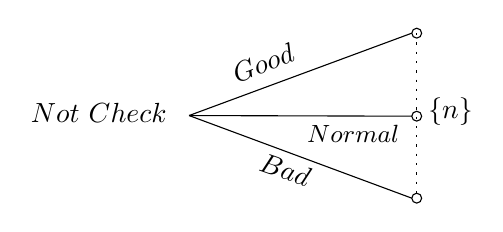
\begin{tikzpicture}[x=0.75pt,y=0.75pt,yscale=-1,xscale=1]
				%uncomment if require: \path (0,300); %set diagram left start at 0, and has height of 300

				%Straight Lines [id:da9949056217510941] 
				\draw    (267.33,117.1) -- (374.63,77.41) ;
				%Straight Lines [id:da0432033074054432] 
				\draw    (267.33,117.1) -- (374.63,156.91) ;
				%Straight Lines [id:da32517464762283166] 
				\draw    (267.33,117.1) -- (374.63,117.41) ;
				%Straight Lines [id:da5711505161730053] 
				\draw  [dash pattern={on 0.84pt off 2.51pt}]  (377,77.41) -- (377,156.91) ;
				%Shape: Circle [id:dp5888816527019345] 
				\draw   (374.63,77.41) .. controls (374.63,76.09) and (375.69,75.03) .. (377,75.03) .. controls (378.31,75.03) and (379.38,76.09) .. (379.38,77.41) .. controls (379.38,78.72) and (378.31,79.78) .. (377,79.78) .. controls (375.69,79.78) and (374.63,78.72) .. (374.63,77.41) -- cycle ;
				%Shape: Circle [id:dp6462591446600507] 
				\draw   (374.63,117.41) .. controls (374.63,116.09) and (375.69,115.03) .. (377,115.03) .. controls (378.31,115.03) and (379.38,116.09) .. (379.38,117.41) .. controls (379.38,118.72) and (378.31,119.78) .. (377,119.78) .. controls (375.69,119.78) and (374.63,118.72) .. (374.63,117.41) -- cycle ;
				%Shape: Circle [id:dp20344233868873163] 
				\draw   (374.63,156.91) .. controls (374.63,155.59) and (375.69,154.53) .. (377,154.53) .. controls (378.31,154.53) and (379.38,155.59) .. (379.38,156.91) .. controls (379.38,158.22) and (378.31,159.28) .. (377,159.28) .. controls (375.69,159.28) and (374.63,158.22) .. (374.63,156.91) -- cycle ;

				% Text Node
				\draw (285.54,92.19) node [anchor=north west][inner sep=0.75pt]  [rotate=-339.07]  {$Good$};
				% Text Node
				\draw (322.98,120.65) node [anchor=north west][inner sep=0.75pt]  [font=\small]  {$Normal$};
				% Text Node
				\draw (189.83,109.7) node [anchor=north west][inner sep=0.75pt]    {$Not\ Check$};
				% Text Node
				\draw (302.77,133.06) node [anchor=north west][inner sep=0.75pt]  [rotate=-19.16]  {$Bad$};
				% Text Node
				\draw (381.33,107.4) node [anchor=north west][inner sep=0.75pt]    {$\{n \}$};


			\end{tikzpicture}
		\end{minipage}
	\end{table}

	\vfill

	Prices both constitute a \textbf{signal} and induce a \textbf{menu} of feasible outcomes.

\end{frame}

\begin{frame}[noframenumbering]{Illustrative Example}

	The investor likes believing the state is good.

	\vfill

	Under \( \textcolor{RoyalBlue}{\overline{p}} \) she distorts the signal to be more positive and overinvests.

	\vfill

	\textbf{Trade-off}: receiving pleasant information but acting under a distorted belief. \pause

	\vfill

	\begin{table}[H]
		\centering
		\begin{minipage}{0.29\textwidth}

		\end{minipage}\hspace{0.3cm} % Adjust the horizontal space between the tables and the symbol
		% Symbol goes here
		\begin{minipage}{0.29\textwidth}
			\centering
			\begin{tikzpicture}[x=0.75pt,y=0.75pt,yscale=-1,xscale=1]
				%uncomment if require: \path (0,341); %set diagram left start at 0, and has height of 341

				%Straight Lines [id:da6521689763503256] 
				\draw [color=RoyalBlue, draw opacity=1]   (259.33,139.1) -- (366.63,99.41) ;
				%Straight Lines [id:da3094065715046459] 
				\draw [color=Red, draw opacity=1]   (259.33,139.1) -- (366.63,178.91) ;
				%Straight Lines [id:da3636097363244992] 
				\draw [color=RoyalBlue, draw opacity=1]   (259.33,139.1) -- (366.63,139.41) ;
				%Straight Lines [id:da7301255340273027] 
				\draw  [dash pattern={on 0.84pt off 2.51pt}]  (369,99.41) -- (369,139.41) ;
				%Shape: Circle [id:dp5572573680385027] 
				\draw   (366.63,99.41) .. controls (366.63,98.09) and (367.69,97.03) .. (369,97.03) .. controls (370.31,97.03) and (371.38,98.09) .. (371.38,99.41) .. controls (371.38,100.72) and (370.31,101.78) .. (369,101.78) .. controls (367.69,101.78) and (366.63,100.72) .. (366.63,99.41) -- cycle ;
				%Shape: Circle [id:dp045414237311399264] 
				\draw   (366.63,139.41) .. controls (366.63,138.09) and (367.69,137.03) .. (369,137.03) .. controls (370.31,137.03) and (371.38,138.09) .. (371.38,139.41) .. controls (371.38,140.72) and (370.31,141.78) .. (369,141.78) .. controls (367.69,141.78) and (366.63,140.72) .. (366.63,139.41) -- cycle ;
				%Shape: Circle [id:dp6206756734194616] 
				\draw   (366.63,178.91) .. controls (366.63,177.59) and (367.69,176.53) .. (369,176.53) .. controls (370.31,176.53) and (371.38,177.59) .. (371.38,178.91) .. controls (371.38,180.22) and (370.31,181.28) .. (369,181.28) .. controls (367.69,181.28) and (366.63,180.22) .. (366.63,178.91) -- cycle ;

				% Text Node
				\draw (277.54,114.19) node [anchor=north west][inner sep=0.75pt]  [color=RoyalBlue ,opacity=1 ,rotate=-339.07]  {$Good$};
				% Text Node
				\draw (314.98,142.65) node [anchor=north west][inner sep=0.75pt]  [font=\small,color=RoyalBlue ,opacity=1 ]  {$Normal$};
				% Text Node
				\draw (211.83,130.7) node [anchor=north west][inner sep=0.75pt]    {$Check$};
				% Text Node
				\draw (294.77,155.06) node [anchor=north west][inner sep=0.75pt]  [color=Red ,opacity=1 ,rotate=-19.16]  {$Bad$};
				% Text Node
				\draw (371.33,156.4) node [anchor=north west][inner sep=0.75pt]  [color=Red ,opacity=1 ]  {$\overset{\underline{p}}{\{i ,n\}}$};
				% Text Node
				\draw (370.83,98.4) node [anchor=north west][inner sep=0.75pt]  [color=RoyalBlue ,opacity=1 ]  {$\overset{\overline{p}}{\{i ,n\}}$};

			\end{tikzpicture}
		\end{minipage}\hspace{2cm} % Adjust the horizontal space between the tables and the symbol
		\( \succ \)
		\begin{minipage}{0.45\textwidth}
			\centering
			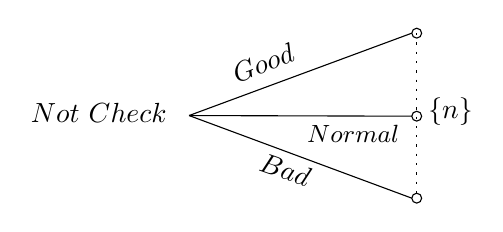
\begin{tikzpicture}[x=0.75pt,y=0.75pt,yscale=-1,xscale=1]
				%uncomment if require: \path (0,300); %set diagram left start at 0, and has height of 300

				%Straight Lines [id:da9949056217510941] 
				\draw    (267.33,117.1) -- (374.63,77.41) ;
				%Straight Lines [id:da0432033074054432] 
				\draw    (267.33,117.1) -- (374.63,156.91) ;
				%Straight Lines [id:da32517464762283166] 
				\draw    (267.33,117.1) -- (374.63,117.41) ;
				%Straight Lines [id:da5711505161730053] 
				\draw  [dash pattern={on 0.84pt off 2.51pt}]  (377,77.41) -- (377,156.91) ;
				%Shape: Circle [id:dp5888816527019345] 
				\draw   (374.63,77.41) .. controls (374.63,76.09) and (375.69,75.03) .. (377,75.03) .. controls (378.31,75.03) and (379.38,76.09) .. (379.38,77.41) .. controls (379.38,78.72) and (378.31,79.78) .. (377,79.78) .. controls (375.69,79.78) and (374.63,78.72) .. (374.63,77.41) -- cycle ;
				%Shape: Circle [id:dp6462591446600507] 
				\draw   (374.63,117.41) .. controls (374.63,116.09) and (375.69,115.03) .. (377,115.03) .. controls (378.31,115.03) and (379.38,116.09) .. (379.38,117.41) .. controls (379.38,118.72) and (378.31,119.78) .. (377,119.78) .. controls (375.69,119.78) and (374.63,118.72) .. (374.63,117.41) -- cycle ;
				%Shape: Circle [id:dp20344233868873163] 
				\draw   (374.63,156.91) .. controls (374.63,155.59) and (375.69,154.53) .. (377,154.53) .. controls (378.31,154.53) and (379.38,155.59) .. (379.38,156.91) .. controls (379.38,158.22) and (378.31,159.28) .. (377,159.28) .. controls (375.69,159.28) and (374.63,158.22) .. (374.63,156.91) -- cycle ;

				% Text Node
				\draw (285.54,92.19) node [anchor=north west][inner sep=0.75pt]  [rotate=-339.07]  {$Good$};
				% Text Node
				\draw (322.98,120.65) node [anchor=north west][inner sep=0.75pt]  [font=\small]  {$Normal$};
				% Text Node
				\draw (189.83,109.7) node [anchor=north west][inner sep=0.75pt]    {$Not\ Check$};
				% Text Node
				\draw (302.77,133.06) node [anchor=north west][inner sep=0.75pt]  [rotate=-19.16]  {$Bad$};
				% Text Node
				\draw (381.33,107.4) node [anchor=north west][inner sep=0.75pt]    {$\{n \}$};


			\end{tikzpicture}
		\end{minipage}
	\end{table}


\end{frame}

\begin{frame}[noframenumbering]{Illustrative Example}

	She might also prefer not to check because she is afraid of the bad signal.

	\vfill

	\begin{table}[H]
		\centering
		\begin{minipage}{0.29\textwidth}

		\end{minipage}\hspace{0.3cm} % Adjust the horizontal space between the tables and the symbol
		% Symbol goes here
		\begin{minipage}{0.29\textwidth}
			\centering
			\begin{tikzpicture}[x=0.75pt,y=0.75pt,yscale=-1,xscale=1]
				%uncomment if require: \path (0,341); %set diagram left start at 0, and has height of 341

				%Straight Lines [id:da6521689763503256] 
				\draw [color=RoyalBlue, draw opacity=1]   (259.33,139.1) -- (366.63,99.41) ;
				%Straight Lines [id:da3094065715046459] 
				\draw [color=Red, draw opacity=1]   (259.33,139.1) -- (366.63,178.91) ;
				%Straight Lines [id:da3636097363244992] 
				\draw [color=RoyalBlue, draw opacity=1]   (259.33,139.1) -- (366.63,139.41) ;
				%Straight Lines [id:da7301255340273027] 
				\draw  [dash pattern={on 0.84pt off 2.51pt}]  (369,99.41) -- (369,139.41) ;
				%Shape: Circle [id:dp5572573680385027] 
				\draw   (366.63,99.41) .. controls (366.63,98.09) and (367.69,97.03) .. (369,97.03) .. controls (370.31,97.03) and (371.38,98.09) .. (371.38,99.41) .. controls (371.38,100.72) and (370.31,101.78) .. (369,101.78) .. controls (367.69,101.78) and (366.63,100.72) .. (366.63,99.41) -- cycle ;
				%Shape: Circle [id:dp045414237311399264] 
				\draw   (366.63,139.41) .. controls (366.63,138.09) and (367.69,137.03) .. (369,137.03) .. controls (370.31,137.03) and (371.38,138.09) .. (371.38,139.41) .. controls (371.38,140.72) and (370.31,141.78) .. (369,141.78) .. controls (367.69,141.78) and (366.63,140.72) .. (366.63,139.41) -- cycle ;
				%Shape: Circle [id:dp6206756734194616] 
				\draw   (366.63,178.91) .. controls (366.63,177.59) and (367.69,176.53) .. (369,176.53) .. controls (370.31,176.53) and (371.38,177.59) .. (371.38,178.91) .. controls (371.38,180.22) and (370.31,181.28) .. (369,181.28) .. controls (367.69,181.28) and (366.63,180.22) .. (366.63,178.91) -- cycle ;

				% Text Node
				\draw (277.54,114.19) node [anchor=north west][inner sep=0.75pt]  [color=RoyalBlue ,opacity=1 ,rotate=-339.07]  {$Good$};
				% Text Node
				\draw (314.98,142.65) node [anchor=north west][inner sep=0.75pt]  [font=\small,color=RoyalBlue ,opacity=1 ]  {$Normal$};
				% Text Node
				\draw (211.83,130.7) node [anchor=north west][inner sep=0.75pt]    {$Check$};
				% Text Node
				\draw (294.77,155.06) node [anchor=north west][inner sep=0.75pt]  [color=Red ,opacity=1 ,rotate=-19.16]  {$Bad$};
				% Text Node
				\draw (371.33,156.4) node [anchor=north west][inner sep=0.75pt]  [color=Red ,opacity=1 ]  {$\overset{\underline{p}}{\{i ,n\}}$};
				% Text Node
				\draw (370.83,98.4) node [anchor=north west][inner sep=0.75pt]  [color=RoyalBlue ,opacity=1 ]  {$\overset{\overline{p}}{\{i ,n\}}$};

			\end{tikzpicture}
		\end{minipage}\hspace{2cm} % Adjust the horizontal space between the tables and the symbol
		\( \prec  \)
		\begin{minipage}{0.45\textwidth}
			\centering
			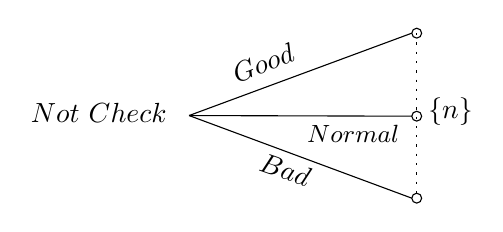
\begin{tikzpicture}[x=0.75pt,y=0.75pt,yscale=-1,xscale=1]
				%uncomment if require: \path (0,300); %set diagram left start at 0, and has height of 300

				%Straight Lines [id:da9949056217510941] 
				\draw    (267.33,117.1) -- (374.63,77.41) ;
				%Straight Lines [id:da0432033074054432] 
				\draw    (267.33,117.1) -- (374.63,156.91) ;
				%Straight Lines [id:da32517464762283166] 
				\draw    (267.33,117.1) -- (374.63,117.41) ;
				%Straight Lines [id:da5711505161730053] 
				\draw  [dash pattern={on 0.84pt off 2.51pt}]  (377,77.41) -- (377,156.91) ;
				%Shape: Circle [id:dp5888816527019345] 
				\draw   (374.63,77.41) .. controls (374.63,76.09) and (375.69,75.03) .. (377,75.03) .. controls (378.31,75.03) and (379.38,76.09) .. (379.38,77.41) .. controls (379.38,78.72) and (378.31,79.78) .. (377,79.78) .. controls (375.69,79.78) and (374.63,78.72) .. (374.63,77.41) -- cycle ;
				%Shape: Circle [id:dp6462591446600507] 
				\draw   (374.63,117.41) .. controls (374.63,116.09) and (375.69,115.03) .. (377,115.03) .. controls (378.31,115.03) and (379.38,116.09) .. (379.38,117.41) .. controls (379.38,118.72) and (378.31,119.78) .. (377,119.78) .. controls (375.69,119.78) and (374.63,118.72) .. (374.63,117.41) -- cycle ;
				%Shape: Circle [id:dp20344233868873163] 
				\draw   (374.63,156.91) .. controls (374.63,155.59) and (375.69,154.53) .. (377,154.53) .. controls (378.31,154.53) and (379.38,155.59) .. (379.38,156.91) .. controls (379.38,158.22) and (378.31,159.28) .. (377,159.28) .. controls (375.69,159.28) and (374.63,158.22) .. (374.63,156.91) -- cycle ;

				% Text Node
				\draw (285.54,92.19) node [anchor=north west][inner sep=0.75pt]  [rotate=-339.07]  {$Good$};
				% Text Node
				\draw (322.98,120.65) node [anchor=north west][inner sep=0.75pt]  [font=\small]  {$Normal$};
				% Text Node
				\draw (189.83,109.7) node [anchor=north west][inner sep=0.75pt]    {$Not\ Check$};
				% Text Node
				\draw (302.77,133.06) node [anchor=north west][inner sep=0.75pt]  [rotate=-19.16]  {$Bad$};
				% Text Node
				\draw (381.33,107.4) node [anchor=north west][inner sep=0.75pt]    {$\{n \}$};


			\end{tikzpicture}
		\end{minipage}
		%\caption{Excessive investment.} % Add your caption here
		%\label{tab:excess}
	\end{table} \pause

	\vfill

	Both excessive trading and the ostrich effect constitute empirical puzzles in finance \citep{danielOverconfidentInvestorsPredictable2015,golmanInformationAvoidance2017}.

\end{frame}

\begin{frame}[noframenumbering]{Illustrative Example}

	\textbf{Variant}: commit not to invest, e.g. by delegating to a financial advisor or algorithm.

	\vfill

	\begin{table}[H]
		\centering
		\begin{minipage}{0.29\textwidth}

		\end{minipage}\hspace{0.3cm} % Adjust the horizontal space between the tables and the symbol
		% Symbol goes here
		\begin{minipage}{0.29\textwidth}
			\centering
			\begin{tikzpicture}[x=0.75pt,y=0.75pt,yscale=-1,xscale=1]
				%uncomment if require: \path (0,341); %set diagram left start at 0, and has height of 341

				%Straight Lines [id:da6521689763503256] 
				\draw [color=RoyalBlue, draw opacity=1]   (259.33,139.1) -- (366.63,99.41) ;
				%Straight Lines [id:da3094065715046459] 
				\draw [color=Red, draw opacity=1]   (259.33,139.1) -- (366.63,178.91) ;
				%Straight Lines [id:da3636097363244992] 
				\draw [color=RoyalBlue, draw opacity=1]   (259.33,139.1) -- (366.63,139.41) ;
				%Straight Lines [id:da7301255340273027] 
				\draw  [dash pattern={on 0.84pt off 2.51pt}]  (369,99.41) -- (369,139.41) ;
				%Shape: Circle [id:dp5572573680385027] 
				\draw   (366.63,99.41) .. controls (366.63,98.09) and (367.69,97.03) .. (369,97.03) .. controls (370.31,97.03) and (371.38,98.09) .. (371.38,99.41) .. controls (371.38,100.72) and (370.31,101.78) .. (369,101.78) .. controls (367.69,101.78) and (366.63,100.72) .. (366.63,99.41) -- cycle ;
				%Shape: Circle [id:dp045414237311399264] 
				\draw   (366.63,139.41) .. controls (366.63,138.09) and (367.69,137.03) .. (369,137.03) .. controls (370.31,137.03) and (371.38,138.09) .. (371.38,139.41) .. controls (371.38,140.72) and (370.31,141.78) .. (369,141.78) .. controls (367.69,141.78) and (366.63,140.72) .. (366.63,139.41) -- cycle ;
				%Shape: Circle [id:dp6206756734194616] 
				\draw   (366.63,178.91) .. controls (366.63,177.59) and (367.69,176.53) .. (369,176.53) .. controls (370.31,176.53) and (371.38,177.59) .. (371.38,178.91) .. controls (371.38,180.22) and (370.31,181.28) .. (369,181.28) .. controls (367.69,181.28) and (366.63,180.22) .. (366.63,178.91) -- cycle ;

				% Text Node
				\draw (277.54,114.19) node [anchor=north west][inner sep=0.75pt]  [color=RoyalBlue ,opacity=1 ,rotate=-339.07]  {$Good$};
				% Text Node
				\draw (314.98,142.65) node [anchor=north west][inner sep=0.75pt]  [font=\small,color=RoyalBlue ,opacity=1 ]  {$Normal$};
				% Text Node
				\draw (203.83,130.7) node [anchor=north west][inner sep=0.75pt]    {$Delegate$};
				% Text Node
				\draw (294.77,155.06) node [anchor=north west][inner sep=0.75pt]  [color=Red ,opacity=1 ,rotate=-19.16]  {$Bad$};
				% Text Node
				\draw (371.33,156.4) node [anchor=north west][inner sep=0.75pt]  [color=Red ,opacity=1 ]  {$\overset{\underline{p}}{\{n\}}$};
				% Text Node
				\draw (370.83,98.4) node [anchor=north west][inner sep=0.75pt]  [color=RoyalBlue ,opacity=1 ]  {$\overset{\overline{p}}{\{n\}}$};

			\end{tikzpicture}
		\end{minipage}\hspace{2cm} % Adjust the horizontal space between the tables and the symbol
		\begin{minipage}{0.45\textwidth}
			\centering
			\begin{tikzpicture}[x=0.75pt,y=0.75pt,yscale=-1,xscale=1]
				%uncomment if require: \path (0,341); %set diagram left start at 0, and has height of 341

				%Straight Lines [id:da6521689763503256] 
				\draw [color=RoyalBlue, draw opacity=1]   (259.33,139.1) -- (366.63,99.41) ;
				%Straight Lines [id:da3094065715046459] 
				\draw [color=Red, draw opacity=1]   (259.33,139.1) -- (366.63,178.91) ;
				%Straight Lines [id:da3636097363244992] 
				\draw [color=RoyalBlue, draw opacity=1]   (259.33,139.1) -- (366.63,139.41) ;
				%Straight Lines [id:da7301255340273027] 
				\draw  [dash pattern={on 0.84pt off 2.51pt}]  (369,99.41) -- (369,139.41) ;
				%Shape: Circle [id:dp5572573680385027] 
				\draw   (366.63,99.41) .. controls (366.63,98.09) and (367.69,97.03) .. (369,97.03) .. controls (370.31,97.03) and (371.38,98.09) .. (371.38,99.41) .. controls (371.38,100.72) and (370.31,101.78) .. (369,101.78) .. controls (367.69,101.78) and (366.63,100.72) .. (366.63,99.41) -- cycle ;
				%Shape: Circle [id:dp045414237311399264] 
				\draw   (366.63,139.41) .. controls (366.63,138.09) and (367.69,137.03) .. (369,137.03) .. controls (370.31,137.03) and (371.38,138.09) .. (371.38,139.41) .. controls (371.38,140.72) and (370.31,141.78) .. (369,141.78) .. controls (367.69,141.78) and (366.63,140.72) .. (366.63,139.41) -- cycle ;
				%Shape: Circle [id:dp6206756734194616] 
				\draw   (366.63,178.91) .. controls (366.63,177.59) and (367.69,176.53) .. (369,176.53) .. controls (370.31,176.53) and (371.38,177.59) .. (371.38,178.91) .. controls (371.38,180.22) and (370.31,181.28) .. (369,181.28) .. controls (367.69,181.28) and (366.63,180.22) .. (366.63,178.91) -- cycle ;

				% Text Node
				\draw (277.54,114.19) node [anchor=north west][inner sep=0.75pt]  [color=RoyalBlue ,opacity=1 ,rotate=-339.07]  {$Good$};
				% Text Node
				\draw (314.98,142.65) node [anchor=north west][inner sep=0.75pt]  [font=\small,color=RoyalBlue ,opacity=1 ]  {$Normal$};
				% Text Node
				\draw (211.83,130.7) node [anchor=north west][inner sep=0.75pt]    {$Check$};
				% Text Node
				\draw (294.77,155.06) node [anchor=north west][inner sep=0.75pt]  [color=Red ,opacity=1 ,rotate=-19.16]  {$Bad$};
				% Text Node
				\draw (371.33,156.4) node [anchor=north west][inner sep=0.75pt]  [color=Red ,opacity=1 ]  {$\overset{\underline{p}}{\{i ,n\}}$};
				% Text Node
				\draw (370.83,98.4) node [anchor=north west][inner sep=0.75pt]  [color=RoyalBlue ,opacity=1 ]  {$\overset{\overline{p}}{\{i ,n\}}$};

			\end{tikzpicture}
		\end{minipage}
		%\caption{Excessive investment.} % Add your caption here
		%\label{tab:excess}
	\end{table} \pause

	\vfill

	\textbf{Trade-off}: receiving pleasant information but \sout{acting under a distorted belief}.

\end{frame}

\begin{frame}[noframenumbering]{Illustrative Example}
	\textbf{Solution}: commit not to invest, e.g. by delegating to a financial advisor or algorithm.

	\vfill

	\begin{table}[H]
		\centering
		\begin{minipage}{0.29\textwidth}

		\end{minipage}\hspace{0.3cm} % Adjust the horizontal space between the tables and the symbol
		% Symbol goes here
		\begin{minipage}{0.29\textwidth}
			\centering
			\begin{tikzpicture}[x=0.75pt,y=0.75pt,yscale=-1,xscale=1]
				%uncomment if require: \path (0,341); %set diagram left start at 0, and has height of 341

				%Straight Lines [id:da6521689763503256] 
				\draw [color=RoyalBlue, draw opacity=1]   (259.33,139.1) -- (366.63,99.41) ;
				%Straight Lines [id:da3094065715046459] 
				\draw [color=Red, draw opacity=1]   (259.33,139.1) -- (366.63,178.91) ;
				%Straight Lines [id:da3636097363244992] 
				\draw [color=RoyalBlue, draw opacity=1]   (259.33,139.1) -- (366.63,139.41) ;
				%Straight Lines [id:da7301255340273027] 
				\draw  [dash pattern={on 0.84pt off 2.51pt}]  (369,99.41) -- (369,139.41) ;
				%Shape: Circle [id:dp5572573680385027] 
				\draw   (366.63,99.41) .. controls (366.63,98.09) and (367.69,97.03) .. (369,97.03) .. controls (370.31,97.03) and (371.38,98.09) .. (371.38,99.41) .. controls (371.38,100.72) and (370.31,101.78) .. (369,101.78) .. controls (367.69,101.78) and (366.63,100.72) .. (366.63,99.41) -- cycle ;
				%Shape: Circle [id:dp045414237311399264] 
				\draw   (366.63,139.41) .. controls (366.63,138.09) and (367.69,137.03) .. (369,137.03) .. controls (370.31,137.03) and (371.38,138.09) .. (371.38,139.41) .. controls (371.38,140.72) and (370.31,141.78) .. (369,141.78) .. controls (367.69,141.78) and (366.63,140.72) .. (366.63,139.41) -- cycle ;
				%Shape: Circle [id:dp6206756734194616] 
				\draw   (366.63,178.91) .. controls (366.63,177.59) and (367.69,176.53) .. (369,176.53) .. controls (370.31,176.53) and (371.38,177.59) .. (371.38,178.91) .. controls (371.38,180.22) and (370.31,181.28) .. (369,181.28) .. controls (367.69,181.28) and (366.63,180.22) .. (366.63,178.91) -- cycle ;

				% Text Node
				\draw (277.54,114.19) node [anchor=north west][inner sep=0.75pt]  [color=RoyalBlue ,opacity=1 ,rotate=-339.07]  {$Good$};
				% Text Node
				\draw (314.98,142.65) node [anchor=north west][inner sep=0.75pt]  [font=\small,color=RoyalBlue ,opacity=1 ]  {$Normal$};
				% Text Node
				\draw (203.83,130.7) node [anchor=north west][inner sep=0.75pt]    {$Delegate$};
				% Text Node
				\draw (294.77,155.06) node [anchor=north west][inner sep=0.75pt]  [color=Red ,opacity=1 ,rotate=-19.16]  {$Bad$};
				% Text Node
				\draw (371.33,156.4) node [anchor=north west][inner sep=0.75pt]  [color=Red ,opacity=1 ]  {$\overset{\underline{p}}{\{n\}}$};
				% Text Node
				\draw (370.83,98.4) node [anchor=north west][inner sep=0.75pt]  [color=RoyalBlue ,opacity=1 ]  {$\overset{\overline{p}}{\{n\}}$};

			\end{tikzpicture}
		\end{minipage}\hspace{2cm} % Adjust the horizontal space between the tables and the symbol
		\( \succ \)
		\begin{minipage}{0.45\textwidth}
			\centering
			\begin{tikzpicture}[x=0.75pt,y=0.75pt,yscale=-1,xscale=1]
				%uncomment if require: \path (0,341); %set diagram left start at 0, and has height of 341

				%Straight Lines [id:da6521689763503256] 
				\draw [color=RoyalBlue, draw opacity=1]   (259.33,139.1) -- (366.63,99.41) ;
				%Straight Lines [id:da3094065715046459] 
				\draw [color=Red, draw opacity=1]   (259.33,139.1) -- (366.63,178.91) ;
				%Straight Lines [id:da3636097363244992] 
				\draw [color=RoyalBlue, draw opacity=1]   (259.33,139.1) -- (366.63,139.41) ;
				%Straight Lines [id:da7301255340273027] 
				\draw  [dash pattern={on 0.84pt off 2.51pt}]  (369,99.41) -- (369,139.41) ;
				%Shape: Circle [id:dp5572573680385027] 
				\draw   (366.63,99.41) .. controls (366.63,98.09) and (367.69,97.03) .. (369,97.03) .. controls (370.31,97.03) and (371.38,98.09) .. (371.38,99.41) .. controls (371.38,100.72) and (370.31,101.78) .. (369,101.78) .. controls (367.69,101.78) and (366.63,100.72) .. (366.63,99.41) -- cycle ;
				%Shape: Circle [id:dp045414237311399264] 
				\draw   (366.63,139.41) .. controls (366.63,138.09) and (367.69,137.03) .. (369,137.03) .. controls (370.31,137.03) and (371.38,138.09) .. (371.38,139.41) .. controls (371.38,140.72) and (370.31,141.78) .. (369,141.78) .. controls (367.69,141.78) and (366.63,140.72) .. (366.63,139.41) -- cycle ;
				%Shape: Circle [id:dp6206756734194616] 
				\draw   (366.63,178.91) .. controls (366.63,177.59) and (367.69,176.53) .. (369,176.53) .. controls (370.31,176.53) and (371.38,177.59) .. (371.38,178.91) .. controls (371.38,180.22) and (370.31,181.28) .. (369,181.28) .. controls (367.69,181.28) and (366.63,180.22) .. (366.63,178.91) -- cycle ;

				% Text Node
				\draw (277.54,114.19) node [anchor=north west][inner sep=0.75pt]  [color=RoyalBlue ,opacity=1 ,rotate=-339.07]  {$Good$};
				% Text Node
				\draw (314.98,142.65) node [anchor=north west][inner sep=0.75pt]  [font=\small,color=RoyalBlue ,opacity=1 ]  {$Normal$};
				% Text Node
				\draw (211.83,130.7) node [anchor=north west][inner sep=0.75pt]    {$Check$};
				% Text Node
				\draw (294.77,155.06) node [anchor=north west][inner sep=0.75pt]  [color=Red ,opacity=1 ,rotate=-19.16]  {$Bad$};
				% Text Node
				\draw (371.33,156.4) node [anchor=north west][inner sep=0.75pt]  [color=Red ,opacity=1 ]  {$\overset{\underline{p}}{\{i ,n\}}$};
				% Text Node
				\draw (370.83,98.4) node [anchor=north west][inner sep=0.75pt]  [color=RoyalBlue ,opacity=1 ]  {$\overset{\overline{p}}{\{i ,n\}}$};

			\end{tikzpicture}
		\end{minipage}
		%\caption{Excessive investment.} % Add your caption here
		%\label{tab:excess}
	\end{table}

	\vfill

	\textbf{Trade-off}: receiving pleasant information but \sout{acting under a distorted belief}.

	\vfill

	Commitment might be welfare enhancing under belief-dependent preferences.

\end{frame}

\section{Comparison with the literature}

\begin{frame}\frametitle{Literature}

	\begin{wideitemize}
		\item \textit{Decision Theory.} \cite{liangInformationdependentExpectedUtility2017}, \cite{dillenbergerAdditivebeliefbasedPreferences2020} \cite{rommeswinkelPreferenceKnowledge2023}.

		\vspace{0.3cm}
		\underline{Contribution}: \textbf{Belief revision rule, identification}.
		\item \textit{Menu Choice.} \cite{gulTemptationSelfControl2001}, \cite{ozdenorenCompletingStateSpace2002}, \cite{epsteinAxiomaticModelNonBayesian2006}, \cite{epsteinColdFeet2007}.

		\vspace{0.3cm}
		\underline{Contribution}: \textbf{Novel primitive object of choice}.
		\item \textit{Belief-Dependent Preferences.} \cite{brunnermeierOptimalExpectations2005}, \cite{eliazCanAnticipatoryFeelings2006}, \cite{benabou2016mindful}, \cite{golmanInformationAvoidance2017}, \cite{battigalliBeliefdependentMotivationsPsychological2022}.

		\vspace{0.3cm}
		\underline{Contribution}: \textbf{Generality, derivation of belief revision rule, identification}.
	\end{wideitemize}

\end{frame}

\section{Full model}

\begin{frame}{Model: acts}

	\tikzset{every picture/.style={line width=0.75pt}} %set default line width to 0.75pt        

	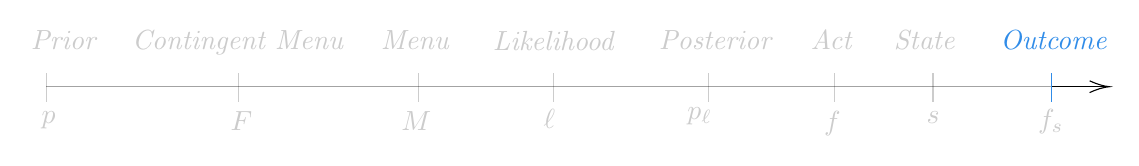
\begin{tikzpicture}[x=0.65pt,y=0.65pt,yscale=-1,xscale=1]
		% Uncomment if required: \path (0,472); % Set diagram left start at 0, and has height of 472

		% Draw the transparent horizontal line (arrow)
		\draw[opacity=0.2] (23,250) -- (614,250);

		% Draw the part of the horizontal arrow to the left of the vertical segment in transparent
		\draw[opacity=0.2] (23,250) -- (582,250);

		% Draw the part of the horizontal arrow to the right of the vertical segment in black
		\draw[black] (582,250) -- (614,250);

		% Draw the black oblique segments at the end of the horizontal arrow (pointing left)
		\draw[black, shift={(614,250)}, rotate=180]
		(10.93,-3.29) .. controls (6.95,-1.4) and (3.31,-0.3) .. (0,0) .. controls (3.31,0.3) and (6.95,1.4) .. (10.93,3.29);

		% Draw the small vertical segments below each word
		\draw[opacity=0.2] (23,242.5) -- (23,258.5);
		\draw[opacity=0.2] (130,242.5) -- (130,258.5);
		\draw[opacity=0.2] (230,242.5) -- (230,258.5);
		\draw[opacity=0.2] (305,242.5) -- (305,258.5);
		\draw[opacity=0.2] (391,242.5) -- (391,258.5);
		\draw[opacity=0.2] (461,242.5) -- (461,258.5);
		\draw[opacity=0.2] (516,242.5) -- (516,258.5);

		% The vertical segment below "Outcome" in RoyalBlue
		\draw[opacity=1, RoyalBlue] (582,242.5) -- (582,258.5);

		% Text for symbols (bottom) with reduced opacity
		\draw[opacity=0.2] (124,262.15) node [anchor=north west][inner sep=0.75pt] {\( F \)};
		\draw[opacity=0.2] (219,262.15) node [anchor=north west][inner sep=0.75pt] {\(M\)};
		\draw[opacity=0.2] (378,260.15) node [anchor=north west][inner sep=0.75pt] {\(p_{\ell}\)};
		\draw[opacity=0.2] (511,262.15) node [anchor=north west][inner sep=0.75pt] {\(s\)};
		\draw[opacity=0.2] (573,261.15) node [anchor=north west][inner sep=0.75pt] {\(f_{s}\)};
		\draw[opacity=0.2] (454,262.15) node [anchor=north west][inner sep=0.75pt] {\(f\)};
		\draw[opacity=0.2] (298,261.15) node [anchor=north west][inner sep=0.75pt] {\(\ell\)};
		\draw[opacity=0.2] (19,262.15) node [anchor=north west][inner sep=0.75pt] {\(p\)};

		% Text for labels (top) with reduced opacity
		\draw[opacity=0.2] (69.29,217.5) node [anchor=north west][inner sep=0.75pt] [align=left] {\textit{Contingent Menu}};
		\draw[opacity=0.2] (207.58,217.5) node [anchor=north west][inner sep=0.75pt] [align=left] {\textit{Menu}};
		\draw[opacity=0.2] (362.16,217.5) node [anchor=north west][inner sep=0.75pt] [align=left] {\textit{Posterior}};
		\draw[opacity=0.2] (492.74,217.5) node [anchor=north west][inner sep=0.75pt] [align=left] {\textit{State}};
		\draw[opacity=0.2] (446.45,217.5) node [anchor=north west][inner sep=0.75pt] [align=left] {\textit{Act}};
		\draw[opacity=0.2] (269.87,217.5) node [anchor=north west][inner sep=0.75pt] [align=left] {\textit{Likelihood}};
		\draw[opacity=0.2] (13,217.5) node [anchor=north west][inner sep=0.75pt] [align=left] {\textit{Prior}};

		% The word "Outcome" in RoyalBlue
		\draw[opacity=1, RoyalBlue] (552,217.5) node [anchor=north west][inner sep=0.75pt] [align=left] {\textit{Outcome}};
	\end{tikzpicture}

	\vfill

	\begin{columns}
		% Left Column (adjusted width and smaller table font)
		\begin{column}{0.45\textwidth}  % Increased width slightly to 0.45\textwidth
			\begin{center}
				%\scriptsize  % Reduces the font size inside the table
				\begin{table}[H]
					\centering


					\tikzset{every picture/.style={line width=0.75pt}} %set default line width to 0.75pt        

					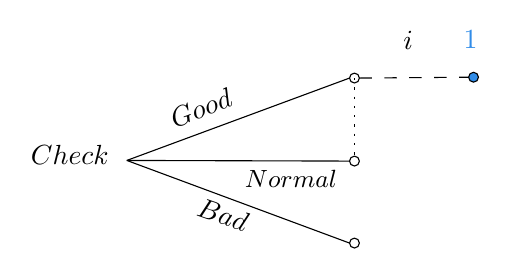
\begin{tikzpicture}[x=0.75pt,y=0.75pt,yscale=-1,xscale=1]
						%uncomment if require: \path (0,300); %set diagram left start at 0, and has height of 300

						%Straight Lines [id:da218161262308447] 
						\draw [color={rgb, 255:red, 0; green, 0; blue, 0 }  ,draw opacity=1 ]   (242.33,112.1) -- (349.63,72.41) ;
						%Straight Lines [id:da7719682575310538] 
						\draw [color={rgb, 255:red, 0; green, 0; blue, 0 }  ,draw opacity=1 ]   (242.33,112.1) -- (349.63,151.91) ;
						%Straight Lines [id:da24594340319254204] 
						\draw [color={rgb, 255:red, 0; green, 0; blue, 0 }  ,draw opacity=1 ]   (242.33,112.1) -- (349.63,112.41) ;
						%Straight Lines [id:da312275016958093] 
						\draw  [dash pattern={on 0.84pt off 2.51pt}]  (352,72.41) -- (352,112.41) ;
						%Shape: Circle [id:dp971111480899022] 
						\draw   (349.63,72.41) .. controls (349.63,71.09) and (350.69,70.03) .. (352,70.03) .. controls (353.31,70.03) and (354.38,71.09) .. (354.38,72.41) .. controls (354.38,73.72) and (353.31,74.78) .. (352,74.78) .. controls (350.69,74.78) and (349.63,73.72) .. (349.63,72.41) -- cycle ;
						%Shape: Circle [id:dp2636421863386722] 
						\draw   (349.63,112.41) .. controls (349.63,111.09) and (350.69,110.03) .. (352,110.03) .. controls (353.31,110.03) and (354.38,111.09) .. (354.38,112.41) .. controls (354.38,113.72) and (353.31,114.78) .. (352,114.78) .. controls (350.69,114.78) and (349.63,113.72) .. (349.63,112.41) -- cycle ;
						%Shape: Circle [id:dp4223499111750235] 
						\draw   (349.63,151.91) .. controls (349.63,150.59) and (350.69,149.53) .. (352,149.53) .. controls (353.31,149.53) and (354.38,150.59) .. (354.38,151.91) .. controls (354.38,153.22) and (353.31,154.28) .. (352,154.28) .. controls (350.69,154.28) and (349.63,153.22) .. (349.63,151.91) -- cycle ;
						%Straight Lines [id:da7454925496732656] 
						\draw  [dash pattern={on 4.5pt off 4.5pt}]  (354.38,72.41) -- (407,72) ;
						%Shape: Circle [id:dp1890835149928527] 
						\draw  [fill=RoyalBlue ,fill opacity=1 ] (407,72) .. controls (407,70.69) and (408.06,69.63) .. (409.38,69.63) .. controls (410.69,69.63) and (411.75,70.69) .. (411.75,72) .. controls (411.75,73.31) and (410.69,74.38) .. (409.38,74.38) .. controls (408.06,74.38) and (407,73.31) .. (407,72) -- cycle ;

						% Text Node
						\draw (260.54,87.19) node [anchor=north west][inner sep=0.75pt]  [color={rgb, 255:red, 0; green, 0; blue, 0 }  ,opacity=1 ,rotate=-339.07]  {$Good$};
						% Text Node
						\draw (297.98,115.65) node [anchor=north west][inner sep=0.75pt]  [font=\small,color={rgb, 255:red, 0; green, 0; blue, 0 }  ,opacity=1 ]  {$Normal$};
						% Text Node
						\draw (194.83,103.7) node [anchor=north west][inner sep=0.75pt]    {$Check$};
						% Text Node
						\draw (277.77,128.06) node [anchor=north west][inner sep=0.75pt]  [color={rgb, 255:red, 0; green, 0; blue, 0 }  ,opacity=1 ,rotate=-19.16]  {$Bad$};
						% Text Node
						\draw (374.33,48.4) node [anchor=north west][inner sep=0.75pt]  [color={rgb, 255:red, 0; green, 0; blue, 0 }  ,opacity=1 ]  {$i$};
						% Text Node
						\draw (403.33,48.4) node [anchor=north west][inner sep=0.75pt]  [color={rgb, 255:red, 0; green, 0; blue, 0 }  ,opacity=1 ]  {$\textcolor{RoyalBlue}{1}$};

					\end{tikzpicture}
				\end{table}
			\end{center}
		\end{column}

		% Right Column (slightly reduced width)
		\begin{column}{0.55\textwidth}  % Adjusted right column to 0.55\textwidth
			\begin{itemize}
				\item \textcolor{RoyalBlue}{outcome} set (net financial return);
			\end{itemize}
		\end{column}
	\end{columns}

\end{frame}

\begin{frame}[noframenumbering]{Model: acts}

	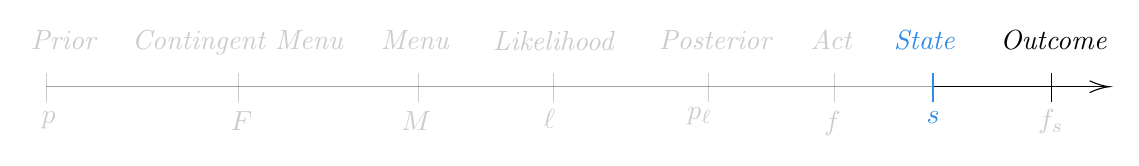
\begin{tikzpicture}[x=0.65pt,y=0.65pt,yscale=-1,xscale=1]
		% Uncomment if required: \path (0,472); % Set diagram left start at 0, and has height of 472

		% Draw the transparent horizontal line (arrow)
		\draw[opacity=0.2] (23,250) -- (614,250);

		% Draw the part of the horizontal arrow to the left of the vertical segment in transparent
		\draw[opacity=0.2] (23,250) -- (582,250);

		% Draw the part of the horizontal arrow to the right of the vertical segment in black
		\draw[black] (516,250) -- (614,250);

		% Draw the black oblique segments at the end of the horizontal arrow (pointing left)
		\draw[black, shift={(614,250)}, rotate=180]
		(10.93,-3.29) .. controls (6.95,-1.4) and (3.31,-0.3) .. (0,0) .. controls (3.31,0.3) and (6.95,1.4) .. (10.93,3.29);

		% Draw the small vertical segments below each word
		\draw[opacity=0.2] (23,242.5) -- (23,258.5);
		\draw[opacity=0.2] (130,242.5) -- (130,258.5);
		\draw[opacity=0.2] (230,242.5) -- (230,258.5);
		\draw[opacity=0.2] (305,242.5) -- (305,258.5);
		\draw[opacity=0.2] (391,242.5) -- (391,258.5);
		\draw[opacity=0.2] (461,242.5) -- (461,258.5);

		% The vertical segment below "Outcome" in black
		\draw[black] (582,242.5) -- (582,258.5);

		% The word "Outcome" in black
		\draw[opacity=1, black] (552,217.5) node [anchor=north west][inner sep=0.75pt] [align=left] {\textit{Outcome}};

		% The vertical segment below "State" in RoyalBlue
		\draw[opacity=1, RoyalBlue] (516,242.5) -- (516,258.5);

		% The word "State" in RoyalBlue
		\draw[opacity=1, RoyalBlue] (492.74,217.5) node [anchor=north west][inner sep=0.75pt] [align=left] {\textit{State}};

		% The symbol "s" in RoyalBlue
		\draw[opacity=1, RoyalBlue] (511,262.15) node [anchor=north west][inner sep=0.75pt] {\(s\)};

		% Text for symbols (bottom) with reduced opacity
		\draw[opacity=0.2] (124,262.15) node [anchor=north west][inner sep=0.75pt] {\( F \)};
		\draw[opacity=0.2] (219,262.15) node [anchor=north west][inner sep=0.75pt] {\(M\)};
		\draw[opacity=0.2] (378,260.15) node [anchor=north west][inner sep=0.75pt] {\(p_{\ell}\)};
		\draw[opacity=0.2] (573,261.15) node [anchor=north west][inner sep=0.75pt] {\(f_{s}\)};
		\draw[opacity=0.2] (454,262.15) node [anchor=north west][inner sep=0.75pt] {\(f\)};
		\draw[opacity=0.2] (298,261.15) node [anchor=north west][inner sep=0.75pt] {\(\ell\)};
		\draw[opacity=0.2] (19,262.15) node [anchor=north west][inner sep=0.75pt] {\(p\)};

		% Text for labels (top) with reduced opacity
		\draw[opacity=0.2] (69.29,217.5) node [anchor=north west][inner sep=0.75pt] [align=left] {\textit{Contingent Menu}};
		\draw[opacity=0.2] (207.58,217.5) node [anchor=north west][inner sep=0.75pt] [align=left] {\textit{Menu}};
		\draw[opacity=0.2] (362.16,217.5) node [anchor=north west][inner sep=0.75pt] [align=left] {\textit{Posterior}};
		\draw[opacity=0.2] (446.45,217.5) node [anchor=north west][inner sep=0.75pt] [align=left] {\textit{Act}};
		\draw[opacity=0.2] (269.87,217.5) node [anchor=north west][inner sep=0.75pt] [align=left] {\textit{Likelihood}};
		\draw[opacity=0.2] (13,217.5) node [anchor=north west][inner sep=0.75pt] [align=left] {\textit{Prior}};
	\end{tikzpicture}


	\vfill

	\begin{columns}
		% Left Column (adjusted width and smaller table font)
		\begin{column}{0.45\textwidth}  % Increased width slightly to 0.45\textwidth
			\begin{center}
				%\scriptsize  % Reduces the font size inside the table
				\begin{table}[H]
					\centering
					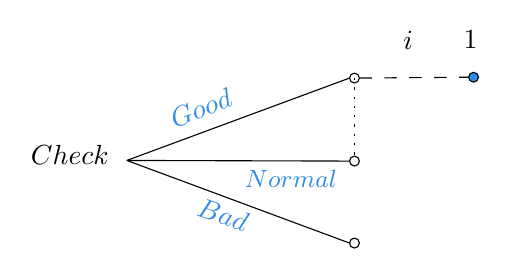
\begin{tikzpicture}[x=0.75pt,y=0.75pt,yscale=-1,xscale=1]
						%uncomment if require: \path (0,300); %set diagram left start at 0, and has height of 300

						%Straight Lines [id:da218161262308447] 
						\draw [color={rgb, 255:red, 0; green, 0; blue, 0 }  ,draw opacity=1 ]   (242.33,112.1) -- (349.63,72.41) ;
						%Straight Lines [id:da7719682575310538] 
						\draw [color={rgb, 255:red, 0; green, 0; blue, 0 }  ,draw opacity=1 ]   (242.33,112.1) -- (349.63,151.91) ;
						%Straight Lines [id:da24594340319254204] 
						\draw [color={rgb, 255:red, 0; green, 0; blue, 0 }  ,draw opacity=1 ]   (242.33,112.1) -- (349.63,112.41) ;
						%Straight Lines [id:da312275016958093] 
						\draw  [dash pattern={on 0.84pt off 2.51pt}]  (352,72.41) -- (352,112.41) ;
						%Shape: Circle [id:dp971111480899022] 
						\draw   (349.63,72.41) .. controls (349.63,71.09) and (350.69,70.03) .. (352,70.03) .. controls (353.31,70.03) and (354.38,71.09) .. (354.38,72.41) .. controls (354.38,73.72) and (353.31,74.78) .. (352,74.78) .. controls (350.69,74.78) and (349.63,73.72) .. (349.63,72.41) -- cycle ;
						%Shape: Circle [id:dp2636421863386722] 
						\draw   (349.63,112.41) .. controls (349.63,111.09) and (350.69,110.03) .. (352,110.03) .. controls (353.31,110.03) and (354.38,111.09) .. (354.38,112.41) .. controls (354.38,113.72) and (353.31,114.78) .. (352,114.78) .. controls (350.69,114.78) and (349.63,113.72) .. (349.63,112.41) -- cycle ;
						%Shape: Circle [id:dp4223499111750235] 
						\draw   (349.63,151.91) .. controls (349.63,150.59) and (350.69,149.53) .. (352,149.53) .. controls (353.31,149.53) and (354.38,150.59) .. (354.38,151.91) .. controls (354.38,153.22) and (353.31,154.28) .. (352,154.28) .. controls (350.69,154.28) and (349.63,153.22) .. (349.63,151.91) -- cycle ;
						%Straight Lines [id:da7454925496732656] 
						\draw  [dash pattern={on 4.5pt off 4.5pt}]  (354.38,72.41) -- (407,72) ;
						%Shape: Circle [id:dp1890835149928527] 
						\draw  [fill=RoyalBlue ,fill opacity=1 ] (407,72) .. controls (407,70.69) and (408.06,69.63) .. (409.38,69.63) .. controls (410.69,69.63) and (411.75,70.69) .. (411.75,72) .. controls (411.75,73.31) and (410.69,74.38) .. (409.38,74.38) .. controls (408.06,74.38) and (407,73.31) .. (407,72) -- cycle ;

						% Text Node
						\draw (260.54,87.19) node [anchor=north west][inner sep=0.75pt]  [color={rgb, 255:red, 0; green, 0; blue, 0 }  ,opacity=1 ,rotate=-339.07]  {$\textcolor{RoyalBlue}{Good}$};
						% Text Node
						\draw (297.98,115.65) node [anchor=north west][inner sep=0.75pt]  [font=\small,color={rgb, 255:red, 0; green, 0; blue, 0 }  ,opacity=1 ]  {$\textcolor{RoyalBlue}{Normal}$};
						% Text Node
						\draw (194.83,103.7) node [anchor=north west][inner sep=0.75pt]    {$Check$};
						% Text Node
						\draw (277.77,128.06) node [anchor=north west][inner sep=0.75pt]  [color={rgb, 255:red, 0; green, 0; blue, 0 }  ,opacity=1 ,rotate=-19.16]  {$\textcolor{RoyalBlue}{Bad}$};
						% Text Node
						\draw (374.33,48.4) node [anchor=north west][inner sep=0.75pt]  [color={rgb, 255:red, 0; green, 0; blue, 0 }  ,opacity=1 ]  {$i$};
						% Text Node
						\draw (403.33,48.4) node [anchor=north west][inner sep=0.75pt]  [color={rgb, 255:red, 0; green, 0; blue, 0 }  ,opacity=1 ]  {$1$};

					\end{tikzpicture}
				\end{table}
			\end{center}
		\end{column}

		% Right Column (slightly reduced width)
		\begin{column}{0.55\textwidth}  % Adjusted right column to 0.55\textwidth
			\begin{itemize}
				\item outcome set;
				\item \textcolor{RoyalBlue}{state} set;
			\end{itemize}
		\end{column}
	\end{columns}

\end{frame}

\begin{frame}[noframenumbering]{Model: acts}

	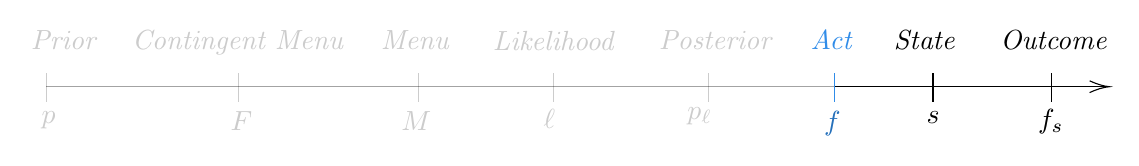
\begin{tikzpicture}[x=0.65pt,y=0.65pt,yscale=-1,xscale=1]
		% Uncomment if required: \path (0,472); % Set diagram left start at 0, and has height of 472

		% Draw the transparent horizontal line (arrow)
		\draw[opacity=0.2] (23,250) -- (614,250);

		% Draw the part of the horizontal arrow to the left of the vertical segment in transparent
		\draw[opacity=0.2] (23,250) -- (582,250);

		% Draw the part of the horizontal arrow to the right of the vertical segment in black
		\draw[black] (461,250) -- (614,250);

		% Draw the black oblique segments at the end of the horizontal arrow (pointing left)
		\draw[black, shift={(614,250)}, rotate=180]
		(10.93,-3.29) .. controls (6.95,-1.4) and (3.31,-0.3) .. (0,0) .. controls (3.31,0.3) and (6.95,1.4) .. (10.93,3.29);

		% Draw the small vertical segments below each word
		\draw[opacity=0.2] (23,242.5) -- (23,258.5);
		\draw[opacity=0.2] (130,242.5) -- (130,258.5);
		\draw[opacity=0.2] (230,242.5) -- (230,258.5);
		\draw[opacity=0.2] (305,242.5) -- (305,258.5);
		\draw[opacity=0.2] (391,242.5) -- (391,258.5);

		% The vertical segment below "Outcome, State" in black
		\draw[black] (582,242.5) -- (582,258.5);
		\draw[black] (516,242.5) -- (516,258.5);

		% The word "Outcome, State" in black
		\draw[opacity=1, black] (552,217.5) node [anchor=north west][inner sep=0.75pt] [align=left] {\textit{Outcome}};
		\draw[opacity=1, black] (492.74,217.5) node [anchor=north west][inner sep=0.75pt] [align=left] {\textit{State}};

		% The vertical segment below "Act" in RoyalBlue
		\draw[opacity=1, RoyalBlue] (461,242.5) -- (461,258.5);

		% The word "Act" in RoyalBlue
		\draw[opacity=1, RoyalBlue] (446.45,217.5) node [anchor=north west][inner sep=0.75pt] [align=left] {\textit{Act}};

		% The symbol "s, f_s" in black
		\draw[opacity=1, black] (511,262.15) node [anchor=north west][inner sep=0.75pt] {\(s\)};
		\draw[opacity=1, black] (573,261.15) node [anchor=north west][inner sep=0.75pt] {\(f_{s}\)};

		% The symbol "f" in RoyalBlue
		\draw[opacity=1, RoyalBlue] (454,262.15) node [anchor=north west][inner sep=0.75pt] {\(f\)};

		% Text for symbols (bottom) with reduced opacity
		\draw[opacity=0.2] (124,262.15) node [anchor=north west][inner sep=0.75pt] {\( F \)};
		\draw[opacity=0.2] (219,262.15) node [anchor=north west][inner sep=0.75pt] {\(M\)};
		\draw[opacity=0.2] (378,260.15) node [anchor=north west][inner sep=0.75pt] {\(p_{\ell}\)};
		\draw[opacity=0.2] (573,261.15) node [anchor=north west][inner sep=0.75pt] {\(f_{s}\)};
		\draw[opacity=0.2] (454,262.15) node [anchor=north west][inner sep=0.75pt] {\(f\)};
		\draw[opacity=0.2] (298,261.15) node [anchor=north west][inner sep=0.75pt] {\(\ell\)};
		\draw[opacity=0.2] (19,262.15) node [anchor=north west][inner sep=0.75pt] {\(p\)};

		% Text for labels (top) with reduced opacity
		\draw[opacity=0.2] (69.29,217.5) node [anchor=north west][inner sep=0.75pt] [align=left] {\textit{Contingent Menu}};
		\draw[opacity=0.2] (207.58,217.5) node [anchor=north west][inner sep=0.75pt] [align=left] {\textit{Menu}};
		\draw[opacity=0.2] (362.16,217.5) node [anchor=north west][inner sep=0.75pt] [align=left] {\textit{Posterior}};
		\draw[opacity=0.2] (269.87,217.5) node [anchor=north west][inner sep=0.75pt] [align=left] {\textit{Likelihood}};
		\draw[opacity=0.2] (13,217.5) node [anchor=north west][inner sep=0.75pt] [align=left] {\textit{Prior}};
	\end{tikzpicture}

	\vfill

	\begin{columns}
		% Left Column (adjusted width and smaller table font)
		\begin{column}{0.45\textwidth}  % Increased width slightly to 0.45\textwidth
			\begin{center}
				%\scriptsize  % Reduces the font size inside the table
				\begin{table}[H]
					\centering
					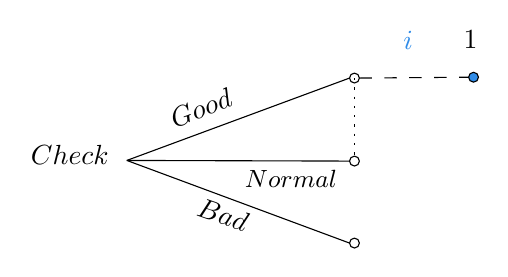
\begin{tikzpicture}[x=0.75pt,y=0.75pt,yscale=-1,xscale=1]
						%uncomment if require: \path (0,300); %set diagram left start at 0, and has height of 300

						%Straight Lines [id:da218161262308447] 
						\draw [color={rgb, 255:red, 0; green, 0; blue, 0 }  ,draw opacity=1 ]   (242.33,112.1) -- (349.63,72.41) ;
						%Straight Lines [id:da7719682575310538] 
						\draw [color={rgb, 255:red, 0; green, 0; blue, 0 }  ,draw opacity=1 ]   (242.33,112.1) -- (349.63,151.91) ;
						%Straight Lines [id:da24594340319254204] 
						\draw [color={rgb, 255:red, 0; green, 0; blue, 0 }  ,draw opacity=1 ]   (242.33,112.1) -- (349.63,112.41) ;
						%Straight Lines [id:da312275016958093] 
						\draw  [dash pattern={on 0.84pt off 2.51pt}]  (352,72.41) -- (352,112.41) ;
						%Shape: Circle [id:dp971111480899022] 
						\draw   (349.63,72.41) .. controls (349.63,71.09) and (350.69,70.03) .. (352,70.03) .. controls (353.31,70.03) and (354.38,71.09) .. (354.38,72.41) .. controls (354.38,73.72) and (353.31,74.78) .. (352,74.78) .. controls (350.69,74.78) and (349.63,73.72) .. (349.63,72.41) -- cycle ;
						%Shape: Circle [id:dp2636421863386722] 
						\draw   (349.63,112.41) .. controls (349.63,111.09) and (350.69,110.03) .. (352,110.03) .. controls (353.31,110.03) and (354.38,111.09) .. (354.38,112.41) .. controls (354.38,113.72) and (353.31,114.78) .. (352,114.78) .. controls (350.69,114.78) and (349.63,113.72) .. (349.63,112.41) -- cycle ;
						%Shape: Circle [id:dp4223499111750235] 
						\draw   (349.63,151.91) .. controls (349.63,150.59) and (350.69,149.53) .. (352,149.53) .. controls (353.31,149.53) and (354.38,150.59) .. (354.38,151.91) .. controls (354.38,153.22) and (353.31,154.28) .. (352,154.28) .. controls (350.69,154.28) and (349.63,153.22) .. (349.63,151.91) -- cycle ;
						%Straight Lines [id:da7454925496732656] 
						\draw  [dash pattern={on 4.5pt off 4.5pt}]  (354.38,72.41) -- (407,72) ;
						%Shape: Circle [id:dp1890835149928527] 
						\draw  [fill=RoyalBlue ,fill opacity=1 ] (407,72) .. controls (407,70.69) and (408.06,69.63) .. (409.38,69.63) .. controls (410.69,69.63) and (411.75,70.69) .. (411.75,72) .. controls (411.75,73.31) and (410.69,74.38) .. (409.38,74.38) .. controls (408.06,74.38) and (407,73.31) .. (407,72) -- cycle ;

						% Text Node
						\draw (260.54,87.19) node [anchor=north west][inner sep=0.75pt]  [color={rgb, 255:red, 0; green, 0; blue, 0 }  ,opacity=1 ,rotate=-339.07]  {$Good$};
						% Text Node
						\draw (297.98,115.65) node [anchor=north west][inner sep=0.75pt]  [font=\small,color={rgb, 255:red, 0; green, 0; blue, 0 }  ,opacity=1 ]  {$Normal$};
						% Text Node
						\draw (194.83,103.7) node [anchor=north west][inner sep=0.75pt]    {$Check$};
						% Text Node
						\draw (277.77,128.06) node [anchor=north west][inner sep=0.75pt]  [color={rgb, 255:red, 0; green, 0; blue, 0 }  ,opacity=1 ,rotate=-19.16]  {$Bad$};
						% Text Node
						\draw (374.33,48.4) node [anchor=north west][inner sep=0.75pt]  [color={rgb, 255:red, 0; green, 0; blue, 0 }  ,opacity=1 ]  {$\textcolor{RoyalBlue}{i}$};
						% Text Node
						\draw (403.33,48.4) node [anchor=north west][inner sep=0.75pt]  [color={rgb, 255:red, 0; green, 0; blue, 0 }  ,opacity=1 ]  {$1$};

					\end{tikzpicture}

				\end{table}
			\end{center}
		\end{column}

		% Right Column (slightly reduced width)
		\begin{column}{0.55\textwidth}  % Adjusted right column to 0.55\textwidth
			\begin{itemize}
				\item outcome set;
				\item state set;
				\item \textcolor{RoyalBlue}{acts} \( f : \: States \: \rightarrow \: Outcomes \);
			\end{itemize}
		\end{column}
	\end{columns}

\end{frame}

\begin{frame}{Model: menus and contingent menus}

	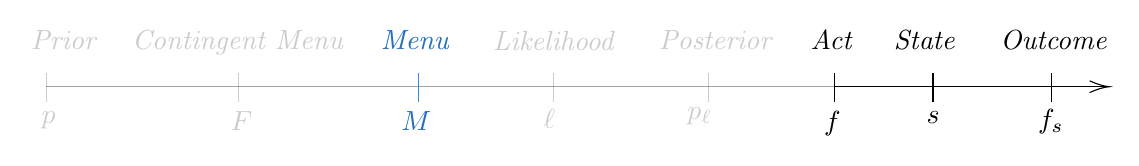
\begin{tikzpicture}[x=0.65pt,y=0.65pt,yscale=-1,xscale=1]
		% Uncomment if required: \path (0,472); % Set diagram left start at 0, and has height of 472

		% Draw the transparent horizontal line (arrow)
		\draw[opacity=0.2] (23,250) -- (614,250);

		% Draw the part of the horizontal arrow to the left of the vertical segment in transparent
		\draw[opacity=0.2] (23,250) -- (582,250);

		% Draw the part of the horizontal arrow to the right of the vertical segment in black
		\draw[black] (461,250) -- (614,250);

		% Draw the black oblique segments at the end of the horizontal arrow (pointing left)
		\draw[black, shift={(614,250)}, rotate=180]
		(10.93,-3.29) .. controls (6.95,-1.4) and (3.31,-0.3) .. (0,0) .. controls (3.31,0.3) and (6.95,1.4) .. (10.93,3.29);

		% Draw the small vertical segments below each word
		\draw[opacity=0.2] (23,242.5) -- (23,258.5);
		\draw[opacity=0.2] (130,242.5) -- (130,258.5);
		\draw[opacity=0.2] (230,242.5) -- (230,258.5);
		\draw[opacity=0.2] (305,242.5) -- (305,258.5);
		\draw[opacity=0.2] (391,242.5) -- (391,258.5);

		% The vertical segment below "Outcome, State, Act" in black
		\draw[black] (582,242.5) -- (582,258.5);
		\draw[black] (516,242.5) -- (516,258.5);
		\draw[black] (461,242.5) -- (461,258.5);

		% The word "Outcome, State, Act" in black
		\draw[opacity=1, black] (552,217.5) node [anchor=north west][inner sep=0.75pt] [align=left] {\textit{Outcome}};
		\draw[opacity=1, black] (492.74,217.5) node [anchor=north west][inner sep=0.75pt] [align=left] {\textit{State}};
		\draw[opacity=1, black] (446.45,217.5) node [anchor=north west][inner sep=0.75pt] [align=left] {\textit{Act}};

		% The vertical segment below "Menu" in RoyalBlue
		\draw[opacity=1, RoyalBlue] (230,242.5) -- (230,258.5);

		% The word "Menu" in RoyalBlue
		\draw[opacity=1, RoyalBlue] (207.58,217.5) node [anchor=north west][inner sep=0.75pt] [align=left] {\textit{Menu}};

		% The symbol "s, f_s, f" in black
		\draw[opacity=1, black] (511,262.15) node [anchor=north west][inner sep=0.75pt] {\(s\)};
		\draw[opacity=1, black] (573,261.15) node [anchor=north west][inner sep=0.75pt] {\(f_{s}\)};
		\draw[opacity=1, black] (454,262.15) node [anchor=north west][inner sep=0.75pt] {\(f\)};

		% The symbol "M" in RoyalBlue
		\draw[opacity=1, RoyalBlue] (219,262.15) node [anchor=north west][inner sep=0.75pt] {\(M\)};

		% Text for symbols (bottom) with reduced opacity
		\draw[opacity=0.2] (124,262.15) node [anchor=north west][inner sep=0.75pt] {\( F \)};
		\draw[opacity=0.2] (219,262.15) node [anchor=north west][inner sep=0.75pt] {\(M\)};
		\draw[opacity=0.2] (378,260.15) node [anchor=north west][inner sep=0.75pt] {\(p_{\ell}\)};
		\draw[opacity=0.2] (573,261.15) node [anchor=north west][inner sep=0.75pt] {\(f_{s}\)};
		\draw[opacity=0.2] (454,262.15) node [anchor=north west][inner sep=0.75pt] {\(f\)};
		\draw[opacity=0.2] (298,261.15) node [anchor=north west][inner sep=0.75pt] {\(\ell\)};
		\draw[opacity=0.2] (19,262.15) node [anchor=north west][inner sep=0.75pt] {\(p\)};

		% Text for labels (top) with reduced opacity
		\draw[opacity=0.2] (69.29,217.5) node [anchor=north west][inner sep=0.75pt] [align=left] {\textit{Contingent Menu}};
		\draw[opacity=0.2] (207.58,217.5) node [anchor=north west][inner sep=0.75pt] [align=left] {\textit{Menu}};
		\draw[opacity=0.2] (362.16,217.5) node [anchor=north west][inner sep=0.75pt] [align=left] {\textit{Posterior}};
		\draw[opacity=0.2] (269.87,217.5) node [anchor=north west][inner sep=0.75pt] [align=left] {\textit{Likelihood}};
		\draw[opacity=0.2] (13,217.5) node [anchor=north west][inner sep=0.75pt] [align=left] {\textit{Prior}};
	\end{tikzpicture}

	\vfill

	\begin{columns}
		% Left Column (adjusted width and smaller table font)
		\begin{column}{0.45\textwidth}  % Increased width slightly to 0.45\textwidth
			\begin{center}
				%\scriptsize  % Reduces the font size inside the table
				\begin{table}[H]
					\centering
					\begin{tikzpicture}[x=0.75pt,y=0.75pt,yscale=-1,xscale=1]
						%uncomment if require: \path (0,300); %set diagram left start at 0, and has height of 300

						%Straight Lines [id:da10589365900996173] 
						\draw [color={rgb, 255:red, 0; green, 0; blue, 0 }  ,draw opacity=1 ]   (262.33,132.1) -- (369.63,92.41) ;
						%Straight Lines [id:da5796893993758667] 
						\draw [color={rgb, 255:red, 0; green, 0; blue, 0 }  ,draw opacity=1 ]   (262.33,132.1) -- (369.63,171.91) ;
						%Straight Lines [id:da024405781766148493] 
						\draw [color={rgb, 255:red, 0; green, 0; blue, 0 }  ,draw opacity=1 ]   (262.33,132.1) -- (369.63,132.41) ;
						%Straight Lines [id:da569061638772357] 
						\draw  [dash pattern={on 0.84pt off 2.51pt}]  (372,94.78) -- (372,130.03) ;
						%Shape: Circle [id:dp5199064102665634] 
						\draw   (369.63,92.41) .. controls (369.63,91.09) and (370.69,90.03) .. (372,90.03) .. controls (373.31,90.03) and (374.38,91.09) .. (374.38,92.41) .. controls (374.38,93.72) and (373.31,94.78) .. (372,94.78) .. controls (370.69,94.78) and (369.63,93.72) .. (369.63,92.41) -- cycle ;
						%Shape: Circle [id:dp7343244546600616] 
						\draw   (369.63,132.41) .. controls (369.63,131.09) and (370.69,130.03) .. (372,130.03) .. controls (373.31,130.03) and (374.38,131.09) .. (374.38,132.41) .. controls (374.38,133.72) and (373.31,134.78) .. (372,134.78) .. controls (370.69,134.78) and (369.63,133.72) .. (369.63,132.41) -- cycle ;
						%Shape: Circle [id:dp8289076341983612] 
						\draw   (369.63,171.91) .. controls (369.63,170.59) and (370.69,169.53) .. (372,169.53) .. controls (373.31,169.53) and (374.38,170.59) .. (374.38,171.91) .. controls (374.38,173.22) and (373.31,174.28) .. (372,174.28) .. controls (370.69,174.28) and (369.63,173.22) .. (369.63,171.91) -- cycle ;

						% Text Node
						\draw (280.54,107.19) node [anchor=north west][inner sep=0.75pt]  [color={rgb, 255:red, 0; green, 0; blue, 0 }  ,opacity=1 ,rotate=-339.07]  {$Good$};
						% Text Node
						\draw (317.98,135.65) node [anchor=north west][inner sep=0.75pt]  [font=\small,color={rgb, 255:red, 0; green, 0; blue, 0 }  ,opacity=1 ]  {$Normal$};
						% Text Node
						\draw (214.83,123.7) node [anchor=north west][inner sep=0.75pt]    {$Check$};
						% Text Node
						\draw (297.77,148.06) node [anchor=north west][inner sep=0.75pt]  [color={rgb, 255:red, 0; green, 0; blue, 0 }  ,opacity=1 ,rotate=-19.16]  {$Bad$};
						% Text Node
						\draw (375.33,150.4) node [anchor=north west][inner sep=0.75pt]  [color=Black ,opacity=1 ]  {$\overset{\underline{p}}{\{i ,n\}}$};
						% Text Node
						\draw (375.75,95.4) node [anchor=north west][inner sep=0.75pt]  [color=Black ,opacity=1 ]  {$\textcolor{RoyalBlue}{\overset{\overline{p}}{\{i ,n\}}}$};
					\end{tikzpicture}
				\end{table}
			\end{center}
		\end{column}

		% Right Column (slightly reduced width)
		\begin{column}{0.55\textwidth}  % Adjusted right column to 0.55\textwidth
			\begin{itemize}
				\item outcome set;
				\item state set;
				\item acts \( f : \: States \: \rightarrow \: Outcomes \);
				\item a set of acts is a \textcolor{RoyalBlue}{menu} \( M \);
			\end{itemize}
		\end{column}
	\end{columns}

\end{frame}

\begin{frame}[noframenumbering]{Model: menus and contingent menus}

	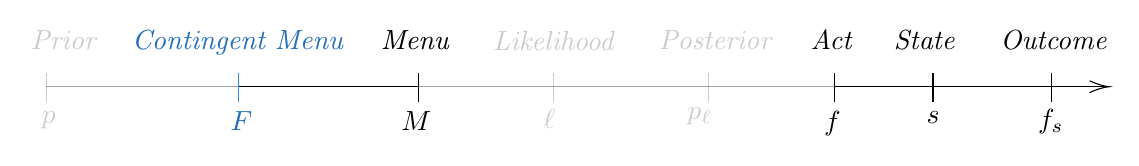
\begin{tikzpicture}[x=0.65pt,y=0.65pt,yscale=-1,xscale=1]
		% Uncomment if required: \path (0,472); % Set diagram left start at 0, and has height of 472

		% Draw the transparent horizontal line (arrow)
		\draw[opacity=0.2] (23,250) -- (614,250);

		% Draw the part of the horizontal arrow to the left of the vertical segment in transparent
		\draw[opacity=0.2] (23,250) -- (582,250);

		% Draw the part of the horizontal arrow to the right of the vertical segment in black
		\draw[black] (130,250) -- (230,250);
		\draw[black] (461,250) -- (614,250);

		% Draw the black oblique segments at the end of the horizontal arrow (pointing left)
		\draw[black, shift={(614,250)}, rotate=180]
		(10.93,-3.29) .. controls (6.95,-1.4) and (3.31,-0.3) .. (0,0) .. controls (3.31,0.3) and (6.95,1.4) .. (10.93,3.29);

		% Draw the small vertical segments below each word
		\draw[opacity=0.2] (23,242.5) -- (23,258.5);
		\draw[opacity=0.2] (130,242.5) -- (130,258.5);
		\draw[opacity=0.2] (230,242.5) -- (230,258.5);
		\draw[opacity=0.2] (305,242.5) -- (305,258.5);
		\draw[opacity=0.2] (391,242.5) -- (391,258.5);

		% The vertical segment below "Outcome, State, Act, Menu" in black
		\draw[black] (582,242.5) -- (582,258.5);
		\draw[black] (516,242.5) -- (516,258.5);
		\draw[black] (461,242.5) -- (461,258.5);
		\draw[black] (230,242.5) -- (230,258.5);

		% The word "Outcome, State, Act, Menu" in black
		\draw[opacity=1, black] (552,217.5) node [anchor=north west][inner sep=0.75pt] [align=left] {\textit{Outcome}};
		\draw[opacity=1, black] (492.74,217.5) node [anchor=north west][inner sep=0.75pt] [align=left] {\textit{State}};
		\draw[opacity=1, black] (446.45,217.5) node [anchor=north west][inner sep=0.75pt] [align=left] {\textit{Act}};
		\draw[opacity=1, black] (207.58,217.5) node [anchor=north west][inner sep=0.75pt] [align=left] {\textit{Menu}};

		% The vertical segment below "Contingent Menu" in RoyalBlue
		\draw[opacity=1, RoyalBlue] (130,242.5) -- (130,258.5);

		% The word "Contingent Menu" in RoyalBlue
		\draw[opacity=1, RoyalBlue] (69.29,217.5) node [anchor=north west][inner sep=0.75pt] [align=left] {\textit{Contingent Menu}};

		% The symbol "s, f_s, f, M" in black
		\draw[opacity=1, black] (511,262.15) node [anchor=north west][inner sep=0.75pt] {\(s\)};
		\draw[opacity=1, black] (573,261.15) node [anchor=north west][inner sep=0.75pt] {\(f_{s}\)};
		\draw[opacity=1, black] (454,262.15) node [anchor=north west][inner sep=0.75pt] {\(f\)};
		\draw[opacity=1, black] (219,262.15) node [anchor=north west][inner sep=0.75pt] {\(M\)};

		% The symbol "F" in RoyalBlue
		\draw[opacity=1, RoyalBlue] (124,262.15) node [anchor=north west][inner sep=0.75pt] {\( F \)};

		% Text for symbols (bottom) with reduced opacity
		\draw[opacity=0.2] (124,262.15) node [anchor=north west][inner sep=0.75pt] {\( F \)};
		\draw[opacity=0.2] (378,260.15) node [anchor=north west][inner sep=0.75pt] {\(p_{\ell}\)};
		\draw[opacity=0.2] (298,261.15) node [anchor=north west][inner sep=0.75pt] {\(\ell\)};
		\draw[opacity=0.2] (19,262.15) node [anchor=north west][inner sep=0.75pt] {\(p\)};

		% Text for labels (top) with reduced opacity
		\draw[opacity=0.2] (69.29,217.5) node [anchor=north west][inner sep=0.75pt] [align=left] {\textit{Contingent Menu}};
		\draw[opacity=0.2] (207.58,217.5) node [anchor=north west][inner sep=0.75pt] [align=left] {\textit{Menu}};
		\draw[opacity=0.2] (362.16,217.5) node [anchor=north west][inner sep=0.75pt] [align=left] {\textit{Posterior}};
		\draw[opacity=0.2] (269.87,217.5) node [anchor=north west][inner sep=0.75pt] [align=left] {\textit{Likelihood}};
		\draw[opacity=0.2] (13,217.5) node [anchor=north west][inner sep=0.75pt] [align=left] {\textit{Prior}};
	\end{tikzpicture}

	\vfill

	\begin{columns}
		% Left Column (adjusted width and smaller table font)
		\begin{column}{0.45\textwidth}  % Increased width slightly to 0.45\textwidth
			\begin{center}
				\begin{table}[H]
					\centering
					\begin{tikzpicture}[x=0.75pt,y=0.75pt,yscale=-1,xscale=1]
						%uncomment if require: \path (0,300); %set diagram left start at 0, and has height of 300

						%Straight Lines [id:da10589365900996173] 
						\draw [color={rgb, 255:red, 0; green, 0; blue, 0 }  ,draw opacity=1 ]   (262.33,132.1) -- (369.63,92.41) ;
						%Straight Lines [id:da5796893993758667] 
						\draw [color={rgb, 255:red, 0; green, 0; blue, 0 }  ,draw opacity=1 ]   (262.33,132.1) -- (369.63,171.91) ;
						%Straight Lines [id:da024405781766148493] 
						\draw [color={rgb, 255:red, 0; green, 0; blue, 0 }  ,draw opacity=1 ]   (262.33,132.1) -- (369.63,132.41) ;
						%Straight Lines [id:da569061638772357] 
						\draw  [dash pattern={on 0.84pt off 2.51pt}]  (372,94.78) -- (372,130.03) ;
						%Shape: Circle [id:dp5199064102665634] 
						\draw   (369.63,92.41) .. controls (369.63,91.09) and (370.69,90.03) .. (372,90.03) .. controls (373.31,90.03) and (374.38,91.09) .. (374.38,92.41) .. controls (374.38,93.72) and (373.31,94.78) .. (372,94.78) .. controls (370.69,94.78) and (369.63,93.72) .. (369.63,92.41) -- cycle ;
						%Shape: Circle [id:dp7343244546600616] 
						\draw   (369.63,132.41) .. controls (369.63,131.09) and (370.69,130.03) .. (372,130.03) .. controls (373.31,130.03) and (374.38,131.09) .. (374.38,132.41) .. controls (374.38,133.72) and (373.31,134.78) .. (372,134.78) .. controls (370.69,134.78) and (369.63,133.72) .. (369.63,132.41) -- cycle ;
						%Shape: Circle [id:dp8289076341983612] 
						\draw   (369.63,171.91) .. controls (369.63,170.59) and (370.69,169.53) .. (372,169.53) .. controls (373.31,169.53) and (374.38,170.59) .. (374.38,171.91) .. controls (374.38,173.22) and (373.31,174.28) .. (372,174.28) .. controls (370.69,174.28) and (369.63,173.22) .. (369.63,171.91) -- cycle ;

						% Text Node
						\draw (280.54,107.19) node [anchor=north west][inner sep=0.75pt]  [color={rgb, 255:red, 0; green, 0; blue, 0 }  ,opacity=1 ,rotate=-339.07]  {$Good$};
						% Text Node
						\draw (317.98,135.65) node [anchor=north west][inner sep=0.75pt]  [font=\small,color={rgb, 255:red, 0; green, 0; blue, 0 }  ,opacity=1 ]  {$Normal$};
						% Text Node
						\draw (214.83,123.7) node [anchor=north west][inner sep=0.75pt]    {$\textcolor{RoyalBlue}{Check}$};
						% Text Node
						\draw (297.77,148.06) node [anchor=north west][inner sep=0.75pt]  [color={rgb, 255:red, 0; green, 0; blue, 0 }  ,opacity=1 ,rotate=-19.16]  {$Bad$};
						% Text Node
						\draw (375.33,150.4) node [anchor=north west][inner sep=0.75pt]  [color=Black ,opacity=1 ]  {$\overset{\underline{p}}{\{i ,n\}}$};
						% Text Node
						\draw (375.75,95.4) node [anchor=north west][inner sep=0.75pt]  [color=Black ,opacity=1 ]  {$\overset{\overline{p}}{\{i ,n\}}$};
					\end{tikzpicture}
				\end{table}
			\end{center}
		\end{column}

		% Right Column (slightly reduced width)
		\begin{column}{0.55\textwidth}  % Adjusted right column to 0.55\textwidth
			\begin{itemize}
				\item outcome set;
				\item state set;
				\item acts \( f : \: States \: \rightarrow \: Outcomes \);
				\item a set of acts is a menu \( M \);
				\item a \textcolor{RoyalBlue}{contingent menu} is \(F: States \: \rightarrow \: Menus \).
			\end{itemize}
		\end{column}
	\end{columns}

\end{frame}

\begin{frame}{Model: Information}

	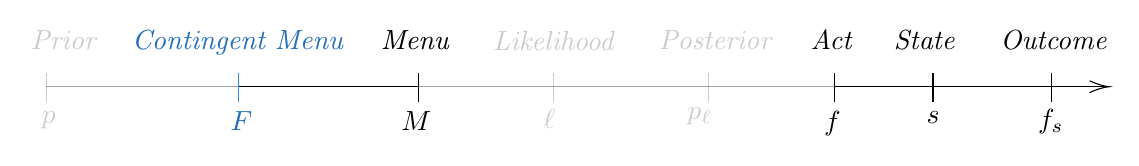
\begin{tikzpicture}[x=0.65pt,y=0.65pt,yscale=-1,xscale=1]
		% Uncomment if required: \path (0,472); % Set diagram left start at 0, and has height of 472

		% Draw the transparent horizontal line (arrow)
		\draw[opacity=0.2] (23,250) -- (614,250);

		% Draw the part of the horizontal arrow to the left of the vertical segment in transparent
		\draw[opacity=0.2] (23,250) -- (582,250);

		% Draw the part of the horizontal arrow to the right of the vertical segment in black
		\draw[black] (130,250) -- (230,250);
		\draw[black] (461,250) -- (614,250);

		% Draw the black oblique segments at the end of the horizontal arrow (pointing left)
		\draw[black, shift={(614,250)}, rotate=180]
		(10.93,-3.29) .. controls (6.95,-1.4) and (3.31,-0.3) .. (0,0) .. controls (3.31,0.3) and (6.95,1.4) .. (10.93,3.29);

		% Draw the small vertical segments below each word
		\draw[opacity=0.2] (23,242.5) -- (23,258.5);
		\draw[opacity=0.2] (130,242.5) -- (130,258.5);
		\draw[opacity=0.2] (230,242.5) -- (230,258.5);
		\draw[opacity=0.2] (305,242.5) -- (305,258.5);
		\draw[opacity=0.2] (391,242.5) -- (391,258.5);

		% The vertical segment below "Outcome, State, Act, Menu" in black
		\draw[black] (582,242.5) -- (582,258.5);
		\draw[black] (516,242.5) -- (516,258.5);
		\draw[black] (461,242.5) -- (461,258.5);
		\draw[black] (230,242.5) -- (230,258.5);

		% The word "Outcome, State, Act, Menu" in black
		\draw[opacity=1, black] (552,217.5) node [anchor=north west][inner sep=0.75pt] [align=left] {\textit{Outcome}};
		\draw[opacity=1, black] (492.74,217.5) node [anchor=north west][inner sep=0.75pt] [align=left] {\textit{State}};
		\draw[opacity=1, black] (446.45,217.5) node [anchor=north west][inner sep=0.75pt] [align=left] {\textit{Act}};
		\draw[opacity=1, black] (207.58,217.5) node [anchor=north west][inner sep=0.75pt] [align=left] {\textit{Menu}};

		% The vertical segment below "Contingent Menu" in RoyalBlue
		\draw[opacity=1, RoyalBlue] (130,242.5) -- (130,258.5);

		% The word "Contingent Menu" in RoyalBlue
		\draw[opacity=1, RoyalBlue] (69.29,217.5) node [anchor=north west][inner sep=0.75pt] [align=left] {\textit{Contingent Menu}};

		% The symbol "s, f_s, f, M" in black
		\draw[opacity=1, black] (511,262.15) node [anchor=north west][inner sep=0.75pt] {\(s\)};
		\draw[opacity=1, black] (573,261.15) node [anchor=north west][inner sep=0.75pt] {\(f_{s}\)};
		\draw[opacity=1, black] (454,262.15) node [anchor=north west][inner sep=0.75pt] {\(f\)};
		\draw[opacity=1, black] (219,262.15) node [anchor=north west][inner sep=0.75pt] {\(M\)};

		% The symbol "F" in RoyalBlue
		\draw[opacity=1, RoyalBlue] (124,262.15) node [anchor=north west][inner sep=0.75pt] {\( F \)};

		% Text for symbols (bottom) with reduced opacity
		\draw[opacity=0.2] (124,262.15) node [anchor=north west][inner sep=0.75pt] {\( F \)};
		\draw[opacity=0.2] (378,260.15) node [anchor=north west][inner sep=0.75pt] {\(p_{\ell}\)};
		\draw[opacity=0.2] (298,261.15) node [anchor=north west][inner sep=0.75pt] {\(\ell\)};
		\draw[opacity=0.2] (19,262.15) node [anchor=north west][inner sep=0.75pt] {\(p\)};

		% Text for labels (top) with reduced opacity
		\draw[opacity=0.2] (69.29,217.5) node [anchor=north west][inner sep=0.75pt] [align=left] {\textit{Contingent Menu}};
		\draw[opacity=0.2] (207.58,217.5) node [anchor=north west][inner sep=0.75pt] [align=left] {\textit{Menu}};
		\draw[opacity=0.2] (362.16,217.5) node [anchor=north west][inner sep=0.75pt] [align=left] {\textit{Posterior}};
		\draw[opacity=0.2] (269.87,217.5) node [anchor=north west][inner sep=0.75pt] [align=left] {\textit{Likelihood}};
		\draw[opacity=0.2] (13,217.5) node [anchor=north west][inner sep=0.75pt] [align=left] {\textit{Prior}};
	\end{tikzpicture}

	\vfill

	\begin{columns}
		% Left Column (adjusted width)
		\begin{column}{0.35\textwidth} % Reduced width to make room for the right column
			\begin{center}
				\begin{table}
					\centering
					\begin{tikzpicture}[x=0.75pt,y=0.75pt,yscale=-1,xscale=1]
						%uncomment if require: \path (0,300); %set diagram left start at 0, and has height of 300

						%Straight Lines [id:da10589365900996173] 
						\draw [color={rgb, 255:red, 0; green, 0; blue, 0 }  ,draw opacity=1 ]   (262.33,132.1) -- (369.63,92.41) ;
						%Straight Lines [id:da5796893993758667] 
						\draw [color={rgb, 255:red, 0; green, 0; blue, 0 }  ,draw opacity=1 ]   (262.33,132.1) -- (369.63,171.91) ;
						%Straight Lines [id:da024405781766148493] 
						\draw [color={rgb, 255:red, 0; green, 0; blue, 0 }  ,draw opacity=1 ]   (262.33,132.1) -- (369.63,132.41) ;
						%Straight Lines [id:da569061638772357] 
						\draw  [dash pattern={on 0.84pt off 2.51pt}]  (372,94.78) -- (372,130.03) ;
						%Shape: Circle [id:dp5199064102665634] 
						\draw   (369.63,92.41) .. controls (369.63,91.09) and (370.69,90.03) .. (372,90.03) .. controls (373.31,90.03) and (374.38,91.09) .. (374.38,92.41) .. controls (374.38,93.72) and (373.31,94.78) .. (372,94.78) .. controls (370.69,94.78) and (369.63,93.72) .. (369.63,92.41) -- cycle ;
						%Shape: Circle [id:dp7343244546600616] 
						\draw   (369.63,132.41) .. controls (369.63,131.09) and (370.69,130.03) .. (372,130.03) .. controls (373.31,130.03) and (374.38,131.09) .. (374.38,132.41) .. controls (374.38,133.72) and (373.31,134.78) .. (372,134.78) .. controls (370.69,134.78) and (369.63,133.72) .. (369.63,132.41) -- cycle ;
						%Shape: Circle [id:dp8289076341983612] 
						\draw   (369.63,171.91) .. controls (369.63,170.59) and (370.69,169.53) .. (372,169.53) .. controls (373.31,169.53) and (374.38,170.59) .. (374.38,171.91) .. controls (374.38,173.22) and (373.31,174.28) .. (372,174.28) .. controls (370.69,174.28) and (369.63,173.22) .. (369.63,171.91) -- cycle ;

						% Text Node
						\draw (280.54,107.19) node [anchor=north west][inner sep=0.75pt]  [color={rgb, 255:red, 0; green, 0; blue, 0 }  ,opacity=1 ,rotate=-339.07]  {$Good$};
						% Text Node
						\draw (317.98,135.65) node [anchor=north west][inner sep=0.75pt]  [font=\small,color={rgb, 255:red, 0; green, 0; blue, 0 }  ,opacity=1 ]  {$Normal$};
						% Text Node
						\draw (214.83,123.7) node [anchor=north west][inner sep=0.75pt]    {$Check$};
						% Text Node
						\draw (297.77,148.06) node [anchor=north west][inner sep=0.75pt]  [color={rgb, 255:red, 0; green, 0; blue, 0 }  ,opacity=1 ,rotate=-19.16]  {$Bad$};
						% Text Node
						\draw (375.33,150.4) node [anchor=north west][inner sep=0.75pt]  [color=Black ,opacity=1 ]  {$1 \cdot \overset{\underline{p}}{\{i ,n\}}$};
						% Text Node
						\draw (375.75,95.4) node [anchor=north west][inner sep=0.75pt]  [color=Black ,opacity=1 ]  {$\textcolor{RoyalBlue}{1} \cdot \overset{\overline{p}}{\{i ,n\}}$};
					\end{tikzpicture}
				\end{table}
			\end{center}
		\end{column}

		% Right Column (adjusted width to take up more space)
		\begin{column}{0.55\textwidth} % Increased width to make room for the content
			\begin{itemize}
				\item a contingent menu is \(F: States \: \rightarrow \: Menus \);
				\item probability \( M \) realises in state \( s \) is \( \textcolor{RoyalBlue}{F_s \left( M \right)} \);
			\end{itemize}
		\end{column}
	\end{columns}

\end{frame}

\begin{frame}[noframenumbering]{Model: Information}

	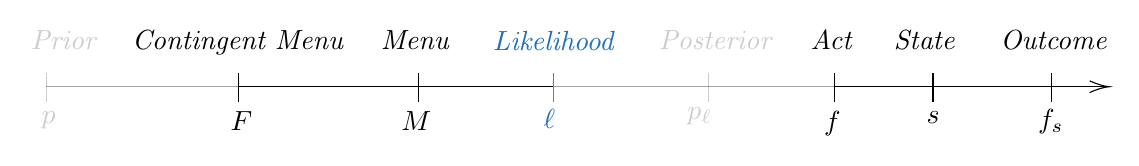
\begin{tikzpicture}[x=0.65pt,y=0.65pt,yscale=-1,xscale=1]
		% Uncomment if required: \path (0,472); % Set diagram left start at 0, and has height of 472

		% Draw the transparent horizontal line (arrow)
		\draw[opacity=0.2] (23,250) -- (614,250);

		% Draw the part of the horizontal arrow to the left of the vertical segment in transparent
		\draw[opacity=0.2] (23,250) -- (582,250);

		% Draw the part of the horizontal arrow to the right of the vertical segment in black
		\draw[black] (130,250) -- (305,250);
		\draw[black] (461,250) -- (614,250);

		% Draw the black oblique segments at the end of the horizontal arrow (pointing left)
		\draw[black, shift={(614,250)}, rotate=180]
		(10.93,-3.29) .. controls (6.95,-1.4) and (3.31,-0.3) .. (0,0) .. controls (3.31,0.3) and (6.95,1.4) .. (10.93,3.29);

		% Draw the small vertical segments below each word
		\draw[opacity=0.2] (23,242.5) -- (23,258.5);
		\draw[opacity=0.2] (130,242.5) -- (130,258.5);
		\draw[opacity=0.2] (230,242.5) -- (230,258.5);
		\draw[opacity=0.2] (305,242.5) -- (305,258.5);
		\draw[opacity=0.2] (391,242.5) -- (391,258.5);

		% The vertical segment below "Outcome, State, Act, Menu, Contingent Menu" in black
		\draw[black] (582,242.5) -- (582,258.5);
		\draw[black] (516,242.5) -- (516,258.5);
		\draw[black] (461,242.5) -- (461,258.5);
		\draw[black] (230,242.5) -- (230,258.5);
		\draw[black] (130,242.5) -- (130,258.5);

		% The word "Outcome, State, Act, Menu, Contingent Menu" in black
		\draw[opacity=1, black] (552,217.5) node [anchor=north west][inner sep=0.75pt] [align=left] {\textit{Outcome}};
		\draw[opacity=1, black] (492.74,217.5) node [anchor=north west][inner sep=0.75pt] [align=left] {\textit{State}};
		\draw[opacity=1, black] (446.45,217.5) node [anchor=north west][inner sep=0.75pt] [align=left] {\textit{Act}};
		\draw[opacity=1, black] (207.58,217.5) node [anchor=north west][inner sep=0.75pt] [align=left] {\textit{Menu}};
		\draw[opacity=1, black] (69.29,217.5) node [anchor=north west][inner sep=0.75pt] [align=left] {\textit{Contingent Menu}};

		% The vertical segment below "Likelihood" in RoyalBlue
		\draw[opacity=1, RoyalBlue] (305,242.5) -- (305,258.5);

		% The word "Likelihood" in RoyalBlue
		\draw[opacity=1, RoyalBlue] (269.87,217.5) node [anchor=north west][inner sep=0.75pt] [align=left] {\textit{Likelihood}};

		% The symbol "s, f_s, f, M, F" in black
		\draw[opacity=1, black] (511,262.15) node [anchor=north west][inner sep=0.75pt] {\(s\)};
		\draw[opacity=1, black] (573,261.15) node [anchor=north west][inner sep=0.75pt] {\(f_{s}\)};
		\draw[opacity=1, black] (454,262.15) node [anchor=north west][inner sep=0.75pt] {\(f\)};
		\draw[opacity=1, black] (219,262.15) node [anchor=north west][inner sep=0.75pt] {\(M\)};
		\draw[opacity=1, black] (124,262.15) node [anchor=north west][inner sep=0.75pt] {\( F \)};

		% The symbol "\ell_m,f" in RoyalBlue
		\draw[opacity=1, RoyalBlue] (298,261.15) node [anchor=north west][inner sep=0.75pt] {\(\ell\)};

		% Text for symbols (bottom) with reduced opacity
		\draw[opacity=0.2] (378,260.15) node [anchor=north west][inner sep=0.75pt] {\(p_{\ell}\)};
		\draw[opacity=0.2] (298,261.15) node [anchor=north west][inner sep=0.75pt] {\(\ell\)};
		\draw[opacity=0.2] (19,262.15) node [anchor=north west][inner sep=0.75pt] {\(p\)};

		% Text for labels (top) with reduced opacity
		\draw[opacity=0.2] (362.16,217.5) node [anchor=north west][inner sep=0.75pt] [align=left] {\textit{Posterior}};
		\draw[opacity=0.2] (269.87,217.5) node [anchor=north west][inner sep=0.75pt] [align=left] {\textit{Likelihood}};
		\draw[opacity=0.2] (13,217.5) node [anchor=north west][inner sep=0.75pt] [align=left] {\textit{Prior}};
	\end{tikzpicture}

	\vfill

	\begin{columns}
		% Left Column (adjusted width)
		\begin{column}{0.35\textwidth} % Reduced width to make room for the right column
			\begin{center}
				\begin{table}
					\centering
					\begin{tikzpicture}[x=0.75pt,y=0.75pt,yscale=-1,xscale=1]
						%uncomment if require: \path (0,300); %set diagram left start at 0, and has height of 300

						%Straight Lines [id:da10589365900996173] 
						\draw [color={rgb, 255:red, 0; green, 0; blue, 0 }  ,draw opacity=1 ]   (262.33,132.1) -- (369.63,92.41) ;
						%Straight Lines [id:da5796893993758667] 
						\draw [color={rgb, 255:red, 0; green, 0; blue, 0 }  ,draw opacity=1 ]   (262.33,132.1) -- (369.63,171.91) ;
						%Straight Lines [id:da024405781766148493] 
						\draw [color={rgb, 255:red, 0; green, 0; blue, 0 }  ,draw opacity=1 ]   (262.33,132.1) -- (369.63,132.41) ;
						%Straight Lines [id:da569061638772357] 
						\draw  [dash pattern={on 0.84pt off 2.51pt}]  (372,94.78) -- (372,130.03) ;
						%Shape: Circle [id:dp5199064102665634] 
						\draw   (369.63,92.41) .. controls (369.63,91.09) and (370.69,90.03) .. (372,90.03) .. controls (373.31,90.03) and (374.38,91.09) .. (374.38,92.41) .. controls (374.38,93.72) and (373.31,94.78) .. (372,94.78) .. controls (370.69,94.78) and (369.63,93.72) .. (369.63,92.41) -- cycle ;
						%Shape: Circle [id:dp7343244546600616] 
						\draw   (369.63,132.41) .. controls (369.63,131.09) and (370.69,130.03) .. (372,130.03) .. controls (373.31,130.03) and (374.38,131.09) .. (374.38,132.41) .. controls (374.38,133.72) and (373.31,134.78) .. (372,134.78) .. controls (370.69,134.78) and (369.63,133.72) .. (369.63,132.41) -- cycle ;
						%Shape: Circle [id:dp8289076341983612] 
						\draw   (369.63,171.91) .. controls (369.63,170.59) and (370.69,169.53) .. (372,169.53) .. controls (373.31,169.53) and (374.38,170.59) .. (374.38,171.91) .. controls (374.38,173.22) and (373.31,174.28) .. (372,174.28) .. controls (370.69,174.28) and (369.63,173.22) .. (369.63,171.91) -- cycle ;

						% Text Node
						\draw (280.54,107.19) node [anchor=north west][inner sep=0.75pt]  [color={rgb, 255:red, 0; green, 0; blue, 0 }  ,opacity=1 ,rotate=-339.07]  {$Good$};
						% Text Node
						\draw (317.98,135.65) node [anchor=north west][inner sep=0.75pt]  [font=\small,color={rgb, 255:red, 0; green, 0; blue, 0 }  ,opacity=1 ]  {$Normal$};
						% Text Node
						\draw (214.83,123.7) node [anchor=north west][inner sep=0.75pt]    {$Check$};
						% Text Node
						\draw (297.77,148.06) node [anchor=north west][inner sep=0.75pt]  [color={rgb, 255:red, 0; green, 0; blue, 0 }  ,opacity=1 ,rotate=-19.16]  {$Bad$};
						% Text Node
						\draw (375.33,150.4) node [anchor=north west][inner sep=0.75pt]  [color=Black ,opacity=1 ]  {$1 \cdot \overset{\underline{p}}{\{i ,n\}}$};
						% Text Node
						\draw (375.75,95.4) node [anchor=north west][inner sep=0.75pt]  [color=Black ,opacity=1 ]  {$1 \cdot \overset{\overline{p}}{\{i ,n\}}$};
					\end{tikzpicture}
				\end{table}
			\end{center}
		\end{column}

		% Right Column (adjusted width to take up more space)
		\begin{column}{0.55\textwidth} % Increased width to make room for the content
			\begin{itemize}
				\item a contingent menu is \(F: States \: \rightarrow \: Menus \);
				\item probability \( M \) realises in state \( s \) is \( F_s \left( M \right) \);
			\end{itemize}
		\end{column}
	\end{columns}

	\vspace{0.6cm}

	The normalised likelihood of state \(Good\) after realisation of menu \( \overset{\overline{p}}{\{i ,n\}} \) is

	\vfill

	\[ \ell \left( Good \right) = \frac{1}{1+1} = \frac{1}{2} .
	\]

\end{frame}

\begin{frame}[noframenumbering]{Model: Information}

	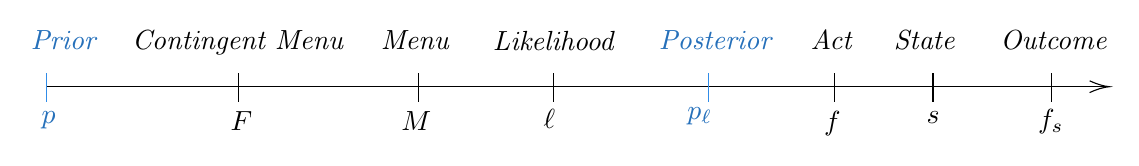
\begin{tikzpicture}[x=0.65pt,y=0.65pt,yscale=-1,xscale=1]
		% Uncomment if required: \path (0,472); % Set diagram left start at 0, and has height of 472

		% Draw the transparent horizontal line (arrow)
		\draw[opacity=0.2] (23,250) -- (614,250);

		% Draw the part of the horizontal arrow to the left of the vertical segment in transparent
		\draw[opacity=0.2] (23,250) -- (582,250);

		% Draw the part of the horizontal arrow to the right of the vertical segment in black
		\draw[black] (23,250) -- (461,250);
		\draw[black] (461,250) -- (614,250);

		% Draw the black oblique segments at the end of the horizontal arrow (pointing left)
		\draw[black, shift={(614,250)}, rotate=180]
		(10.93,-3.29) .. controls (6.95,-1.4) and (3.31,-0.3) .. (0,0) .. controls (3.31,0.3) and (6.95,1.4) .. (10.93,3.29);

		% Draw the small vertical segments below each word
		\draw[opacity=0.2] (23,242.5) -- (23,258.5);
		\draw[opacity=0.2] (130,242.5) -- (130,258.5);
		\draw[opacity=0.2] (230,242.5) -- (230,258.5);
		\draw[opacity=0.2] (305,242.5) -- (305,258.5);
		\draw[opacity=0.2] (391,242.5) -- (391,258.5);

		% The vertical segment below "Outcome, State, Act, Menu, Contingent Menu, Likelihood" in black
		\draw[black] (582,242.5) -- (582,258.5);
		\draw[black] (516,242.5) -- (516,258.5);
		\draw[black] (461,242.5) -- (461,258.5);
		\draw[black] (230,242.5) -- (230,258.5);
		\draw[black] (130,242.5) -- (130,258.5);
		\draw[black] (305,242.5) -- (305,258.5);

		% The word "Outcome, State, Act, Menu, Contingent Menu, Likelihood" in black
		\draw[opacity=1, black] (552,217.5) node [anchor=north west][inner sep=0.75pt] [align=left] {\textit{Outcome}};
		\draw[opacity=1, black] (492.74,217.5) node [anchor=north west][inner sep=0.75pt] [align=left] {\textit{State}};
		\draw[opacity=1, black] (446.45,217.5) node [anchor=north west][inner sep=0.75pt] [align=left] {\textit{Act}};
		\draw[opacity=1, black] (207.58,217.5) node [anchor=north west][inner sep=0.75pt] [align=left] {\textit{Menu}};
		\draw[opacity=1, black] (69.29,217.5) node [anchor=north west][inner sep=0.75pt] [align=left] {\textit{Contingent Menu}};
		\draw[opacity=1, black] (269.87,217.5) node [anchor=north west][inner sep=0.75pt] [align=left] {\textit{Likelihood}};

		% The vertical segment below "Prior, Posterior" in RoyalBlue
		\draw[opacity=1, RoyalBlue] (23,242.5) -- (23,258.5);
		\draw[opacity=1, RoyalBlue] (391,242.5) -- (391,258.5);

		% The word "Prior, Posterior" in RoyalBlue
		\draw[opacity=1, RoyalBlue] (362.16,217.5) node [anchor=north west][inner sep=0.75pt] [align=left] {\textit{Posterior}};
		\draw[opacity=1, RoyalBlue] (13,217.5) node [anchor=north west][inner sep=0.75pt] [align=left] {\textit{Prior}};

		% The symbol "s, f_s, f, M, F, \ell_m,f" in black
		\draw[opacity=1, black] (511,262.15) node [anchor=north west][inner sep=0.75pt] {\(s\)};
		\draw[opacity=1, black] (573,261.15) node [anchor=north west][inner sep=0.75pt] {\(f_{s}\)};
		\draw[opacity=1, black] (454,262.15) node [anchor=north west][inner sep=0.75pt] {\(f\)};
		\draw[opacity=1, black] (219,262.15) node [anchor=north west][inner sep=0.75pt] {\(M\)};
		\draw[opacity=1, black] (124,262.15) node [anchor=north west][inner sep=0.75pt] {\( F \)};
		\draw[opacity=1, black] (298,261.15) node [anchor=north west][inner sep=0.75pt] {\(\ell\)};

		% The symbol "p, p_\ell" in RoyalBlue
		\draw[opacity=1, RoyalBlue] (378,260.15) node [anchor=north west][inner sep=0.75pt] {\(p_{\ell}\)};
		\draw[opacity=1, RoyalBlue] (19,262.15) node [anchor=north west][inner sep=0.75pt] {\(p\)};

		% Text for symbols (bottom) with reduced opacity
		\draw[opacity=0.2] (378,260.15) node [anchor=north west][inner sep=0.75pt] {\(p_{\ell}\)};
		\draw[opacity=0.2] (19,262.15) node [anchor=north west][inner sep=0.75pt] {\(p\)};

		% Text for labels (top) with reduced opacity
		\draw[opacity=0.2] (362.16,217.5) node [anchor=north west][inner sep=0.75pt] [align=left] {\textit{Posterior}};
		\draw[opacity=0.2] (13,217.5) node [anchor=north west][inner sep=0.75pt] [align=left] {\textit{Prior}};
	\end{tikzpicture}

	\vfill

	\begin{columns}
		% Left Column (adjusted width)
		\begin{column}{0.35\textwidth} % Reduced width to make room for the right column
			\begin{center}
				\begin{table}
					\centering
					\begin{tikzpicture}[x=0.75pt,y=0.75pt,yscale=-1,xscale=1]
						%uncomment if require: \path (0,300); %set diagram left start at 0, and has height of 300

						%Straight Lines [id:da10589365900996173] 
						\draw [color={rgb, 255:red, 0; green, 0; blue, 0 }  ,draw opacity=1 ]   (262.33,132.1) -- (369.63,92.41) ;
						%Straight Lines [id:da5796893993758667] 
						\draw [color={rgb, 255:red, 0; green, 0; blue, 0 }  ,draw opacity=1 ]   (262.33,132.1) -- (369.63,171.91) ;
						%Straight Lines [id:da024405781766148493] 
						\draw [color={rgb, 255:red, 0; green, 0; blue, 0 }  ,draw opacity=1 ]   (262.33,132.1) -- (369.63,132.41) ;
						%Straight Lines [id:da569061638772357] 
						\draw  [dash pattern={on 0.84pt off 2.51pt}]  (372,94.78) -- (372,130.03) ;
						%Shape: Circle [id:dp5199064102665634] 
						\draw   (369.63,92.41) .. controls (369.63,91.09) and (370.69,90.03) .. (372,90.03) .. controls (373.31,90.03) and (374.38,91.09) .. (374.38,92.41) .. controls (374.38,93.72) and (373.31,94.78) .. (372,94.78) .. controls (370.69,94.78) and (369.63,93.72) .. (369.63,92.41) -- cycle ;
						%Shape: Circle [id:dp7343244546600616] 
						\draw   (369.63,132.41) .. controls (369.63,131.09) and (370.69,130.03) .. (372,130.03) .. controls (373.31,130.03) and (374.38,131.09) .. (374.38,132.41) .. controls (374.38,133.72) and (373.31,134.78) .. (372,134.78) .. controls (370.69,134.78) and (369.63,133.72) .. (369.63,132.41) -- cycle ;
						%Shape: Circle [id:dp8289076341983612] 
						\draw   (369.63,171.91) .. controls (369.63,170.59) and (370.69,169.53) .. (372,169.53) .. controls (373.31,169.53) and (374.38,170.59) .. (374.38,171.91) .. controls (374.38,173.22) and (373.31,174.28) .. (372,174.28) .. controls (370.69,174.28) and (369.63,173.22) .. (369.63,171.91) -- cycle ;

						% Text Node
						\draw (280.54,107.19) node [anchor=north west][inner sep=0.75pt]  [color={rgb, 255:red, 0; green, 0; blue, 0 }  ,opacity=1 ,rotate=-339.07]  {$Good$};
						% Text Node
						\draw (317.98,135.65) node [anchor=north west][inner sep=0.75pt]  [font=\small,color={rgb, 255:red, 0; green, 0; blue, 0 }  ,opacity=1 ]  {$Normal$};
						% Text Node
						\draw (214.83,123.7) node [anchor=north west][inner sep=0.75pt]    {$Check$};
						% Text Node
						\draw (297.77,148.06) node [anchor=north west][inner sep=0.75pt]  [color={rgb, 255:red, 0; green, 0; blue, 0 }  ,opacity=1 ,rotate=-19.16]  {$Bad$};
						% Text Node
						\draw (375.33,150.4) node [anchor=north west][inner sep=0.75pt]  [color=Black ,opacity=1 ]  {$1 \cdot \overset{\underline{p}}{\{i ,n\}}$};
						% Text Node
						\draw (375.75,95.4) node [anchor=north west][inner sep=0.75pt]  [color=Black ,opacity=1 ]  {$1 \cdot \overset{\overline{p}}{\{i ,n\}}$};
					\end{tikzpicture}
				\end{table}
			\end{center}
		\end{column}

		% Right Column (adjusted width to take up more space)
		\begin{column}{0.6\textwidth} % Increased width to make room for the content
			\begin{itemize}
				\item a contingent menu is \(F: States \: \rightarrow \: Menus \);
				\item probability \( M \) realises in state \( s \) is \( F_s \left( M \right) \);
				\item prior \( \textcolor{RoyalBlue}{p} \) and likelihood \( \ell \) induce posterior \( \textcolor{RoyalBlue}{p_{\ell}} \).
			\end{itemize}
		\end{column}
	\end{columns}

	\vspace{0.6cm}

	The likelihood of state \(s\) after realisation of menu \(M\) from the contingent menu \(F\) is

	\vfill

	\[ \ell_{M, F} \left( s \right) = \frac{F_{s} \left( M \right)}{ \sum_{s^{\prime} \in S} F_{s^{\prime}} \left( M \right)} .
	\]

\end{frame}

\begin{frame}{Utility over acts}


	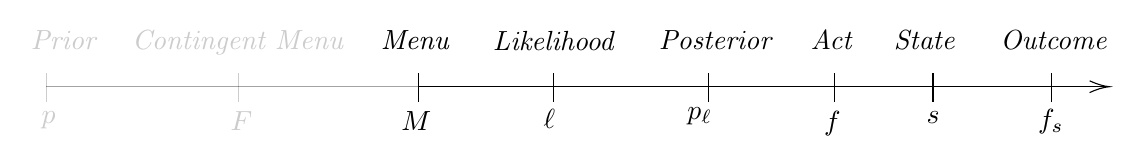
\begin{tikzpicture}[x=0.65pt,y=0.65pt,yscale=-1,xscale=1]
		% Uncomment if required: \path (0,472); % Set diagram left start at 0, and has height of 472

		% Draw the transparent horizontal line (arrow)
		\draw[opacity=0.2] (23,250) -- (614,250);

		% Draw the part of the horizontal arrow to the left of the vertical segment in transparent
		\draw[opacity=0.2] (23,250) -- (582,250);

		% Draw the part of the horizontal arrow to the right of the vertical segment in black
		\draw[black] (230,250) -- (614,250);

		% Draw the black oblique segments at the end of the horizontal arrow (pointing left)
		\draw[black, shift={(614,250)}, rotate=180]
		(10.93,-3.29) .. controls (6.95,-1.4) and (3.31,-0.3) .. (0,0) .. controls (3.31,0.3) and (6.95,1.4) .. (10.93,3.29);

		% Draw the small vertical segments below each word
		\draw[opacity=0.2] (23,242.5) -- (23,258.5);
		\draw[opacity=0.2] (130,242.5) -- (130,258.5);
		\draw[opacity=0.2] (230,242.5) -- (230,258.5);
		\draw[black] (305,242.5) -- (305,258.5);
		\draw[black] (391,242.5) -- (391,258.5);

		% The vertical segment below "Outcome, State, Act" in black
		\draw[black] (582,242.5) -- (582,258.5);
		\draw[black] (516,242.5) -- (516,258.5);
		\draw[black] (461,242.5) -- (461,258.5);

		% The word "Outcome, State, Act" in black
		\draw[opacity=1, black] (552,217.5) node [anchor=north west][inner sep=0.75pt] [align=left] {\textit{Outcome}};
		\draw[opacity=1, black] (492.74,217.5) node [anchor=north west][inner sep=0.75pt] [align=left] {\textit{State}};
		\draw[opacity=1, black] (446.45,217.5) node [anchor=north west][inner sep=0.75pt] [align=left] {\textit{Act}};

		% The vertical segment below "Menu" in RoyalBlue
		\draw[opacity=1, black] (230,242.5) -- (230,258.5);

		% The word "Menu" in RoyalBlue
		\draw[opacity=1, black] (207.58,217.5) node [anchor=north west][inner sep=0.75pt] [align=left] {\textit{Menu}};

		% The symbol "s, f_s, f" in black
		\draw[opacity=1, black] (511,262.15) node [anchor=north west][inner sep=0.75pt] {\(s\)};
		\draw[opacity=1, black] (573,261.15) node [anchor=north west][inner sep=0.75pt] {\(f_{s}\)};
		\draw[opacity=1, black] (454,262.15) node [anchor=north west][inner sep=0.75pt] {\(f\)};

		% The symbol "M" in RoyalBlue
		\draw[opacity=1, black] (219,262.15) node [anchor=north west][inner sep=0.75pt] {\(M\)};

		% Text for symbols (bottom) with reduced opacity
		\draw[opacity=0.2] (124,262.15) node [anchor=north west][inner sep=0.75pt] {\( F \)};
		\draw[opacity=0.2] (219,262.15) node [anchor=north west][inner sep=0.75pt] {\(M\)};
		\draw[opacity=1, black] (378,260.15) node [anchor=north west][inner sep=0.75pt] {\(p_{\ell}\)};
		\draw[opacity=0.2] (573,261.15) node [anchor=north west][inner sep=0.75pt] {\(f_{s}\)};
		\draw[opacity=0.2] (454,262.15) node [anchor=north west][inner sep=0.75pt] {\(f\)};
		\draw[opacity=1, black] (298,261.15) node [anchor=north west][inner sep=0.75pt] {\(\ell\)};
		\draw[opacity=0.2] (19,262.15) node [anchor=north west][inner sep=0.75pt] {\(p\)};

		% Text for labels (top) with reduced opacity
		\draw[opacity=0.2] (69.29,217.5) node [anchor=north west][inner sep=0.75pt] [align=left] {\textit{Contingent Menu}};
		\draw[opacity=0.2] (207.58,217.5) node [anchor=north west][inner sep=0.75pt] [align=left] {\textit{Menu}};
		\draw[opacity=1, black] (362.16,217.5) node [anchor=north west][inner sep=0.75pt] [align=left] {\textit{Posterior}};
		\draw[opacity=1, black] (269.87,217.5) node [anchor=north west][inner sep=0.75pt] [align=left] {\textit{Likelihood}};
		\draw[opacity=0.2] (13,217.5) node [anchor=north west][inner sep=0.75pt] [align=left] {\textit{Prior}};
	\end{tikzpicture}

	\vspace{0.2cm}

	\begin{center}  % Center the columns in the overall slide
		\begin{columns}
			% Left Column (adjusted width and smaller table font)
			\begin{column}{0.5\textwidth}
				Expected utility of act \( f \) at likelihood \( \textcolor{RoyalBlue}{\ell} \)
				\vfill
				\[
					\sum_{s} p_{\textcolor{RoyalBlue}{\ell}} \left( s \right) u \left( f_{s} ; \textcolor{RoyalBlue}{\ell} \right) .
				\]
				\pause
			\end{column}

			% Right Column (slightly reduced width)
			\begin{column}{0.5\textwidth}
				Individual distorts the likelihood to \( \textcolor{red}{\ell^{*}} \)
				\vfill
				\[
					\sum_{s} p_{\textcolor{red}{\ell^{*}}} \left( s \right) u \left( f_{s} ; \textcolor{red}{\ell^{*}} \right).
				\]
				\pause
			\end{column}
		\end{columns}
	\end{center}

	\vfill

	The main theorem identifies conditions under which the individual solves

	\vfill

	\[
		\max _{f \in M} \left\{ \underbrace{\sum_{s} p_{\textcolor{RoyalBlue}{\ell}}(s) u \left( f_{s}; \textcolor{RoyalBlue}{\ell} \right)}_{\text{\textit{\textcolor{RoyalBlue}{EU}}}} +
		\alpha_{\ell} \underbrace{\sum_{s} p_{\textcolor{red}{\ell^{*}}} \left( s \right) u \left( f_{s} ; \textcolor{red}{\ell^{*}} \right)}_{\text{\textit{\textcolor{red}{distorted EU}}}} \right\} .
	\]

\end{frame}

\begin{frame}[noframenumbering]{Utility over acts}


	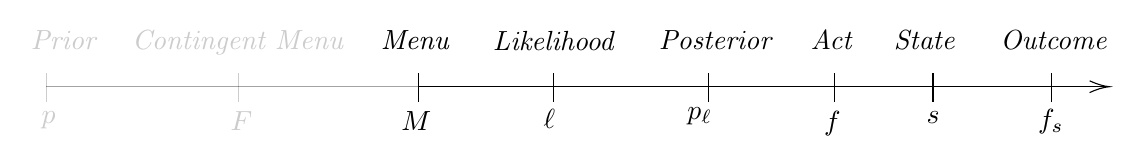
\begin{tikzpicture}[x=0.65pt,y=0.65pt,yscale=-1,xscale=1]
		% Uncomment if required: \path (0,472); % Set diagram left start at 0, and has height of 472

		% Draw the transparent horizontal line (arrow)
		\draw[opacity=0.2] (23,250) -- (614,250);

		% Draw the part of the horizontal arrow to the left of the vertical segment in transparent
		\draw[opacity=0.2] (23,250) -- (582,250);

		% Draw the part of the horizontal arrow to the right of the vertical segment in black
		\draw[black] (230,250) -- (614,250);

		% Draw the black oblique segments at the end of the horizontal arrow (pointing left)
		\draw[black, shift={(614,250)}, rotate=180]
		(10.93,-3.29) .. controls (6.95,-1.4) and (3.31,-0.3) .. (0,0) .. controls (3.31,0.3) and (6.95,1.4) .. (10.93,3.29);

		% Draw the small vertical segments below each word
		\draw[opacity=0.2] (23,242.5) -- (23,258.5);
		\draw[opacity=0.2] (130,242.5) -- (130,258.5);
		\draw[opacity=0.2] (230,242.5) -- (230,258.5);
		\draw[black] (305,242.5) -- (305,258.5);
		\draw[black] (391,242.5) -- (391,258.5);

		% The vertical segment below "Outcome, State, Act" in black
		\draw[black] (582,242.5) -- (582,258.5);
		\draw[black] (516,242.5) -- (516,258.5);
		\draw[black] (461,242.5) -- (461,258.5);

		% The word "Outcome, State, Act" in black
		\draw[opacity=1, black] (552,217.5) node [anchor=north west][inner sep=0.75pt] [align=left] {\textit{Outcome}};
		\draw[opacity=1, black] (492.74,217.5) node [anchor=north west][inner sep=0.75pt] [align=left] {\textit{State}};
		\draw[opacity=1, black] (446.45,217.5) node [anchor=north west][inner sep=0.75pt] [align=left] {\textit{Act}};

		% The vertical segment below "Menu" in RoyalBlue
		\draw[opacity=1, black] (230,242.5) -- (230,258.5);

		% The word "Menu" in RoyalBlue
		\draw[opacity=1, black] (207.58,217.5) node [anchor=north west][inner sep=0.75pt] [align=left] {\textit{Menu}};

		% The symbol "s, f_s, f" in black
		\draw[opacity=1, black] (511,262.15) node [anchor=north west][inner sep=0.75pt] {\(s\)};
		\draw[opacity=1, black] (573,261.15) node [anchor=north west][inner sep=0.75pt] {\(f_{s}\)};
		\draw[opacity=1, black] (454,262.15) node [anchor=north west][inner sep=0.75pt] {\(f\)};

		% The symbol "M" in RoyalBlue
		\draw[opacity=1, black] (219,262.15) node [anchor=north west][inner sep=0.75pt] {\(M\)};

		% Text for symbols (bottom) with reduced opacity
		\draw[opacity=0.2] (124,262.15) node [anchor=north west][inner sep=0.75pt] {\( F \)};
		\draw[opacity=0.2] (219,262.15) node [anchor=north west][inner sep=0.75pt] {\(M\)};
		\draw[opacity=1, black] (378,260.15) node [anchor=north west][inner sep=0.75pt] {\(p_{\ell}\)};
		\draw[opacity=0.2] (573,261.15) node [anchor=north west][inner sep=0.75pt] {\(f_{s}\)};
		\draw[opacity=0.2] (454,262.15) node [anchor=north west][inner sep=0.75pt] {\(f\)};
		\draw[opacity=1, black] (298,261.15) node [anchor=north west][inner sep=0.75pt] {\(\ell\)};
		\draw[opacity=0.2] (19,262.15) node [anchor=north west][inner sep=0.75pt] {\(p\)};

		% Text for labels (top) with reduced opacity
		\draw[opacity=0.2] (69.29,217.5) node [anchor=north west][inner sep=0.75pt] [align=left] {\textit{Contingent Menu}};
		\draw[opacity=0.2] (207.58,217.5) node [anchor=north west][inner sep=0.75pt] [align=left] {\textit{Menu}};
		\draw[opacity=1, black] (362.16,217.5) node [anchor=north west][inner sep=0.75pt] [align=left] {\textit{Posterior}};
		\draw[opacity=1, black] (269.87,217.5) node [anchor=north west][inner sep=0.75pt] [align=left] {\textit{Likelihood}};
		\draw[opacity=0.2] (13,217.5) node [anchor=north west][inner sep=0.75pt] [align=left] {\textit{Prior}};
	\end{tikzpicture}

	\vspace{0.2cm}

	\begin{center}  % Center the columns in the overall slide
		\begin{columns}
			% Left Column (adjusted width and smaller table font)
			\begin{column}{0.5\textwidth}
				Expected utility of act \( f \) at likelihood \( \textcolor{RoyalBlue}{\ell} \)
				\vfill
				\[
					\sum_{s} p_{\textcolor{RoyalBlue}{\ell}} \left( s \right) u \left( f_{s} ; \textcolor{RoyalBlue}{p_{\ell}} \right) .
				\]
			\end{column}

			% Right Column (slightly reduced width)
			\begin{column}{0.5\textwidth}
				Individual distorts the likelihood to \( \textcolor{red}{\ell^{*}} \)
				\vfill
				\[
					\sum_{s} p_{\textcolor{red}{\ell^{*}}} \left( s \right) u \left( f_{s} ; \textcolor{red}{p_{\ell^{*}}} \right).
				\]
			\end{column}
		\end{columns}
	\end{center}

	\vfill

	The main theorem identifies conditions under which the individual solves

	\vfill

	\[
		\max _{f \in M} \left\{ \underbrace{\sum_{s} p_{\textcolor{RoyalBlue}{\ell}}(s) u \left( f_{s}; \textcolor{RoyalBlue}{p_{\ell}} \right)}_{\text{\textit{\textcolor{RoyalBlue}{EU}}}} +
		\alpha_{\ell} \underbrace{\sum_{s} p_{\textcolor{red}{\ell^{*}}} \left( s \right) u \left( f_{s} ; \textcolor{red}{p_{\ell^{*}}} \right)}_{\text{\textit{\textcolor{red}{distorted EU}}}} \right\} .
	\]

\end{frame}

\begin{frame}{Utility over contingent menus}\label{fullmodel}

	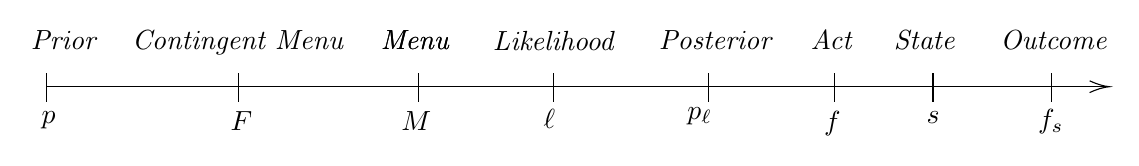
\begin{tikzpicture}[x=0.65pt,y=0.65pt,yscale=-1,xscale=1]
		% Uncomment if required: \path (0,472); % Set diagram left start at 0, and has height of 472

		% Draw the black horizontal line (arrow)
		\draw[opacity=1] (23,250) -- (614,250);

		% Draw the part of the horizontal arrow to the left of the vertical segment in black
		\draw[opacity=1] (23,250) -- (582,250);

		% Draw the part of the horizontal arrow to the right of the vertical segment in black
		\draw[opacity=1] (230,250) -- (614,250);

		% Draw the black oblique segments at the end of the horizontal arrow (pointing left)
		\draw[opacity=1, shift={(614,250)}, rotate=180]
		(10.93,-3.29) .. controls (6.95,-1.4) and (3.31,-0.3) .. (0,0) .. controls (3.31,0.3) and (6.95,1.4) .. (10.93,3.29);

		% Draw the small vertical segments below each word in black
		\draw[opacity=1] (23,242.5) -- (23,258.5);
		\draw[opacity=1] (130,242.5) -- (130,258.5);
		\draw[opacity=1] (230,242.5) -- (230,258.5);
		\draw[opacity=1] (305,242.5) -- (305,258.5);
		\draw[opacity=1] (391,242.5) -- (391,258.5);
		\draw[opacity=1] (461,242.5) -- (461,258.5);
		\draw[opacity=1] (516,242.5) -- (516,258.5);

		% The vertical segment below "Outcome, State, Act" in black
		\draw[opacity=1] (582,242.5) -- (582,258.5);
		\draw[opacity=1] (516,242.5) -- (516,258.5);
		\draw[opacity=1] (461,242.5) -- (461,258.5);

		% The words "Outcome, State, Act" in black
		\draw[opacity=1] (552,217.5) node [anchor=north west][inner sep=0.75pt] [align=left] {\textit{Outcome}};
		\draw[opacity=1] (492.74,217.5) node [anchor=north west][inner sep=0.75pt] [align=left] {\textit{State}};
		\draw[opacity=1] (446.45,217.5) node [anchor=north west][inner sep=0.75pt] [align=left] {\textit{Act}};

		% The vertical segment below "Menu" in black
		\draw[opacity=1] (230,242.5) -- (230,258.5);

		% The word "Menu" in black
		\draw[opacity=1] (207.58,217.5) node [anchor=north west][inner sep=0.75pt] [align=left] {\textit{Menu}};

		% The symbols "s, f_s, f" in black
		\draw[opacity=1] (511,262.15) node [anchor=north west][inner sep=0.75pt] {\(s\)};
		\draw[opacity=1] (573,261.15) node [anchor=north west][inner sep=0.75pt] {\(f_{s}\)};
		\draw[opacity=1] (454,262.15) node [anchor=north west][inner sep=0.75pt] {\(f\)};

		% The symbol "M" in black
		\draw[opacity=1] (219,262.15) node [anchor=north west][inner sep=0.75pt] {\(M\)};

		% Text for symbols (bottom) with black opacity
		\draw[opacity=1] (124,262.15) node [anchor=north west][inner sep=0.75pt] {\( F \)};
		\draw[opacity=1] (378,260.15) node [anchor=north west][inner sep=0.75pt] {\(p_{\ell}\)};
		\draw[opacity=1] (298,261.15) node [anchor=north west][inner sep=0.75pt] {\(\ell\)};
		\draw[opacity=1] (19,262.15) node [anchor=north west][inner sep=0.75pt] {\(p\)};

		% Text for labels (top) in black
		\draw[opacity=1] (69.29,217.5) node [anchor=north west][inner sep=0.75pt] [align=left] {\textit{Contingent Menu}};
		\draw[opacity=1] (207.58,217.5) node [anchor=north west][inner sep=0.75pt] [align=left] {\textit{Menu}};
		\draw[opacity=1] (362.16,217.5) node [anchor=north west][inner sep=0.75pt] [align=left] {\textit{Posterior}};
		\draw[opacity=1] (269.87,217.5) node [anchor=north west][inner sep=0.75pt] [align=left] {\textit{Likelihood}};
		\draw[opacity=1] (13,217.5) node [anchor=north west][inner sep=0.75pt] [align=left] {\textit{Prior}};
	\end{tikzpicture}

	\vspace{0.55cm}

	The individual anticipates her choices and cost of temptation

	\vfill

	\[
		\begin{aligned}
			\mathcal{U} \left(M ; \ell \right) = \max _{\textcolor{RoyalBlue}{f} \in M}\left\{\sum_{s} p_{\ell} \left( s \right) u \left( f_{s} ; \ell \right) + \right. & \left. \alpha_{\ell} \sum_{s} p_{\ell^{*}} \left( s \right) u \left( \textcolor{RoyalBlue}{f_{s}} ; \ell^{*} \right) \right\} \\
			-\max _{\textcolor{red}{f^{\prime}} \in M}                                                                                                                   & \: \alpha _{\ell} \sum_{s} p_{\ell^{*}} \left( s \right) u\left(\textcolor{red}{f^{\prime}_{s}} ; \ell^{*} \right) .
		\end{aligned}
	\]

	\vfill

	The positive number \( \alpha_{\ell} \) captures the \textit{strength of motivated reasoning}.  \: \: \hyperlink{alpha}{\beamerbutton{Alpha?}} \: \: \hyperlink{cost}{\beamerbutton{Cost?}}

\end{frame}

\begin{frame}[noframenumbering]{Utility over contingent menus}


	\[
		\begin{aligned}
			\mathcal{U} \left(M ; \ell \right) = \max _{f \in M}\left\{\sum_{s} p_{\ell} \left( s \right) u \left( f_{s} ; \ell \right) + \right. & \left. \alpha_{\ell} \sum_{s} p_{\ell^{*}} \left( s \right) u \left( f_{s} ; \ell^{*} \right) \right\} \\
			-\max _{f^{\prime} \in M}                                                                                                             & \: \alpha _{\ell} \sum_{s} p_{\ell^{*}} \left( s \right) u\left(f^{\prime}_{s} ; \ell^{*} \right) .
		\end{aligned}
	\]

	Expected utility of contingent menu \( \textcolor{RoyalBlue}{F} \) is

	\vfill
	\[
		\mathscr{U}(\textcolor{RoyalBlue}{F})= \sum_{M} \sum_{s} p \left( s \right) F_{s} \left( M \right) \mathcal{U} \left(M ; \ell_{M, F} \right) .
	\]

	\vfill

	Choices over \textcolor{RoyalBlue}{contingent menus} are sufficient for identification of \( u, p, \ell^{*}, \alpha_{\ell} \).

\end{frame}

\begin{frame}{Distorted likelihood}

	Each likelihood \( \ell \) is consistent with one even \( S_{\ell} \).

	\vfill

	\begin{center}
		\begin{tikzpicture}[x=0.75pt,y=0.75pt,yscale=-1,xscale=1]
			%uncomment if require: \path (0,341); %set diagram left start at 0, and has height of 341

			%Straight Lines [id:da6521689763503256] 
			\draw [color=RoyalBlue, draw opacity=1]   (259.33,139.1) -- (366.63,99.41) ;
			%Straight Lines [id:da3094065715046459] 
			\draw [color=Red, draw opacity=1]   (259.33,139.1) -- (366.63,178.91) ;
			%Straight Lines [id:da3636097363244992] 
			\draw [color=RoyalBlue, draw opacity=1]   (259.33,139.1) -- (366.63,139.41) ;
			%Straight Lines [id:da7301255340273027] 
			\draw  [dash pattern={on 0.84pt off 2.51pt}]  (369,99.41) -- (369,139.41) ;
			%Shape: Circle [id:dp5572573680385027] 
			\draw   (366.63,99.41) .. controls (366.63,98.09) and (367.69,97.03) .. (369,97.03) .. controls (370.31,97.03) and (371.38,98.09) .. (371.38,99.41) .. controls (371.38,100.72) and (370.31,101.78) .. (369,101.78) .. controls (367.69,101.78) and (366.63,100.72) .. (366.63,99.41) -- cycle ;
			%Shape: Circle [id:dp045414237311399264] 
			\draw   (366.63,139.41) .. controls (366.63,138.09) and (367.69,137.03) .. (369,137.03) .. controls (370.31,137.03) and (371.38,138.09) .. (371.38,139.41) .. controls (371.38,140.72) and (370.31,141.78) .. (369,141.78) .. controls (367.69,141.78) and (366.63,140.72) .. (366.63,139.41) -- cycle ;
			%Shape: Circle [id:dp6206756734194616] 
			\draw   (366.63,178.91) .. controls (366.63,177.59) and (367.69,176.53) .. (369,176.53) .. controls (370.31,176.53) and (371.38,177.59) .. (371.38,178.91) .. controls (371.38,180.22) and (370.31,181.28) .. (369,181.28) .. controls (367.69,181.28) and (366.63,180.22) .. (366.63,178.91) -- cycle ;

			% Text Node
			\draw (277.54,114.19) node [anchor=north west][inner sep=0.75pt]  [color=RoyalBlue ,opacity=1 ,rotate=-339.07]  {$Good$};
			% Text Node
			\draw (314.98,142.65) node [anchor=north west][inner sep=0.75pt]  [font=\small,color=RoyalBlue ,opacity=1 ]  {$Normal$};
			% Text Node
			\draw (211.83,130.7) node [anchor=north west][inner sep=0.75pt]    {$Check$};
			% Text Node
			\draw (294.77,155.06) node [anchor=north west][inner sep=0.75pt]  [color=Red ,opacity=1 ,rotate=-19.16]  {$Bad$};
			% Text Node
			\draw (371.33,156.4) node [anchor=north west][inner sep=0.75pt]  [color=Red ,opacity=1 ]  {$\overset{\underline{p}}{\{i ,n\}}$};
			% Text Node
			\draw (370.83,98.4) node [anchor=north west][inner sep=0.75pt]  [color=RoyalBlue ,opacity=1 ]  {$\overset{\overline{p}}{\{i ,n\}}$};

		\end{tikzpicture}
	\end{center} \pause

	\vfill

	The distorted likelihood \( \ell^{*}_{S} \) at event \( S \) is the best one according to \( u \):

	\vfill

	\[
		\ell^{*}_{S} \in \underset{\ell \in \Delta \left( S \right) }{\arg \max} \: u \left( x ; \ell \right)  \pause \hspace{0.3cm} \dots \hspace{0.3cm} \text{not well defined!}
	\]

\end{frame}

\begin{frame}[noframenumbering]{Distorted likelihood}\label{distortedlikelihood}

	Each likelihood \( \ell \) is consistent with one event \( S_{\ell} \).

	\vfill

	\begin{center}
		\begin{tikzpicture}[x=0.75pt,y=0.75pt,yscale=-1,xscale=1]
			%uncomment if require: \path (0,341); %set diagram left start at 0, and has height of 341

			%Straight Lines [id:da6521689763503256] 
			\draw [color=RoyalBlue, draw opacity=1]   (259.33,139.1) -- (366.63,99.41) ;
			%Straight Lines [id:da3094065715046459] 
			\draw [color=Red, draw opacity=1]   (259.33,139.1) -- (366.63,178.91) ;
			%Straight Lines [id:da3636097363244992] 
			\draw [color=RoyalBlue, draw opacity=1]   (259.33,139.1) -- (366.63,139.41) ;
			%Straight Lines [id:da7301255340273027] 
			\draw  [dash pattern={on 0.84pt off 2.51pt}]  (369,99.41) -- (369,139.41) ;
			%Shape: Circle [id:dp5572573680385027] 
			\draw   (366.63,99.41) .. controls (366.63,98.09) and (367.69,97.03) .. (369,97.03) .. controls (370.31,97.03) and (371.38,98.09) .. (371.38,99.41) .. controls (371.38,100.72) and (370.31,101.78) .. (369,101.78) .. controls (367.69,101.78) and (366.63,100.72) .. (366.63,99.41) -- cycle ;
			%Shape: Circle [id:dp045414237311399264] 
			\draw   (366.63,139.41) .. controls (366.63,138.09) and (367.69,137.03) .. (369,137.03) .. controls (370.31,137.03) and (371.38,138.09) .. (371.38,139.41) .. controls (371.38,140.72) and (370.31,141.78) .. (369,141.78) .. controls (367.69,141.78) and (366.63,140.72) .. (366.63,139.41) -- cycle ;
			%Shape: Circle [id:dp6206756734194616] 
			\draw   (366.63,178.91) .. controls (366.63,177.59) and (367.69,176.53) .. (369,176.53) .. controls (370.31,176.53) and (371.38,177.59) .. (371.38,178.91) .. controls (371.38,180.22) and (370.31,181.28) .. (369,181.28) .. controls (367.69,181.28) and (366.63,180.22) .. (366.63,178.91) -- cycle ;

			% Text Node
			\draw (277.54,114.19) node [anchor=north west][inner sep=0.75pt]  [color=RoyalBlue ,opacity=1 ,rotate=-339.07]  {$Good$};
			% Text Node
			\draw (314.98,142.65) node [anchor=north west][inner sep=0.75pt]  [font=\small,color=RoyalBlue ,opacity=1 ]  {$Normal$};
			% Text Node
			\draw (211.83,130.7) node [anchor=north west][inner sep=0.75pt]    {$Check$};
			% Text Node
			\draw (294.77,155.06) node [anchor=north west][inner sep=0.75pt]  [color=Red ,opacity=1 ,rotate=-19.16]  {$Bad$};
			% Text Node
			\draw (371.33,156.4) node [anchor=north west][inner sep=0.75pt]  [color=Red ,opacity=1 ]  {$\overset{\underline{p}}{\{i ,n\}}$};
			% Text Node
			\draw (370.83,98.4) node [anchor=north west][inner sep=0.75pt]  [color=RoyalBlue ,opacity=1 ]  {$\overset{\overline{p}}{\{i ,n\}}$};

		\end{tikzpicture}
	\end{center}

	\vfill

	The distorted likelihood \( \ell^{*}_{S} \) at event \( S \) is the best one \textit{under the best outcome}:

	\vfill

	\[
		\ell^{*}_{S} \in \underset{\ell \in \Delta \left( S \right) }{\arg \max} \max_{x} \: u \left( x ; \ell \right).
	\]\pause

	\vfill

	\textbf{Asymmetric updating}: preferred likelihoods are not distorted. \: \: \hyperlink{distlik}{\beamerbutton{From choice?}}

\end{frame}

\begin{frame}{Back to the example}

	\begin{table}[H]
		\centering
		\begin{minipage}{0.29\textwidth}

		\end{minipage}\hspace{0.3cm} % Adjust the horizontal space between the tables and the symbol
		% Symbol goes here
		\begin{minipage}{0.29\textwidth}
			\centering
			\begin{tikzpicture}[x=0.75pt,y=0.75pt,yscale=-1,xscale=1]
				%uncomment if require: \path (0,341); %set diagram left start at 0, and has height of 341

				%Straight Lines [id:da6521689763503256] 
				\draw [color=RoyalBlue, draw opacity=1]   (259.33,139.1) -- (366.63,99.41) ;
				%Straight Lines [id:da3094065715046459] 
				\draw [color=Red, draw opacity=1]   (259.33,139.1) -- (366.63,178.91) ;
				%Straight Lines [id:da3636097363244992] 
				\draw [color=RoyalBlue, draw opacity=1]   (259.33,139.1) -- (366.63,139.41) ;
				%Straight Lines [id:da7301255340273027] 
				\draw  [dash pattern={on 0.84pt off 2.51pt}]  (369,99.41) -- (369,139.41) ;
				%Shape: Circle [id:dp5572573680385027] 
				\draw   (366.63,99.41) .. controls (366.63,98.09) and (367.69,97.03) .. (369,97.03) .. controls (370.31,97.03) and (371.38,98.09) .. (371.38,99.41) .. controls (371.38,100.72) and (370.31,101.78) .. (369,101.78) .. controls (367.69,101.78) and (366.63,100.72) .. (366.63,99.41) -- cycle ;
				%Shape: Circle [id:dp045414237311399264] 
				\draw   (366.63,139.41) .. controls (366.63,138.09) and (367.69,137.03) .. (369,137.03) .. controls (370.31,137.03) and (371.38,138.09) .. (371.38,139.41) .. controls (371.38,140.72) and (370.31,141.78) .. (369,141.78) .. controls (367.69,141.78) and (366.63,140.72) .. (366.63,139.41) -- cycle ;
				%Shape: Circle [id:dp6206756734194616] 
				\draw   (366.63,178.91) .. controls (366.63,177.59) and (367.69,176.53) .. (369,176.53) .. controls (370.31,176.53) and (371.38,177.59) .. (371.38,178.91) .. controls (371.38,180.22) and (370.31,181.28) .. (369,181.28) .. controls (367.69,181.28) and (366.63,180.22) .. (366.63,178.91) -- cycle ;

				% Text Node
				\draw (277.54,114.19) node [anchor=north west][inner sep=0.75pt]  [color=RoyalBlue ,opacity=1 ,rotate=-339.07]  {$Good$};
				% Text Node
				\draw (314.98,142.65) node [anchor=north west][inner sep=0.75pt]  [font=\small,color=RoyalBlue ,opacity=1 ]  {$Normal$};
				% Text Node
				\draw (211.83,130.7) node [anchor=north west][inner sep=0.75pt]    {$Check$};
				% Text Node
				\draw (294.77,155.06) node [anchor=north west][inner sep=0.75pt]  [color=Red ,opacity=1 ,rotate=-19.16]  {$Bad$};
				% Text Node
				\draw (371.33,156.4) node [anchor=north west][inner sep=0.75pt]  [color=Red ,opacity=1 ]  {$\overset{\underline{p}}{\{i ,n\}}$};
				% Text Node
				\draw (370.83,98.4) node [anchor=north west][inner sep=0.75pt]  [color=RoyalBlue ,opacity=1 ]  {$\overset{\overline{p}}{\{i ,n\}}$};

			\end{tikzpicture}
		\end{minipage}\hspace{2cm} % Adjust the horizontal space between the tables and the symbol
		\( \succ \)
		\begin{minipage}{0.45\textwidth}
			\centering
			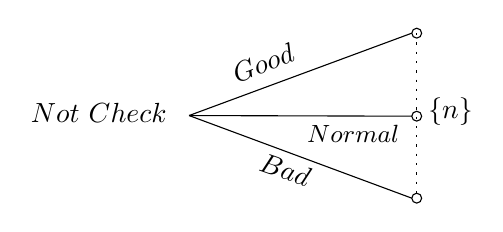
\begin{tikzpicture}[x=0.75pt,y=0.75pt,yscale=-1,xscale=1]
				%uncomment if require: \path (0,300); %set diagram left start at 0, and has height of 300

				%Straight Lines [id:da9949056217510941] 
				\draw    (267.33,117.1) -- (374.63,77.41) ;
				%Straight Lines [id:da0432033074054432] 
				\draw    (267.33,117.1) -- (374.63,156.91) ;
				%Straight Lines [id:da32517464762283166] 
				\draw    (267.33,117.1) -- (374.63,117.41) ;
				%Straight Lines [id:da5711505161730053] 
				\draw  [dash pattern={on 0.84pt off 2.51pt}]  (377,77.41) -- (377,156.91) ;
				%Shape: Circle [id:dp5888816527019345] 
				\draw   (374.63,77.41) .. controls (374.63,76.09) and (375.69,75.03) .. (377,75.03) .. controls (378.31,75.03) and (379.38,76.09) .. (379.38,77.41) .. controls (379.38,78.72) and (378.31,79.78) .. (377,79.78) .. controls (375.69,79.78) and (374.63,78.72) .. (374.63,77.41) -- cycle ;
				%Shape: Circle [id:dp6462591446600507] 
				\draw   (374.63,117.41) .. controls (374.63,116.09) and (375.69,115.03) .. (377,115.03) .. controls (378.31,115.03) and (379.38,116.09) .. (379.38,117.41) .. controls (379.38,118.72) and (378.31,119.78) .. (377,119.78) .. controls (375.69,119.78) and (374.63,118.72) .. (374.63,117.41) -- cycle ;
				%Shape: Circle [id:dp20344233868873163] 
				\draw   (374.63,156.91) .. controls (374.63,155.59) and (375.69,154.53) .. (377,154.53) .. controls (378.31,154.53) and (379.38,155.59) .. (379.38,156.91) .. controls (379.38,158.22) and (378.31,159.28) .. (377,159.28) .. controls (375.69,159.28) and (374.63,158.22) .. (374.63,156.91) -- cycle ;

				% Text Node
				\draw (285.54,92.19) node [anchor=north west][inner sep=0.75pt]  [rotate=-339.07]  {$Good$};
				% Text Node
				\draw (322.98,120.65) node [anchor=north west][inner sep=0.75pt]  [font=\small]  {$Normal$};
				% Text Node
				\draw (189.83,109.7) node [anchor=north west][inner sep=0.75pt]    {$Not\ Check$};
				% Text Node
				\draw (302.77,133.06) node [anchor=north west][inner sep=0.75pt]  [rotate=-19.16]  {$Bad$};
				% Text Node
				\draw (381.33,107.4) node [anchor=north west][inner sep=0.75pt]    {$\{n \}$};


			\end{tikzpicture}
		\end{minipage}
	\end{table}

	\vfill

	Preferences over financial gains and beliefs are:

	\vfill

	\[
		u \left( x; \ell \right) = v \left( x \right) + p_{\ell} \left( \text{Good} \right).
	\] \pause

	\vfill

	The investor expects to distort \( \ell \) so that \( p_{\ell^{*}} \left( Good \right) = 1 \).

	\vfill

	Optimistic beliefs lead her to invest more than what prescribed by Bayes rule.
\end{frame}

\begin{frame}{BDP imply non-Bayesian updating}

	Say the true likelihood \( \textcolor{RoyalBlue}{\ell} \) coincides with the distorted \( \textcolor{red}{\ell^{*}} \):

	\vfill

	\[
		\begin{aligned}
			\mathcal{U} \left(M ; \textcolor{RoyalBlue}{\ell} \right) = \max _{f \in M}\left\{\sum_{s} p_{\textcolor{RoyalBlue}{\ell}} \left( s \right) u \left( f_{s} ; \textcolor{RoyalBlue}{\ell} \right) + \right. & \left. \alpha_{\ell} \sum_{s} p_{\textcolor{RoyalBlue}{\ell}} \left( s \right) u \left( f_{s} ; \textcolor{RoyalBlue}{\ell} \right) \right\} \\
			-\max _{f^{\prime} \in M}                                                                                                                                                                                  & \: \alpha _{\ell} \sum_{s} p_{\textcolor{RoyalBlue}{\ell}} \left( s \right) u\left(f^{\prime}_{s} ; \textcolor{RoyalBlue}{\ell} \right) .
		\end{aligned}
	\]

	\vfill

	The second and third terms cancel out, only EU under Bayesian updating remains. \pause

	\vfill

	If \( u \) does not depend on \( \ell \), preferences over likelihoods are flat.

	\vfill
	A novelty of the model is that BDP \textbf{imply} non-Bayesian updating.

\end{frame}

\section{Main axioms and result}

\begin{frame}{Axiom: Identical Inference Independence}\label{independence}

	\begin{axiom}\label{ax:independence} (\textbf{Informal})
		The individual only satisfies independence for mixtures of contingent menus inducing the same inference for each of their menu realisations. \: \: \hyperlink{independenceapp}{\beamerbutton{Full}}
	\end{axiom}

	\vfill

	\begin{table}[H]
		\centering
		\begin{minipage}{0.29\textwidth}

		\end{minipage}\hspace{0.3cm} % Adjust the horizontal space between the tables and the symbol
		% Symbol goes here
		\begin{minipage}{0.29\textwidth}
			\centering
			\begin{tikzpicture}[x=0.75pt,y=0.75pt,yscale=-1,xscale=1]
				%uncomment if require: \path (0,341); %set diagram left start at 0, and has height of 341

				%Straight Lines [id:da6521689763503256] 
				\draw [color=Black, draw opacity=1]   (259.33,139.1) -- (366.63,99.41) ;
				%Straight Lines [id:da3094065715046459] 
				\draw [color=Black, draw opacity=1]   (259.33,139.1) -- (366.63,178.91) ;
				%Straight Lines [id:da3636097363244992] 
				\draw [color=Black, draw opacity=1]   (259.33,139.1) -- (366.63,139.41) ;
				%Straight Lines [id:da7301255340273027] 
				\draw  [dash pattern={on 0.84pt off 2.51pt}]  (369,99.41) -- (369,139.41) ;
				%Shape: Circle [id:dp5572573680385027] 
				\draw   (366.63,99.41) .. controls (366.63,98.09) and (367.69,97.03) .. (369,97.03) .. controls (370.31,97.03) and (371.38,98.09) .. (371.38,99.41) .. controls (371.38,100.72) and (370.31,101.78) .. (369,101.78) .. controls (367.69,101.78) and (366.63,100.72) .. (366.63,99.41) -- cycle ;
				%Shape: Circle [id:dp045414237311399264] 
				\draw   (366.63,139.41) .. controls (366.63,138.09) and (367.69,137.03) .. (369,137.03) .. controls (370.31,137.03) and (371.38,138.09) .. (371.38,139.41) .. controls (371.38,140.72) and (370.31,141.78) .. (369,141.78) .. controls (367.69,141.78) and (366.63,140.72) .. (366.63,139.41) -- cycle ;
				%Shape: Circle [id:dp6206756734194616] 
				\draw   (366.63,178.91) .. controls (366.63,177.59) and (367.69,176.53) .. (369,176.53) .. controls (370.31,176.53) and (371.38,177.59) .. (371.38,178.91) .. controls (371.38,180.22) and (370.31,181.28) .. (369,181.28) .. controls (367.69,181.28) and (366.63,180.22) .. (366.63,178.91) -- cycle ;

				% Text Node
				\draw (277.54,114.19) node [anchor=north west][inner sep=0.75pt]  [color=Black ,opacity=1 ,rotate=-339.07]  {$Good$};
				% Text Node
				\draw (314.98,142.65) node [anchor=north west][inner sep=0.75pt]  [font=\small,color=Black ,opacity=1 ]  {$Normal$};
				% Text Node
				\draw (211.83,130.7) node [anchor=north west][inner sep=0.75pt]    {};
				% Text Node
				\draw (294.77,155.06) node [anchor=north west][inner sep=0.75pt]  [color=Black ,opacity=1 ,rotate=-19.16]  {$Bad$};
				% Text Node
				\draw (371.33,156.4) node [anchor=north west][inner sep=0.75pt]  [color=Black ,opacity=1 ]  {$\overset{\underline{p}}{\{i, n\}}$};
				% Text Node
				\draw (370.83,98.4) node [anchor=north west][inner sep=0.75pt]  [color=Black ,opacity=1 ]  {$\overset{\overline{p}}{\{n\}}$};

			\end{tikzpicture}
		\end{minipage}\hspace{2cm} % Adjust the horizontal space between the tables and the symbol
		\begin{minipage}{0.45\textwidth}
			\centering
			\begin{tikzpicture}[x=0.75pt,y=0.75pt,yscale=-1,xscale=1]
				%uncomment if require: \path (0,341); %set diagram left start at 0, and has height of 341

				%Straight Lines [id:da6521689763503256] 
				\draw [color=Black, draw opacity=1]   (259.33,139.1) -- (366.63,99.41) ;
				%Straight Lines [id:da3094065715046459] 
				\draw [color=Black, draw opacity=1]   (259.33,139.1) -- (366.63,178.91) ;
				%Straight Lines [id:da3636097363244992] 
				\draw [color=Black, draw opacity=1]   (259.33,139.1) -- (366.63,139.41) ;
				%Straight Lines [id:da7301255340273027] 
				\draw  [dash pattern={on 0.84pt off 2.51pt}]  (369,99.41) -- (369,139.41) ;
				%Shape: Circle [id:dp5572573680385027] 
				\draw   (366.63,99.41) .. controls (366.63,98.09) and (367.69,97.03) .. (369,97.03) .. controls (370.31,97.03) and (371.38,98.09) .. (371.38,99.41) .. controls (371.38,100.72) and (370.31,101.78) .. (369,101.78) .. controls (367.69,101.78) and (366.63,100.72) .. (366.63,99.41) -- cycle ;
				%Shape: Circle [id:dp045414237311399264] 
				\draw   (366.63,139.41) .. controls (366.63,138.09) and (367.69,137.03) .. (369,137.03) .. controls (370.31,137.03) and (371.38,138.09) .. (371.38,139.41) .. controls (371.38,140.72) and (370.31,141.78) .. (369,141.78) .. controls (367.69,141.78) and (366.63,140.72) .. (366.63,139.41) -- cycle ;
				%Shape: Circle [id:dp6206756734194616] 
				\draw   (366.63,178.91) .. controls (366.63,177.59) and (367.69,176.53) .. (369,176.53) .. controls (370.31,176.53) and (371.38,177.59) .. (371.38,178.91) .. controls (371.38,180.22) and (370.31,181.28) .. (369,181.28) .. controls (367.69,181.28) and (366.63,180.22) .. (366.63,178.91) -- cycle ;

				% Text Node
				\draw (277.54,114.19) node [anchor=north west][inner sep=0.75pt]  [color=Black ,opacity=1 ,rotate=-339.07]  {$Good$};
				% Text Node
				\draw (314.98,142.65) node [anchor=north west][inner sep=0.75pt]  [font=\small,color=Black ,opacity=1 ]  {$Normal$};
				% Text Node
				\draw (211.83,130.7) node [anchor=north west][inner sep=0.75pt]    {};
				% Text Node
				\draw (294.77,155.06) node [anchor=north west][inner sep=0.75pt]  [color=Black ,opacity=1 ,rotate=-19.16]  {$Bad$};
				% Text Node
				\draw (371.33,156.4) node [anchor=north west][inner sep=0.75pt]  [color=Black ,opacity=1 ]  {$\overset{\underline{p}}{\{i ,n\}}$};
				% Text Node
				\draw (370.83,98.4) node [anchor=north west][inner sep=0.75pt]  [color=Black ,opacity=1 ]  {$\overset{\overline{p}}{\{\textcolor{RoyalBlue}{i} ,n\}}$};

			\end{tikzpicture}
		\end{minipage}
	\end{table} \pause

	\vfill

	Relaxing independence leads to dynamic inconsistency.

\end{frame}

\begin{frame}{Main Axiom: Strategic Rationality for Best Likelihood}\label{srbl}

	\begin{axiom}\label{ax:srbl} (\textbf{Informal})
		There is no temptation when, all else equal, the available menu comprises the best choices based on both the Bayesian update and the favourite posterior. \: \: \hyperlink{srblapp}{\beamerbutton{Full}} \pause
	\end{axiom}

	\vfill

	\begin{table}[H]
		\centering
		\begin{minipage}{0.29\textwidth}

		\end{minipage}\hspace{0.3cm} % Adjust the horizontal space between the tables and the symbol
		% Symbol goes here
		\begin{minipage}{0.29\textwidth}
			\centering
			\begin{tikzpicture}[x=0.75pt,y=0.75pt,yscale=-1,xscale=1]
				%uncomment if require: \path (0,341); %set diagram left start at 0, and has height of 341

				%Straight Lines [id:da6521689763503256] 
				\draw [color=Black, draw opacity=1]   (259.33,139.1) -- (366.63,99.41) ;
				%Straight Lines [id:da3094065715046459] 
				\draw [color=Black, draw opacity=1]   (259.33,139.1) -- (366.63,178.91) ;
				%Straight Lines [id:da3636097363244992] 
				\draw [color=Black, draw opacity=1]   (259.33,139.1) -- (366.63,139.41) ;
				%Straight Lines [id:da7301255340273027] 
				\draw  [dash pattern={on 0.84pt off 2.51pt}]  (369,99.41) -- (369,139.41) ;
				%Shape: Circle [id:dp5572573680385027] 
				\draw   (366.63,99.41) .. controls (366.63,98.09) and (367.69,97.03) .. (369,97.03) .. controls (370.31,97.03) and (371.38,98.09) .. (371.38,99.41) .. controls (371.38,100.72) and (370.31,101.78) .. (369,101.78) .. controls (367.69,101.78) and (366.63,100.72) .. (366.63,99.41) -- cycle ;
				%Shape: Circle [id:dp045414237311399264] 
				\draw   (366.63,139.41) .. controls (366.63,138.09) and (367.69,137.03) .. (369,137.03) .. controls (370.31,137.03) and (371.38,138.09) .. (371.38,139.41) .. controls (371.38,140.72) and (370.31,141.78) .. (369,141.78) .. controls (367.69,141.78) and (366.63,140.72) .. (366.63,139.41) -- cycle ;
				%Shape: Circle [id:dp6206756734194616] 
				\draw   (366.63,178.91) .. controls (366.63,177.59) and (367.69,176.53) .. (369,176.53) .. controls (370.31,176.53) and (371.38,177.59) .. (371.38,178.91) .. controls (371.38,180.22) and (370.31,181.28) .. (369,181.28) .. controls (367.69,181.28) and (366.63,180.22) .. (366.63,178.91) -- cycle ;

				% Text Node
				\draw (277.54,114.19) node [anchor=north west][inner sep=0.75pt]  [color=Black ,opacity=1 ,rotate=-339.07]  {$Good$};
				% Text Node
				\draw (314.98,142.65) node [anchor=north west][inner sep=0.75pt]  [font=\small,color=Black ,opacity=1 ]  {$Normal$};
				% Text Node
				\draw (211.83,130.7) node [anchor=north west][inner sep=0.75pt]    {};
				% Text Node
				\draw (294.77,155.06) node [anchor=north west][inner sep=0.75pt]  [color=Black ,opacity=1 ,rotate=-19.16]  {$Bad$};
				% Text Node
				\draw (371.33,156.4) node [anchor=north west][inner sep=0.75pt]  [color=Black ,opacity=1 ]  {$\overset{\underline{p}}{\{i, n\}}$};
				% Text Node
				\draw (370.83,98.4) node [anchor=north west][inner sep=0.75pt]  [color=Black ,opacity=1 ]  {$\overset{\overline{p}}{\{n\}}$};

			\end{tikzpicture}
		\end{minipage}\hspace{2cm} % Adjust the horizontal space between the tables and the symbol
		\begin{minipage}{0.45\textwidth}
			\centering
			\begin{tikzpicture}[x=0.75pt,y=0.75pt,yscale=-1,xscale=1]
				%uncomment if require: \path (0,341); %set diagram left start at 0, and has height of 341

				%Straight Lines [id:da6521689763503256] 
				\draw [color=Black, draw opacity=1]   (259.33,139.1) -- (366.63,99.41) ;
				%Straight Lines [id:da3094065715046459] 
				\draw [color=Black, draw opacity=1]   (259.33,139.1) -- (366.63,178.91) ;
				%Straight Lines [id:da3636097363244992] 
				\draw [color=Black, draw opacity=1]   (259.33,139.1) -- (366.63,139.41) ;
				%Straight Lines [id:da7301255340273027] 
				\draw  [dash pattern={on 0.84pt off 2.51pt}]  (369,99.41) -- (369,139.41) ;
				%Shape: Circle [id:dp5572573680385027] 
				\draw   (366.63,99.41) .. controls (366.63,98.09) and (367.69,97.03) .. (369,97.03) .. controls (370.31,97.03) and (371.38,98.09) .. (371.38,99.41) .. controls (371.38,100.72) and (370.31,101.78) .. (369,101.78) .. controls (367.69,101.78) and (366.63,100.72) .. (366.63,99.41) -- cycle ;
				%Shape: Circle [id:dp045414237311399264] 
				\draw   (366.63,139.41) .. controls (366.63,138.09) and (367.69,137.03) .. (369,137.03) .. controls (370.31,137.03) and (371.38,138.09) .. (371.38,139.41) .. controls (371.38,140.72) and (370.31,141.78) .. (369,141.78) .. controls (367.69,141.78) and (366.63,140.72) .. (366.63,139.41) -- cycle ;
				%Shape: Circle [id:dp6206756734194616] 
				\draw   (366.63,178.91) .. controls (366.63,177.59) and (367.69,176.53) .. (369,176.53) .. controls (370.31,176.53) and (371.38,177.59) .. (371.38,178.91) .. controls (371.38,180.22) and (370.31,181.28) .. (369,181.28) .. controls (367.69,181.28) and (366.63,180.22) .. (366.63,178.91) -- cycle ;

				% Text Node
				\draw (277.54,114.19) node [anchor=north west][inner sep=0.75pt]  [color=Black ,opacity=1 ,rotate=-339.07]  {$Good$};
				% Text Node
				\draw (314.98,142.65) node [anchor=north west][inner sep=0.75pt]  [font=\small,color=Black ,opacity=1 ]  {$Normal$};
				% Text Node
				\draw (211.83,130.7) node [anchor=north west][inner sep=0.75pt]    {};
				% Text Node
				\draw (294.77,155.06) node [anchor=north west][inner sep=0.75pt]  [color=Black ,opacity=1 ,rotate=-19.16]  {$Bad$};
				% Text Node
				\draw (371.33,156.4) node [anchor=north west][inner sep=0.75pt]  [color=Black ,opacity=1 ]  {$\overset{\underline{p}}{\{i ,n\}}$};
				% Text Node
				\draw (370.83,98.4) node [anchor=north west][inner sep=0.75pt]  [color=Black ,opacity=1 ]  {$\overset{\overline{p}}{\{\textcolor{RoyalBlue}{i} ,n\}}$};

			\end{tikzpicture}
		\end{minipage}
	\end{table}

\end{frame}

\begin{frame}[noframenumbering]{Main Axiom: Strategic Rationality for Best Likelihood}

	\begin{axiom}
		(\textbf{Informal}) There is no temptation when, all else equal, the available menu comprises the best choices based on both the Bayesian update and the favourite posterior. \: \: \hyperlink{srblapp}{\beamerbutton{Full}}
	\end{axiom}

	\vfill

	\begin{table}[H]
		\centering
		\begin{minipage}{0.29\textwidth}

		\end{minipage}\hspace{0.3cm} % Adjust the horizontal space between the tables and the symbol
		% Symbol goes here
		\begin{minipage}{0.29\textwidth}
			\centering
			\begin{tikzpicture}[x=0.75pt,y=0.75pt,yscale=-1,xscale=1]
				%uncomment if require: \path (0,341); %set diagram left start at 0, and has height of 341

				%Straight Lines [id:da6521689763503256] 
				\draw [color=Black, draw opacity=1]   (259.33,139.1) -- (366.63,99.41) ;
				%Straight Lines [id:da3094065715046459] 
				\draw [color=Black, draw opacity=1]   (259.33,139.1) -- (366.63,178.91) ;
				%Straight Lines [id:da3636097363244992] 
				\draw [color=Black, draw opacity=1]   (259.33,139.1) -- (366.63,139.41) ;
				%Straight Lines [id:da7301255340273027] 
				\draw  [dash pattern={on 0.84pt off 2.51pt}]  (369,99.41) -- (369,139.41) ;
				%Shape: Circle [id:dp5572573680385027] 
				\draw   (366.63,99.41) .. controls (366.63,98.09) and (367.69,97.03) .. (369,97.03) .. controls (370.31,97.03) and (371.38,98.09) .. (371.38,99.41) .. controls (371.38,100.72) and (370.31,101.78) .. (369,101.78) .. controls (367.69,101.78) and (366.63,100.72) .. (366.63,99.41) -- cycle ;
				%Shape: Circle [id:dp045414237311399264] 
				\draw   (366.63,139.41) .. controls (366.63,138.09) and (367.69,137.03) .. (369,137.03) .. controls (370.31,137.03) and (371.38,138.09) .. (371.38,139.41) .. controls (371.38,140.72) and (370.31,141.78) .. (369,141.78) .. controls (367.69,141.78) and (366.63,140.72) .. (366.63,139.41) -- cycle ;
				%Shape: Circle [id:dp6206756734194616] 
				\draw   (366.63,178.91) .. controls (366.63,177.59) and (367.69,176.53) .. (369,176.53) .. controls (370.31,176.53) and (371.38,177.59) .. (371.38,178.91) .. controls (371.38,180.22) and (370.31,181.28) .. (369,181.28) .. controls (367.69,181.28) and (366.63,180.22) .. (366.63,178.91) -- cycle ;

				% Text Node
				\draw (277.54,114.19) node [anchor=north west][inner sep=0.75pt]  [color=Black ,opacity=1 ,rotate=-339.07]  {$Good$};
				% Text Node
				\draw (314.98,142.65) node [anchor=north west][inner sep=0.75pt]  [font=\small,color=Black ,opacity=1 ]  {$Normal$};
				% Text Node
				\draw (211.83,130.7) node [anchor=north west][inner sep=0.75pt]    {};
				% Text Node
				\draw (294.77,155.06) node [anchor=north west][inner sep=0.75pt]  [color=Black ,opacity=1 ,rotate=-19.16]  {$Bad$};
				% Text Node
				\draw (371.33,156.4) node [anchor=north west][inner sep=0.75pt]  [color=Black ,opacity=1 ]  {$\overset{\underline{p}}{\{i, n\}}$};
				% Text Node
				\draw (370.83,98.4) node [anchor=north west][inner sep=0.75pt]  [color=Black ,opacity=1 ]  {$\overset{\overline{p}}{\{n\}}$};

			\end{tikzpicture}
		\end{minipage}\hspace{2cm} % Adjust the horizontal space between the tables and the symbol
		\( \succ \)
		\begin{minipage}{0.45\textwidth}
			\centering
			\begin{tikzpicture}[x=0.75pt,y=0.75pt,yscale=-1,xscale=1]
				%uncomment if require: \path (0,341); %set diagram left start at 0, and has height of 341

				%Straight Lines [id:da6521689763503256] 
				\draw [color=Black, draw opacity=1]   (259.33,139.1) -- (366.63,99.41) ;
				%Straight Lines [id:da3094065715046459] 
				\draw [color=Black, draw opacity=1]   (259.33,139.1) -- (366.63,178.91) ;
				%Straight Lines [id:da3636097363244992] 
				\draw [color=Black, draw opacity=1]   (259.33,139.1) -- (366.63,139.41) ;
				%Straight Lines [id:da7301255340273027] 
				\draw  [dash pattern={on 0.84pt off 2.51pt}]  (369,99.41) -- (369,139.41) ;
				%Shape: Circle [id:dp5572573680385027] 
				\draw   (366.63,99.41) .. controls (366.63,98.09) and (367.69,97.03) .. (369,97.03) .. controls (370.31,97.03) and (371.38,98.09) .. (371.38,99.41) .. controls (371.38,100.72) and (370.31,101.78) .. (369,101.78) .. controls (367.69,101.78) and (366.63,100.72) .. (366.63,99.41) -- cycle ;
				%Shape: Circle [id:dp045414237311399264] 
				\draw   (366.63,139.41) .. controls (366.63,138.09) and (367.69,137.03) .. (369,137.03) .. controls (370.31,137.03) and (371.38,138.09) .. (371.38,139.41) .. controls (371.38,140.72) and (370.31,141.78) .. (369,141.78) .. controls (367.69,141.78) and (366.63,140.72) .. (366.63,139.41) -- cycle ;
				%Shape: Circle [id:dp6206756734194616] 
				\draw   (366.63,178.91) .. controls (366.63,177.59) and (367.69,176.53) .. (369,176.53) .. controls (370.31,176.53) and (371.38,177.59) .. (371.38,178.91) .. controls (371.38,180.22) and (370.31,181.28) .. (369,181.28) .. controls (367.69,181.28) and (366.63,180.22) .. (366.63,178.91) -- cycle ;

				% Text Node
				\draw (277.54,114.19) node [anchor=north west][inner sep=0.75pt]  [color=Black ,opacity=1 ,rotate=-339.07]  {$Good$};
				% Text Node
				\draw (314.98,142.65) node [anchor=north west][inner sep=0.75pt]  [font=\small,color=Black ,opacity=1 ]  {$Normal$};
				% Text Node
				\draw (211.83,130.7) node [anchor=north west][inner sep=0.75pt]    {};
				% Text Node
				\draw (294.77,155.06) node [anchor=north west][inner sep=0.75pt]  [color=Black ,opacity=1 ,rotate=-19.16]  {$Bad$};
				% Text Node
				\draw (371.33,156.4) node [anchor=north west][inner sep=0.75pt]  [color=Black ,opacity=1 ]  {$\overset{\underline{p}}{\{i ,n\}}$};
				% Text Node
				\draw (370.83,98.4) node [anchor=north west][inner sep=0.75pt]  [color=Black ,opacity=1 ]  {$\overset{\overline{p}}{\{\textcolor{RoyalBlue}{i} ,n\}}$};

			\end{tikzpicture}
		\end{minipage}
	\end{table}


\end{frame}

\begin{frame}[noframenumbering]{Main Axiom: Strategic Rationality for Best Likelihood}

	\begin{axiom}
		(\textbf{Informal}) There is no temptation when, all else equal, the available menu comprises the best choices based on both the Bayesian update and the favourite posterior. \: \: \hyperlink{srblapp}{\beamerbutton{Full}}
	\end{axiom}

	\vfill

	\begin{table}[H]
		\centering
		\begin{minipage}{0.29\textwidth}

		\end{minipage}\hspace{0.3cm} % Adjust the horizontal space between the tables and the symbol
		% Symbol goes here
		\begin{minipage}{0.29\textwidth}
			\centering
			\begin{tikzpicture}[x=0.75pt,y=0.75pt,yscale=-1,xscale=1]
				%uncomment if require: \path (0,341); %set diagram left start at 0, and has height of 341

				%Straight Lines [id:da6521689763503256] 
				\draw [color=Black, draw opacity=1]   (259.33,139.1) -- (366.63,99.41) ;
				%Straight Lines [id:da3094065715046459] 
				\draw [color=Black, draw opacity=1]   (259.33,139.1) -- (366.63,178.91) ;
				%Straight Lines [id:da3636097363244992] 
				\draw [color=Black, draw opacity=1]   (259.33,139.1) -- (366.63,139.41) ;
				%Straight Lines [id:da7301255340273027] 
				\draw  [dash pattern={on 0.84pt off 2.51pt}]  (369,99.41) -- (369,139.41) ;
				%Shape: Circle [id:dp5572573680385027] 
				\draw   (366.63,99.41) .. controls (366.63,98.09) and (367.69,97.03) .. (369,97.03) .. controls (370.31,97.03) and (371.38,98.09) .. (371.38,99.41) .. controls (371.38,100.72) and (370.31,101.78) .. (369,101.78) .. controls (367.69,101.78) and (366.63,100.72) .. (366.63,99.41) -- cycle ;
				%Shape: Circle [id:dp045414237311399264] 
				\draw   (366.63,139.41) .. controls (366.63,138.09) and (367.69,137.03) .. (369,137.03) .. controls (370.31,137.03) and (371.38,138.09) .. (371.38,139.41) .. controls (371.38,140.72) and (370.31,141.78) .. (369,141.78) .. controls (367.69,141.78) and (366.63,140.72) .. (366.63,139.41) -- cycle ;
				%Shape: Circle [id:dp6206756734194616] 
				\draw   (366.63,178.91) .. controls (366.63,177.59) and (367.69,176.53) .. (369,176.53) .. controls (370.31,176.53) and (371.38,177.59) .. (371.38,178.91) .. controls (371.38,180.22) and (370.31,181.28) .. (369,181.28) .. controls (367.69,181.28) and (366.63,180.22) .. (366.63,178.91) -- cycle ;

				% Text Node
				\draw (277.54,114.19) node [anchor=north west][inner sep=0.75pt]  [color=Black ,opacity=1 ,rotate=-339.07]  {$Good$};
				% Text Node
				\draw (314.98,142.65) node [anchor=north west][inner sep=0.75pt]  [font=\small,color=Black ,opacity=1 ]  {$Normal$};
				% Text Node
				\draw (211.83,130.7) node [anchor=north west][inner sep=0.75pt]    {};
				% Text Node
				\draw (294.77,155.06) node [anchor=north west][inner sep=0.75pt]  [color=Black ,opacity=1 ,rotate=-19.16]  {$Bad$};
				% Text Node
				\draw (371.33,156.4) node [anchor=north west][inner sep=0.75pt]  [color=Black ,opacity=1 ]  {$\overset{\underline{p}}{\{i, n\}}$};
				% Text Node
				\draw (370.83,98.4) node [anchor=north west][inner sep=0.75pt]  [color=Black ,opacity=1 ]  {$\overset{\overline{p}}{\{n\}}$};

			\end{tikzpicture}
		\end{minipage}\hspace{2cm} % Adjust the horizontal space between the tables and the symbol
		\begin{minipage}{0.45\textwidth}
			\centering
			\begin{tikzpicture}[x=0.75pt,y=0.75pt,yscale=-1,xscale=1]
				%uncomment if require: \path (0,341); %set diagram left start at 0, and has height of 341

				%Straight Lines [id:da6521689763503256] 
				\draw [color=Black, draw opacity=1]   (259.33,139.1) -- (366.63,99.41) ;
				%Straight Lines [id:da3094065715046459] 
				\draw [color=Black, draw opacity=1]   (259.33,139.1) -- (366.63,178.91) ;
				%Straight Lines [id:da3636097363244992] 
				\draw [color=Black, draw opacity=1]   (259.33,139.1) -- (366.63,139.41) ;
				%Straight Lines [id:da7301255340273027] 
				\draw  [dash pattern={on 0.84pt off 2.51pt}]  (369,99.41) -- (369,139.41) ;
				%Shape: Circle [id:dp5572573680385027] 
				\draw   (366.63,99.41) .. controls (366.63,98.09) and (367.69,97.03) .. (369,97.03) .. controls (370.31,97.03) and (371.38,98.09) .. (371.38,99.41) .. controls (371.38,100.72) and (370.31,101.78) .. (369,101.78) .. controls (367.69,101.78) and (366.63,100.72) .. (366.63,99.41) -- cycle ;
				%Shape: Circle [id:dp045414237311399264] 
				\draw   (366.63,139.41) .. controls (366.63,138.09) and (367.69,137.03) .. (369,137.03) .. controls (370.31,137.03) and (371.38,138.09) .. (371.38,139.41) .. controls (371.38,140.72) and (370.31,141.78) .. (369,141.78) .. controls (367.69,141.78) and (366.63,140.72) .. (366.63,139.41) -- cycle ;
				%Shape: Circle [id:dp6206756734194616] 
				\draw   (366.63,178.91) .. controls (366.63,177.59) and (367.69,176.53) .. (369,176.53) .. controls (370.31,176.53) and (371.38,177.59) .. (371.38,178.91) .. controls (371.38,180.22) and (370.31,181.28) .. (369,181.28) .. controls (367.69,181.28) and (366.63,180.22) .. (366.63,178.91) -- cycle ;

				% Text Node
				\draw (277.54,114.19) node [anchor=north west][inner sep=0.75pt]  [color=Black ,opacity=1 ,rotate=-339.07]  {$Good$};
				% Text Node
				\draw (314.98,142.65) node [anchor=north west][inner sep=0.75pt]  [font=\small,color=Black ,opacity=1 ]  {$Normal$};
				% Text Node
				\draw (211.83,130.7) node [anchor=north west][inner sep=0.75pt]    {};
				% Text Node
				\draw (294.77,155.06) node [anchor=north west][inner sep=0.75pt]  [color=Black ,opacity=1 ,rotate=-19.16]  {$Bad$};
				% Text Node
				\draw (371.33,156.4) node [anchor=north west][inner sep=0.75pt]  [color=Black ,opacity=1 ]  {$\overset{\underline{p}}{\{i ,n\}}$};
				% Text Node
				\draw (370.83,98.4) node [anchor=north west][inner sep=0.75pt]  [color=Black ,opacity=1 ]  {$\overset{\overline{p}}{\{\textcolor{RoyalBlue}{w} ,n\}}$};

			\end{tikzpicture}
		\end{minipage}
	\end{table}
\end{frame}

\begin{frame}[noframenumbering]{Main Axiom: Strategic Rationality for Best Likelihood}

	\begin{axiom}
		(\textbf{Informal}) There is no temptation when, all else equal, the available menu comprises the best choices based on both the Bayesian update and the favourite posterior. \: \: \hyperlink{srblapp}{\beamerbutton{Full}}
	\end{axiom}

	\vfill

	\begin{table}[H]
		\centering
		\begin{minipage}{0.29\textwidth}

		\end{minipage}\hspace{0.3cm} % Adjust the horizontal space between the tables and the symbol
		% Symbol goes here
		\begin{minipage}{0.29\textwidth}
			\centering
			\begin{tikzpicture}[x=0.75pt,y=0.75pt,yscale=-1,xscale=1]
				%uncomment if require: \path (0,341); %set diagram left start at 0, and has height of 341

				%Straight Lines [id:da6521689763503256] 
				\draw [color=Black, draw opacity=1]   (259.33,139.1) -- (366.63,99.41) ;
				%Straight Lines [id:da3094065715046459] 
				\draw [color=Black, draw opacity=1]   (259.33,139.1) -- (366.63,178.91) ;
				%Straight Lines [id:da3636097363244992] 
				\draw [color=Black, draw opacity=1]   (259.33,139.1) -- (366.63,139.41) ;
				%Straight Lines [id:da7301255340273027] 
				\draw  [dash pattern={on 0.84pt off 2.51pt}]  (369,99.41) -- (369,139.41) ;
				%Shape: Circle [id:dp5572573680385027] 
				\draw   (366.63,99.41) .. controls (366.63,98.09) and (367.69,97.03) .. (369,97.03) .. controls (370.31,97.03) and (371.38,98.09) .. (371.38,99.41) .. controls (371.38,100.72) and (370.31,101.78) .. (369,101.78) .. controls (367.69,101.78) and (366.63,100.72) .. (366.63,99.41) -- cycle ;
				%Shape: Circle [id:dp045414237311399264] 
				\draw   (366.63,139.41) .. controls (366.63,138.09) and (367.69,137.03) .. (369,137.03) .. controls (370.31,137.03) and (371.38,138.09) .. (371.38,139.41) .. controls (371.38,140.72) and (370.31,141.78) .. (369,141.78) .. controls (367.69,141.78) and (366.63,140.72) .. (366.63,139.41) -- cycle ;
				%Shape: Circle [id:dp6206756734194616] 
				\draw   (366.63,178.91) .. controls (366.63,177.59) and (367.69,176.53) .. (369,176.53) .. controls (370.31,176.53) and (371.38,177.59) .. (371.38,178.91) .. controls (371.38,180.22) and (370.31,181.28) .. (369,181.28) .. controls (367.69,181.28) and (366.63,180.22) .. (366.63,178.91) -- cycle ;

				% Text Node
				\draw (277.54,114.19) node [anchor=north west][inner sep=0.75pt]  [color=Black ,opacity=1 ,rotate=-339.07]  {$Good$};
				% Text Node
				\draw (314.98,142.65) node [anchor=north west][inner sep=0.75pt]  [font=\small,color=Black ,opacity=1 ]  {$Normal$};
				% Text Node
				\draw (211.83,130.7) node [anchor=north west][inner sep=0.75pt]    {};
				% Text Node
				\draw (294.77,155.06) node [anchor=north west][inner sep=0.75pt]  [color=Black ,opacity=1 ,rotate=-19.16]  {$Bad$};
				% Text Node
				\draw (371.33,156.4) node [anchor=north west][inner sep=0.75pt]  [color=Black ,opacity=1 ]  {$\overset{\underline{p}}{\{i, n\}}$};
				% Text Node
				\draw (370.83,98.4) node [anchor=north west][inner sep=0.75pt]  [color=Black ,opacity=1 ]  {$\overset{\overline{p}}{\{n\}}$};

			\end{tikzpicture}
		\end{minipage}\hspace{2cm} % Adjust the horizontal space between the tables and the symbol
		\( \sim \)
		\begin{minipage}{0.45\textwidth}
			\centering
			\begin{tikzpicture}[x=0.75pt,y=0.75pt,yscale=-1,xscale=1]
				%uncomment if require: \path (0,341); %set diagram left start at 0, and has height of 341

				%Straight Lines [id:da6521689763503256] 
				\draw [color=Black, draw opacity=1]   (259.33,139.1) -- (366.63,99.41) ;
				%Straight Lines [id:da3094065715046459] 
				\draw [color=Black, draw opacity=1]   (259.33,139.1) -- (366.63,178.91) ;
				%Straight Lines [id:da3636097363244992] 
				\draw [color=Black, draw opacity=1]   (259.33,139.1) -- (366.63,139.41) ;
				%Straight Lines [id:da7301255340273027] 
				\draw  [dash pattern={on 0.84pt off 2.51pt}]  (369,99.41) -- (369,139.41) ;
				%Shape: Circle [id:dp5572573680385027] 
				\draw   (366.63,99.41) .. controls (366.63,98.09) and (367.69,97.03) .. (369,97.03) .. controls (370.31,97.03) and (371.38,98.09) .. (371.38,99.41) .. controls (371.38,100.72) and (370.31,101.78) .. (369,101.78) .. controls (367.69,101.78) and (366.63,100.72) .. (366.63,99.41) -- cycle ;
				%Shape: Circle [id:dp045414237311399264] 
				\draw   (366.63,139.41) .. controls (366.63,138.09) and (367.69,137.03) .. (369,137.03) .. controls (370.31,137.03) and (371.38,138.09) .. (371.38,139.41) .. controls (371.38,140.72) and (370.31,141.78) .. (369,141.78) .. controls (367.69,141.78) and (366.63,140.72) .. (366.63,139.41) -- cycle ;
				%Shape: Circle [id:dp6206756734194616] 
				\draw   (366.63,178.91) .. controls (366.63,177.59) and (367.69,176.53) .. (369,176.53) .. controls (370.31,176.53) and (371.38,177.59) .. (371.38,178.91) .. controls (371.38,180.22) and (370.31,181.28) .. (369,181.28) .. controls (367.69,181.28) and (366.63,180.22) .. (366.63,178.91) -- cycle ;

				% Text Node
				\draw (277.54,114.19) node [anchor=north west][inner sep=0.75pt]  [color=Black ,opacity=1 ,rotate=-339.07]  {$Good$};
				% Text Node
				\draw (314.98,142.65) node [anchor=north west][inner sep=0.75pt]  [font=\small,color=Black ,opacity=1 ]  {$Normal$};
				% Text Node
				\draw (211.83,130.7) node [anchor=north west][inner sep=0.75pt]    {};
				% Text Node
				\draw (294.77,155.06) node [anchor=north west][inner sep=0.75pt]  [color=Black ,opacity=1 ,rotate=-19.16]  {$Bad$};
				% Text Node
				\draw (371.33,156.4) node [anchor=north west][inner sep=0.75pt]  [color=Black ,opacity=1 ]  {$\overset{\underline{p}}{\{i ,n\}}$};
				% Text Node
				\draw (370.83,98.4) node [anchor=north west][inner sep=0.75pt]  [color=Black ,opacity=1 ]  {$\overset{\overline{p}}{\{\textcolor{RoyalBlue}{w} ,n\}}$};

			\end{tikzpicture}
		\end{minipage}
	\end{table} \pause

	\vfill

	Under no BDP, all posteriors are "favourite" and the axiom implies no temptation.

	\vfill

	No temptation implies the model reduces to Expected utility and Bayesian updating.
\end{frame}

\begin{frame}{Main Result}\label{mainresult}

	\begin{theorem}
		Preferences over contingent menus are represented by Equations (\ref{eq:contmenu}) and (\ref{eq:menu}) if and only if they satisfy \textbf{Strategic Rationality for Best Likelihood} and other "standard" axioms.
	\end{theorem}

	\vfill

	\begin{equation}\label{eq:contmenu}
		\mathscr{U}(F)= \sum_{M} \sum_{s} p \left( s \right) F_{s} \left( M \right) \mathcal{U} \left(M ; \ell_{M, F} \right) .
	\end{equation}

	\vfill

	\begin{equation}\label{eq:menu}
		\begin{aligned}
			\mathcal{U} \left(M ; \ell \right) = \max _{f \in M}\left\{\sum_{s} p_{\ell} \left( s \right) u \left( f_{s} ; \ell \right) + \right. & \left. \alpha_{\ell} \sum_{s} p_{\ell^{*}_{S_{\ell}}} \left( s \right) u \left( f_{s} ; \ell^{*}_{S_{\ell}} \right) \right\} \\
			-\max _{f^{\prime} \in M}                                                                                                             & \: \alpha _{\ell} \sum_{s} p_{\ell^{*}_{S_{\ell}}} \left( s \right) u\left(f^{\prime}_{s} ; \ell^{*}_{S_{\ell}} \right) .
		\end{aligned}
	\end{equation}

	\vfill

	Prior belief \( p \), utilities \( u \), distorted likelihoods \( \ell^{*} \) and weights \( \alpha \) are unique. \hyperlink{axiomsb1main}{\beamerbutton{Axioms?}}

\end{frame}

\begin{frame}{Why this model}

	\begin{wideenumerate}
		\item Generality: how do individuals choose between information sources?
		\item Refutability: predictions of previous theories overlap, also with non BDP.
		\item Identification: how to intervene if preferences and beliefs are confused?
		\item Dual-self: which self matters for welfare analysis?
	\end{wideenumerate}

\end{frame}

\begin{comment}

\begin{frame}{Why this model: observability and identification}
	The primitive objects of choice, contingent menus, are observable, contrary to

	\vfill

	\begin{wideitemize}
		\item Choice of beliefs \citep{brunnermeierOptimalExpectations2005,koszegiUtilityAnticipationPersonal2010};
		\item Choice of probability to forget \citep{benabou2016mindful}.
	\end{wideitemize}

	\vfill

	Choices of information sources do not allow identification \citep{eliazCanAnticipatoryFeelings2006}.

	\vfill

	These papers only provide "if" results, hard to distinguish from other theories.
\end{frame}

\begin{frame}{Why this model: multiple selves and updating}
	Individual as the unit of choice:
	\vfill

	\begin{wideitemize}
		\item multiple selves render welfare analysis hard;
		\item under multiple selves, choices are dynamically inconsistent.
	\end{wideitemize}

	\vfill

	BDP and non-Bayesian updating are not disjoint, the first implies the second.
\end{frame}

\end{comment}


\begin{frame}{Conclusion}
	Theory of BDP and belief updating tested via choices of contingent menus:
	\vfill

	\begin{wideitemize}
		\item dynamically consistent individual anticipates she distorts beliefs;
		\item asymmetric updating and no distortion of zero probability events;
		\item identification of BDP, non-Bayesian updating and strength of motivated reasoning.
	\end{wideitemize}

	\vfill

	Other applications in the paper:

	\vfill

	\begin{wideitemize}
		\item donors avoid and distort information about their impact;
		\item politicians send poor information to induce polarisation.
	\end{wideitemize}

\end{frame}

\begin{frame}[noframenumbering,plain]

	\frametitle{References}

	%\nocite{*}
	\bibliography{Others/bib}
	\bibliographystyle{apacite}


\end{frame}

\appendix

\begin{frame}[noframenumbering,plain]{Cost of self-control}\label{alpha}

	Identification of \( \alpha_{\ell} \) allows elaborating on its behavioural meaning

	\vfill

	\[
		\alpha_{\ell} = \frac{\mathcal{U} \left( \left\{f; x \right\}, \ell \right) - \mathcal{U} \left( \left\{f; x^{\prime} \right\}, \ell \right) }{u \left( x ; \ell \right) - u \left( x^{\prime} ; \ell \right)} .
	\]

	\vfill

	It is the marginal cost of self-control at likelihood \( \ell \). \hyperlink{fullmodel}{\beamerbutton{Back}}

\end{frame}

\begin{frame}[noframenumbering,plain]{Alternative representation with cost}\label{cost}

	The representation can be written as either

	\[
		\begin{aligned}
			\mathcal{U} \left(M ; \ell \right) = \max _{f \in M}\left\{\sum_{s} p_{\ell} \left( s \right) u \left( f_{s} ; \ell \right) + \right. & \left. \alpha_{\ell} \sum_{s} p_{\ell^{*}_{S_{\ell}}} \left( s \right) u \left( f_{s} ; \ell^{*}_{S_{\ell}} \right) \right\} \\
			-\max _{f^{\prime} \in M}                                                                                                             & \: \alpha _{\ell} \sum_{s} p_{\ell^{*}_{S_{\ell}}} \left( s \right) u\left(f^{\prime}_{s} ; \ell^{*}_{S_{\ell}} \right)
		\end{aligned}
	\]

	or

	\[
		\mathcal{U} \left(M ; \ell \right) = \max _{f \in M}\left\{\sum_{s} p_{\ell} \left( s \right) u \left( f_{s} ; \ell \right) - \alpha_{\ell} \:  c \left( f, u, S_{\ell} \right) \right\} .
	\]

	\begin{flushright}
		\hyperlink{fullmodel}{\beamerbutton{Back}}
	\end{flushright}

\end{frame}

\begin{frame}[noframenumbering,plain]{Axioms: Basics (Informal)}\label{axiomsb1main}

	\begin{axiom}\label{ax:order}
		\labelname{axn:order}{Order and Continuity} (\textbf{Order}). Preferences over contingent menus are a continuous weak order. \hyperlink{axiomsb1}{\beamerbutton{Full}}
	\end{axiom}

	\begin{axiom}\label{ax:degeneracy}
		\labelname{axn:degeneracy}{Nondegeneracy}

		(\textbf{Nondegeneracy}). There exist at least one outcome better than another. \hyperlink{axiomsb2}{\beamerbutton{Full}}

	\end{axiom}

	\begin{axiom}\label{ax:sindependence}
		\labelname{axn:sindependence}{State Independence}

		(\textbf{\textbf{State Independence}}). Preferences over outcomes do not depend on the state.
	\end{axiom}

	\begin{axiom}\label{ax:support}
		\labelname{axn:support}{Full Support}

		(\textbf{\textbf{Full support}}). The individual assigns ex-ante positive probability to all states.
	\end{axiom}

	\begin{flushright}
		\hyperlink{mainresult}{\beamerbutton{Back}}
	\end{flushright}

\end{frame}

\begin{frame}[noframenumbering,plain]{Axioms: Set-Betweenness (Informal)}\label{betweenness}

	\begin{axiom}\label{ax:sbetweenness}
		The individual is weakly worse if a menu is enhanced with ex-ante dominated options, because these induce temptation.
	\end{axiom}

	\vfill

	\begin{table}[H]
		\centering
		\begin{minipage}{0.29\textwidth}

		\end{minipage}\hspace{0.3cm} % Adjust the horizontal space between the tables and the symbol
		% Symbol goes here
		\begin{minipage}{0.29\textwidth}
			\centering
			\begin{tikzpicture}[x=0.75pt,y=0.75pt,yscale=-1,xscale=1]
				%uncomment if require: \path (0,341); %set diagram left start at 0, and has height of 341

				%Straight Lines [id:da6521689763503256] 
				\draw [color=Black, draw opacity=1]   (259.33,139.1) -- (366.63,99.41) ;
				%Straight Lines [id:da3094065715046459] 
				\draw [color=Black, draw opacity=1]   (259.33,139.1) -- (366.63,178.91) ;
				%Straight Lines [id:da3636097363244992] 
				\draw [color=Black, draw opacity=1]   (259.33,139.1) -- (366.63,139.41) ;
				%Straight Lines [id:da7301255340273027] 
				\draw  [dash pattern={on 0.84pt off 2.51pt}]  (369,99.41) -- (369,139.41) ;
				%Shape: Circle [id:dp5572573680385027] 
				\draw   (366.63,99.41) .. controls (366.63,98.09) and (367.69,97.03) .. (369,97.03) .. controls (370.31,97.03) and (371.38,98.09) .. (371.38,99.41) .. controls (371.38,100.72) and (370.31,101.78) .. (369,101.78) .. controls (367.69,101.78) and (366.63,100.72) .. (366.63,99.41) -- cycle ;
				%Shape: Circle [id:dp045414237311399264] 
				\draw   (366.63,139.41) .. controls (366.63,138.09) and (367.69,137.03) .. (369,137.03) .. controls (370.31,137.03) and (371.38,138.09) .. (371.38,139.41) .. controls (371.38,140.72) and (370.31,141.78) .. (369,141.78) .. controls (367.69,141.78) and (366.63,140.72) .. (366.63,139.41) -- cycle ;
				%Shape: Circle [id:dp6206756734194616] 
				\draw   (366.63,178.91) .. controls (366.63,177.59) and (367.69,176.53) .. (369,176.53) .. controls (370.31,176.53) and (371.38,177.59) .. (371.38,178.91) .. controls (371.38,180.22) and (370.31,181.28) .. (369,181.28) .. controls (367.69,181.28) and (366.63,180.22) .. (366.63,178.91) -- cycle ;

				% Text Node
				\draw (277.54,114.19) node [anchor=north west][inner sep=0.75pt]  [color=Black ,opacity=1 ,rotate=-339.07]  {$Good$};
				% Text Node
				\draw (314.98,142.65) node [anchor=north west][inner sep=0.75pt]  [font=\small,color=Black ,opacity=1 ]  {$Normal$};
				% Text Node
				\draw (211.83,130.7) node [anchor=north west][inner sep=0.75pt]    {};
				% Text Node
				\draw (294.77,155.06) node [anchor=north west][inner sep=0.75pt]  [color=Black ,opacity=1 ,rotate=-19.16]  {$Bad$};
				% Text Node
				\draw (371.33,156.4) node [anchor=north west][inner sep=0.75pt]  [color=Black ,opacity=1 ]  {$\overset{\underline{p}}{\{i, n\}}$};
				% Text Node
				\draw (370.83,98.4) node [anchor=north west][inner sep=0.75pt]  [color=Black ,opacity=1 ]  {$\overset{\overline{p}}{\{n\}}$};

			\end{tikzpicture}
		\end{minipage}\hspace{2cm} % Adjust the horizontal space between the tables and the symbol
		\( \succ \)
		\begin{minipage}{0.45\textwidth}
			\centering
			\begin{tikzpicture}[x=0.75pt,y=0.75pt,yscale=-1,xscale=1]
				%uncomment if require: \path (0,341); %set diagram left start at 0, and has height of 341

				%Straight Lines [id:da6521689763503256] 
				\draw [color=Black, draw opacity=1]   (259.33,139.1) -- (366.63,99.41) ;
				%Straight Lines [id:da3094065715046459] 
				\draw [color=Black, draw opacity=1]   (259.33,139.1) -- (366.63,178.91) ;
				%Straight Lines [id:da3636097363244992] 
				\draw [color=Black, draw opacity=1]   (259.33,139.1) -- (366.63,139.41) ;
				%Straight Lines [id:da7301255340273027] 
				\draw  [dash pattern={on 0.84pt off 2.51pt}]  (369,99.41) -- (369,139.41) ;
				%Shape: Circle [id:dp5572573680385027] 
				\draw   (366.63,99.41) .. controls (366.63,98.09) and (367.69,97.03) .. (369,97.03) .. controls (370.31,97.03) and (371.38,98.09) .. (371.38,99.41) .. controls (371.38,100.72) and (370.31,101.78) .. (369,101.78) .. controls (367.69,101.78) and (366.63,100.72) .. (366.63,99.41) -- cycle ;
				%Shape: Circle [id:dp045414237311399264] 
				\draw   (366.63,139.41) .. controls (366.63,138.09) and (367.69,137.03) .. (369,137.03) .. controls (370.31,137.03) and (371.38,138.09) .. (371.38,139.41) .. controls (371.38,140.72) and (370.31,141.78) .. (369,141.78) .. controls (367.69,141.78) and (366.63,140.72) .. (366.63,139.41) -- cycle ;
				%Shape: Circle [id:dp6206756734194616] 
				\draw   (366.63,178.91) .. controls (366.63,177.59) and (367.69,176.53) .. (369,176.53) .. controls (370.31,176.53) and (371.38,177.59) .. (371.38,178.91) .. controls (371.38,180.22) and (370.31,181.28) .. (369,181.28) .. controls (367.69,181.28) and (366.63,180.22) .. (366.63,178.91) -- cycle ;

				% Text Node
				\draw (277.54,114.19) node [anchor=north west][inner sep=0.75pt]  [color=Black ,opacity=1 ,rotate=-339.07]  {$Good$};
				% Text Node
				\draw (314.98,142.65) node [anchor=north west][inner sep=0.75pt]  [font=\small,color=Black ,opacity=1 ]  {$Normal$};
				% Text Node
				\draw (211.83,130.7) node [anchor=north west][inner sep=0.75pt]    {};
				% Text Node
				\draw (294.77,155.06) node [anchor=north west][inner sep=0.75pt]  [color=Black ,opacity=1 ,rotate=-19.16]  {$Bad$};
				% Text Node
				\draw (371.33,156.4) node [anchor=north west][inner sep=0.75pt]  [color=Black ,opacity=1 ]  {$\overset{\underline{p}}{\{i ,n\}}$};
				% Text Node
				\draw (370.83,98.4) node [anchor=north west][inner sep=0.75pt]  [color=Black ,opacity=1 ]  {$\overset{\overline{p}}{\{\textcolor{RoyalBlue}{i} ,n\}}$};

			\end{tikzpicture}
		\end{minipage}
	\end{table}
	\begin{flushright}
		\hyperlink{betweennessapp}{\beamerbutton{Full}}
	\end{flushright}


\end{frame}

\begin{frame}[noframenumbering,plain]{Axioms: Basics I}

	\begin{axiom}\label{ax:orderapp}
		\labelname{axn:orderapp}{Order} (\textbf{Order}). The ranking \(\succsim\) is complete and transitive.

	\end{axiom}

	\vfill

	\begin{axiom}\label{ax:continuityapp}\label{axiomsb1}
		\labelname{axn:continuityapp}{Continuity}

		(\textbf{Continuity}). For all contingent menus \( F \) the sets

		\[
			\left\{ F^{\prime} \mid F^{\prime} \succsim F \right\} \: and \: \left\{ F^{\prime} \mid F^{\prime} \precsim F \right\}
		\]

		are closed.

	\end{axiom}

	\begin{flushright}
		\hyperlink{axiomsb1main}{\beamerbutton{Back}}
	\end{flushright}

\end{frame}

\begin{frame}[noframenumbering,plain]{Axioms: Basics II}\label{axiomsb2}

	Substitute from \( F \) any occurrence of \( M \) with \( M^{\prime} \) to get \( F_{M \rightarrow M^{\prime}} \).

	\vfill

	\begin{axiom}\label{ax:degeneracyapp}
		\labelname{axn:degeneracyapp}{Nondegeneracy}

		(\textbf{Nondegeneracy}). There exist outcomes \(y, y^{\prime}\) such that \(y \succ y^{\prime}\).

	\end{axiom}

	\vfill

	\begin{axiom}\label{ax:sindependenceapp}
		\labelname{axn:sindependenceapp}{State Independence}

		(\textbf{\textbf{State Independence}}). For all contingent menus \( F \), menus \( L, L^{\prime}, M \) and states \( s, s^{\prime} \),

		\[
			F \succsim F_{L s M \rightarrow L^{\prime} s M} \: \Rightarrow \: F \succsim F_{L s^{\prime} M \rightarrow L^{\prime} s^{\prime} M} .
		\]

	\end{axiom}


	\vfill

	\begin{axiom}\label{ax:appsupport}
		\labelname{axn:appsupport}{Full Support}

		(\textbf{\textbf{Full Support}}). For each state \(s\), there exist contingent menus \(F \) and \(F^{\prime}\) such that for all menus \( M \) it holds that \(F_{s^{\prime}} \left( M \right) =F^{\prime}_{s^{\prime}} \left( M \right)\) for every \(s^{\prime} \neq s \) and \(F \nsim F^{\prime}\).

	\end{axiom}

	\begin{flushright}
		\hyperlink{axiomsb1main}{\beamerbutton{Back}}
	\end{flushright}
\end{frame}

\begin{frame}[noframenumbering,plain]{Axioms: Identical Inference Independence}

	The support of \( F \) is

	\[ \mathcal{M}_{F} := \left\{ M \in \mathcal{M} \: \mid \: F_{s} \left( M \right) > 0 \: \text{for some} \: s \in S \right\} . \]

	\begin{definition}\label{def:ii}
		\labelname{def:ii}{II}

		(\textbf{Identical Inference (II)})
		Two contingent menus \(F\) and \(F^{\prime}\) satisfy \textbf{identical inference} if, for each menu \(M \in \mathcal{M}_{F} \cap \mathcal{M}_{F^{\prime}}\) their likelihood is the same \(\ell_{M, F} = \ell_{M, F^{\prime}} \).

	\end{definition}

	\begin{axiom}\label{ax:independenceapp}\label{independenceapp}
		\labelname{axn:independenceapp}{II Independence}

		(\textbf{II Independence}). For all \(0<\lambda \leq 1\) and contingent menus \(F, F^{\prime}, F^{\prime \prime} \) such that \(F\) and \(F^{\prime \prime}\) satisfy \usename{def:ii} and \(F^{\prime}\) and \(F^{\prime \prime}\) satisfy \usename{def:ii}, \(F \succsim F^{\prime}\) if and only if \(\lambda F+ \left( 1-\lambda \right) F^{\prime \prime} \succsim \lambda F^{\prime} + \left( 1-\lambda \right) F^{\prime \prime}\).
	\end{axiom}

	\begin{flushright}
		\begin{flushright}
			\hyperlink{independence}{\beamerbutton{Back}}
		\end{flushright}
	\end{flushright}

\end{frame}

\begin{frame}[noframenumbering,plain]{Axioms: Set-Betweenness}\label{betweennessapp}

	Substitute from \( F \) any occurrence of \( M \) with \( M^{\prime} \) to get \( F_{M \rightarrow M^{\prime}} \).

	\vfill

	\begin{axiom}\label{ax:betweennessapp}
		\labelname{axn:betweennessapp}{Set-Betweenness}

		(\textbf{Set-Betweenness}). For all contingent menus \( F \) and menus \( M, M^{\prime} \),

		\vfill

		\[
			F  \succsim F_{M \rightarrow M^{\prime}} \Rightarrow F  \succsim F_{M \rightarrow M \cup M^{\prime}} \succsim F_{M \rightarrow M^{\prime}} .
		\]

	\end{axiom}

	\begin{flushright}
		\hyperlink{betweenness}{\beamerbutton{Back}}
	\end{flushright}

\end{frame}

\begin{frame}[noframenumbering,plain]{Axioms: Strategic Rationality for Best Likelihood}\label{srblapp}

	Substitute from \( F \) any occurrence of \( M \) with \( M^{\prime} \) to get \( F_{M \rightarrow M^{\prime}} \).

	\vfill

	For each menu \( M \) and likelihood \( \ell \) define the set

	\[
		\mathcal{F}_{M, \ell} := \left\{ f \in M \: \middle\vert \: F \succsim F_{\left\{ f \right\} \rightarrow \left\{ f^{\prime} \right\}} \: \text{for all} \: f^{\prime} \in M \: \text{and some} \: F \: \text{such that} \: \ell_{\left\{ f \right\}, F} = \ell \right\} .
	\]

	\begin{axiom}\label{ax:appsrbl}
		\labelname{axn:appsrbl}{SRBL}

		(\textbf{Strategic Rationality for Best Likelihood} (\textbf{SRBL})). For each:
		\begin{itemize}
			\item couple of menus \( M, M^{\prime} \);
			\item contingent menu \( F \) such that \( \ell_{M,F} = \ell \);
		\end{itemize}
		if \( \mathcal{F}_{M \cup M^{\prime}, \ell} \cap \mathcal{F}_{M \cup M^{\prime}, \ell^{*}_{S_{\ell}}} \neq \emptyset \) for at least one \( \ell_{S_{\ell}}^{*} \), then

		\[
			F \succsim F_{M \rightarrow M^{\prime}} \Rightarrow F \sim F_{M \rightarrow M \cup M^{\prime}} .
		\]

	\end{axiom}

	\begin{flushright}
		\hyperlink{srbl}{\beamerbutton{Back}}
	\end{flushright}


\end{frame}

\begin{frame}[noframenumbering,plain]{Distorted likelihoods from choice}\label{distlik}

	For each \( \ell \) define contingent menus \( F^{\ell} \).

	\begin{center}
		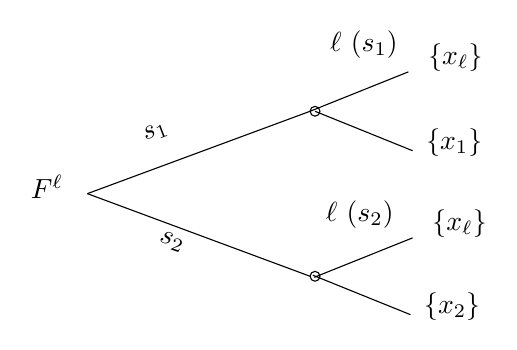
\begin{tikzpicture}[x=0.75pt,y=0.75pt,yscale=-1,xscale=1]
			%uncomment if require: \path (0,300); %set diagram left start at 0, and has height of 300

			%Straight Lines [id:da04967429201381823] 
			\draw [color={rgb, 255:red, 0; green, 0; blue, 0 }  ,draw opacity=1 ]   (246.33,115.1) -- (353.63,75.41) ;
			%Straight Lines [id:da4510990884707109] 
			\draw [color={rgb, 255:red, 0; green, 0; blue, 0 }  ,draw opacity=1 ]   (246.33,115.1) -- (353.63,154.91) ;
			%Shape: Circle [id:dp8318909509660006] 
			\draw  [fill={rgb, 255:red, 255; green, 255; blue, 255 }  ,fill opacity=1 ] (353.63,75.41) .. controls (353.63,74.09) and (354.69,73.03) .. (356,73.03) .. controls (357.31,73.03) and (358.38,74.09) .. (358.38,75.41) .. controls (358.38,76.72) and (357.31,77.78) .. (356,77.78) .. controls (354.69,77.78) and (353.63,76.72) .. (353.63,75.41) -- cycle ;
			%Shape: Circle [id:dp02055389565814525] 
			\draw   (353.63,154.91) .. controls (353.63,153.59) and (354.69,152.53) .. (356,152.53) .. controls (357.31,152.53) and (358.38,153.59) .. (358.38,154.91) .. controls (358.38,156.22) and (357.31,157.28) .. (356,157.28) .. controls (354.69,157.28) and (353.63,156.22) .. (353.63,154.91) -- cycle ;
			%Straight Lines [id:da6570820856056299] 
			\draw    (353.63,75.41) -- (401,56.41) ;
			%Straight Lines [id:da3482370480014345] 
			\draw    (355.63,155.41) -- (403,136.41) ;
			%Straight Lines [id:da8263111947331077] 
			\draw    (356,75.41) -- (403,94.41) ;
			%Straight Lines [id:da7257991174153424] 
			\draw    (355,154.41) -- (402,173.41) ;

			% Text Node
			\draw (270.54,83.19) node [anchor=north west][inner sep=0.75pt]  [color={rgb, 255:red, 0; green, 0; blue, 0 }  ,opacity=1 ,rotate=-339.07]  {$s_{1}$};
			% Text Node
			\draw (217.83,104.7) node [anchor=north west][inner sep=0.75pt]    {$F^{\ell }$};
			% Text Node
			\draw (281.77,131.06) node [anchor=north west][inner sep=0.75pt]  [color={rgb, 255:red, 0; green, 0; blue, 0 }  ,opacity=1 ,rotate=-19.16]  {$s_{2}$};
			% Text Node
			\draw (409.33,41.4) node [anchor=north west][inner sep=0.75pt]  [color={rgb, 255:red, 0; green, 0; blue, 0 }  ,opacity=1 ]  {$\{x_{\ell }\}$};
			% Text Node
			\draw (411.33,121.4) node [anchor=north west][inner sep=0.75pt]  [color={rgb, 255:red, 0; green, 0; blue, 0 }  ,opacity=1 ]  {$\{x_{\ell }\}$};
			% Text Node
			\draw (408.33,82.4) node [anchor=north west][inner sep=0.75pt]  [color={rgb, 255:red, 0; green, 0; blue, 0 }  ,opacity=1 ]  {$\{x_{1}\}$};
			% Text Node
			\draw (407.33,161.4) node [anchor=north west][inner sep=0.75pt]  [color={rgb, 255:red, 0; green, 0; blue, 0 }  ,opacity=1 ]  {$\{x_{2}\}$};
			% Text Node
			\draw (362,35.4) node [anchor=north west][inner sep=0.75pt]    {$\ell \ ( s_{1})$};
			% Text Node
			\draw (360,117.4) node [anchor=north west][inner sep=0.75pt]    {$\ell \ ( s_{2})$};


		\end{tikzpicture}
	\end{center}

	For each \( S \) define distorted likelihoods:

	\vfill

	\[
		\ell^{*}_S \in \left\{ \ell \in \Delta \left( S \right) \: \middle\vert \: F^{\ell} \succsim F^{\ell^{\prime}} \: \text{for all} \: \ell^{\prime} \in \Delta \left( S \right) \right\} .
	\]

	\begin{flushright}
		\hyperlink{distortedlikelihood}{\beamerbutton{Back}}
	\end{flushright}


\end{frame}

\end{document}